\documentclass[a4paper,12pt]{report}
% pacote da Língua Portuguesa%
\usepackage[utf8x]{inputenc}
\usepackage{indentfirst}
\usepackage{ucs}
\usepackage[brazil]{babel}
\usepackage[T1]{fontenc}

%pacotes matemáticos e separação entre linhas%
\usepackage{units, amstext, amsmath, stfloats, amssymb, graphics, setspace,dcolumn}
\usepackage{gensymb}
\usepackage{pdflscape}
\usepackage{booktabs} 
\usepackage{enumerate}
\usepackage[pdftex]{graphicx}
\usepackage{subfigure}
\usepackage{geometry}
\geometry{hmargin={2.5cm,2.5cm},vmargin={1.5cm,2cm}}
\usepackage{natbib}
\usepackage[pdftex]{hyperref} %Inserindo Links
\usepackage{pdfpages} %Inserindo PDFs
\makeindex
\usepackage[nottoc]{tocbibind}

\begin{document}
\setcounter{page}{1} \pagenumbering{Alph}

% Add PDF bookmark 
\pdfbookmark[0]{Title}{Title}

\thispagestyle{empty}
\begin{flushleft} ~\\ \vspace{-10mm} \hspace{-5mm}  
\includegraphics[width=40mm, height=10mm]{mcti} 
\begin{flushright}~\\ \vspace{-20mm} \hspace{-9mm}  
\includegraphics[width=30mm, height=10mm]{dppg} 
\end{flushright}


~\\ \begin{center} 
\includegraphics[height=50mm]{logo_on}  \end{center} % gráficos
~\\ \vspace{5mm}
\begin{centering}
\LARGE \textbf{Análise da Estrutura da Crosta na Região da Faixa Ribeira (entre as Províncias do Cráton São Francisco e da Bacia do Paraná) usando Métodos Sismológicos}
\\ \vspace{20mm}
\Large \textbf{Diogo Luiz de Oliveira Coelho} \\
\vspace{20mm}
\Large Dissertação para obter o grau de Mestre em
\\ \vspace{2mm}
\LARGE \textbf{Geofísica}
\\ \vspace{20mm}

\Large Orientador\\
\textbf{Stéphane Gerard Martial Drouet} \\
\Large Coorientador\\
\textbf{Bruno Yann Nicolas Goutorbe} \\
 
\vspace{20mm}

Rio de Janeiro \\
2015 \\
\end{centering}
\let\thepage\relax
\end{flushleft}
\pagebreak
\begin{titlepage}
 \vfill
  \begin{center}

   {\Large \textbf{Análise da Estrutura da Crosta na Região da Faixa Ribeira (entre as Províncias do Cráton São Francisco e da Bacia do Paraná) usando Métodos Sismológicos}} \\[2.5cm]

   {\large \textbf{Diogo Luiz de Oliveira Coelho}}\\[4cm]

   \hspace{.45\textwidth} %posiciona a minipage
   \begin{minipage}{.5\textwidth}
   \large Dissertação apresentada ao corpo docente do Programa de Pós-graduação em Geofísica do Observatório Nacional como parte dos requisitos necessários para a obtenção do grau de Mestre em Geofísica.\\[1cm]
  \end{minipage}

\begin{tabular}{c}
\hline
Orientador - Stéphane Gerard Martial Drouet \\ 
\bigskip\\
\hline
Banca - Ser Humano 1 \\ 
\bigskip\\
\hline
Banca - Ser Humano 2 \\ 
\bigskip\\
\hline
(Suplente) - Ser Humano 3 \\ 
\bigskip\\
\hline
(Suplente) - Ser Humano 4 \\ 
\bigskip\\
\end{tabular}
  \vfill

\vspace{2cm}

RIO DE JANEIRO \\
2015 \\

\end{center}
\end{titlepage} 
\pagenumbering{Roman}
\chapter*{Dedicatória}

\null\vskip15cm%
\begin{flushright}
    a quem não acredita na existência de sanduíche natural...
\end{flushright}
\vfill\newpage

\cleardoublepage
\chapter*{Agradecimentos}	
\chapter*{Epígrafe}

\null\vskip15cm%
\begin{flushright}
    \textit{There may be many earths, but there's only one Earthshaker.}
    \hspace{10cm}\textit{Raigor Stonehoof}  
\end{flushright}
\vfill\newpage

\cleardoublepage
\chapter*{Resumo}	
\chapter*{Abstract}
\addcontentsline{toc}{chapter}{Abstract}
\listoffigures
\listoftables
\tableofcontents

\pagenumbering{arabic}
\chapter{Introdução}

A integração de dados geológicos e geofísicos multidisciplinares é a maneira de se conseguir galgar degraus no entendimento e na compreensão do arcabouço geológico complexo de nosso país. Para tal o Observatório Nacional juntamente com a Petrobras começaram uma parceria, e executaram o projeto “Imageamento Subsal pela Utilização Conjunta de Migração Pré-empilhamento em Profundidade, do Método Magnetotelúrico Marinho e do Método Gravimétrico” da Rede Temática de Estudos Geotectônicos da Petrobras. Esta integração de dados é vanguardista no Brasil, constituindo-se um modelo de estudos na exploração de hidrocarbonetos e também em estudos geotectônicos. O Observatório Nacional realizou levantamentos geofísicos na porção sudeste brasileira, especificamenteo entre a Faixa Brasília e a Faixa Ribeira. 

Esta dissertação apresentará os dados coletados de estações sismográficas instaladas neste projeto e os resultados gerados serão integrados com resultados de outros métodos geofísicos, e estes servirão como subsídios para uma melhor interpretação geológica da região. 

A área de estudo encontra-se sobre terrenos policíclicos referíveis ao sul do Cinturão de Dobramentos Ribeira, nomeada por \cite{Riccomini_1989}, Sul do Cráton São Francisco e Sul da Faixa Brasília \citep{Almeida_Carneiro_1998}. Nessa região há um retrabalhamento de ciclos orogênicos pretéritos e o conjunto litológico é recortado por um sistema de falhas transcorrentes (zonas de cisalhamento) orientados segundo a estruturação regional, direção ENE a EW  \citep{Hasui_Sadowski_1976}. As feições estruturais da região de estudo são fortemente influenciadas pela Faixa Ribeira, devido a isso existe uma zona de interferência com a Faixa Brasília e com o Cráton do São Francisco \citep{kuhn_metamorphic_2004}; \citep{heilbron_evolution_2010}; \citep{valeriano_u_pb_2011}; \citep{heilbron_serra_2013}.

A Faixa Ribeira já foi alvo de diversos estudos sismológicos para uma melhor entendimento das estruturas crustais. Autores como \cite{Bassini_1986}, \cite{souza_crustal_1991}, \cite{souza_shear-wave_1995}, \cite{assumpcao_crustal_2002}, \cite{dias_cario_crustal_2006} e \cite{sand_franca_crustal_2004} já propuseram modelos de velocidade crustais para a região. Além disso existem inúmeros trabalhos geofísicos que também geraram conhecimento sobre a estruturas em subsuperfície, como os trabalho de \cite{flora_solon_ancient_2013}, \cite{Silva_2014}. 

Neste trabalho, para a análise da estrutura crustal da região utilizou-se de dois métodos sismológicos que se baseiam-se num princípio simples: a determinação das velocidades de propagação das ondas sísmicas e a procura de um modelo que melhor se ajuste às velocidades encontradas. A resolução dos modelos obtidos depende do tipo de onda utilizado e da geometria espacial das estações sismográficas segundo à fonte do sinal. Para isso fez-se uso de dois métodos complementares, um para obter informações de regiões profundas da crosta, Função do Receptor, o outro foi utilizado para extrair informações mais rasas sobre a estrutura crustal, Correlação de Ruído Ambiental.

Para o cálculo a espessura crustal na região utilizou-se o método da Função do Receptor, que foi desenvolvido por \cite{clayton_source_1976}, \cite{Langston_1977}, \cite{ammon_isolation_1991}, \cite{cassidy_numerical_1992}, \cite{Zhu_Kanamori_2000}. Tal método faz uso do sinal de tele-sismos para inferir a profundidade da discontinuidade de Mohorovicic. Já para extrair informações sobre as estruturas crustais rasas utilizou-se as correlações cruzadas do ruído sísmico ambiental entre pares de estações para medir a dispersão das ondas Rayleigh nas camadas mais superficiais, inicialmente prosposto por \cite{aki_space_1957}, porém, somente \cite{campillo_long-range_2003}  e \cite{shapiro_emergence_2004} mostraram, pela primeira vez, a  presença de ondas superficiais nas correlações cruzadas de ruído sísmico.

O objetivo deste trabalho é a análise e delimitação de grandes feições estruturais crustais através de perfis de Funções do Receptor da onda P e de mapas tomográficos de velocidade gerados a partir das estações temporárias do projeto SUBSAL mais algumas estações da Rede Sismográfica Brasileira (RSBR, \url{www.rsbr.gov.br}).
\chapter{Contexto Geológico}
\date{24}{03}{2015}


A área de estudo enquadra-se geolologicamente no Rift Continental do Sudeste do Brasil(RCSB) sobre terrenos policíclicos referíveis ao sul do Cinturão de Dobramentos Ribeira, nomeada por \cite{Riccomini_1989} em seu trabalho, Sul do Cráton São Francisco e Sul da Faixa Brasília, como pode ser observado na Figura \ref{mapa_geologico}. Essa zona geológica é intulada por \cite{Almeida_Carneiro_1998} como Planalto Atlântico. Encontra-se nessa região retrabalhamento de ciclos orogênicos pretéritos e o conjunto lito1ógico é recortado por um sistema de falhas transcorrentes (zonas de cisalhamento) orientados segundo a estruturação regional, direção ENE a EW, \cite{Hasui_Sadowski_1976}. As feições estruturais da região de estudo são fortemente influenciadas pelo Cinturão de Dobramentos Ribeira.

As bacias sedimentares presentes na área de estudo estão alojadas na região do Rift Continental do Sudeste do Brasil (RCSB), como pode ser visto na Figura \ref{mapa_estacoes_geologico}. \cite{Riccomini_1989} apresenta o RCSB como uma depressão alongada e deprimida com mais de 900 km de comprimento entre os estados Paraná e Rio de Janeiro. Este Rift possui uma idade paleógena e segue a linha de costa atual, alcançando o Oceano Atlântico em seu segmento ocidental e na sua Terminação nordeste. Inúmeros corpos alcalinos de idade cretácica a paleogênica ocorrem ao longo das bordas desse sistema de Rifts. A área em estudo engloba o segmento central do RCSB. Este possui as bacias sedimentares de São Paulo, Taubaté, Resende e Volta Redonda, como pode-se observar nas áreas com tonalidades em amarelo na Figura \ref{mapa_estacoes_geologico}. 

É visível a presença de corpos arredondas nas Figuras \ref{mapa_geologico} e \ref{mapa_estacoes_geologico}, tais corpos representam plútons alcalinos cretácicos e cenozóicos. \cite{MOTA_2012} mostra que as intrusões alcalinas geram grandes desníveis topográficos, áreas elevadas que podem atingir 800 metros acima do nível do mar. Essas rochas estão alinhadas na direção WSW-ENE, como pode ser visto na Figura \ref{mapa_geologico}. A maior parte desses corpos magmáticos é formada por sienitos e monzonitos, com variações texturais desde plutônicas a subvulcânicas.

\begin{figure}[!ht]
\centering
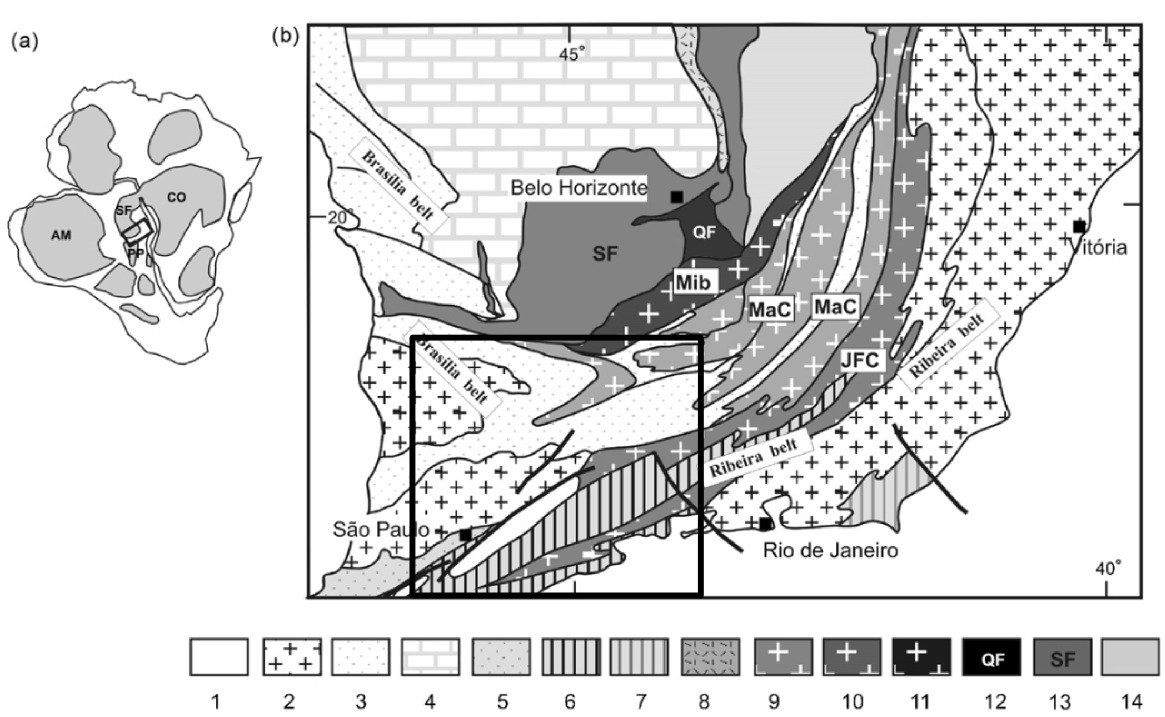
\includegraphics[scale=0.5]{Figs/mapa_geologico.png}
\caption[Mapa tectônico da Região do Sudeste do Brasil segundo  \cite{trouw_new_2013}.]{Mapa tectônico da Região do Sudeste do Brasil com a área de trabalho marcada pelo quadradro. Legenda: 1-Bacias do Paraná e do Rift Cenozóico. 2-Plutons alcalinos Cenozóicos/Cretácios. Cráton São Francisco e Bacias interiores (3–5), 3-Embasamento; 4-Cobertura (Grupo Bambuí); 5-Cobertura (rochas metasedimentares autóctones e paraautóctones. Orógeno Brasília (6-9) 6-Sistema de \textit{Nappe} Andrelândia(AND) e \textit{Nappe} Passos(P);7-\textit{Nappe} Socorro(S)-Guaxupé(G); 8- Terreno Embu(E)-Paraíba do Sul(PS); 9-Terreno Apiá. Orógeno Ribeira(6-14), 10-Domínio Externo; 11- Domínio Juiz de Fora; 12-Arco Rio Negro(Terreno Oriental); 13-Terreno Oriental; 14- Terreno Cabo Frio. A área demarcada com a linha tracejada cobrindo a parte sul da Faixa Brasília e a parte sudeste do Cráton São Francisco corresponde a uma zona de interferência onde a deformação e o metamorfismo da Faixa Ribeira se  sobressai na Faixa Brasília. Adaptado de \cite{trouw_new_2013}}
\label{mapa_geologico}
\end{figure} 

O sul da Faixa Brasilía foi descrito, \cite{pimentel_tectonic_2011},\cite{reno_situ_2012} e \cite{trouw_new_2013}, como resultado da colisão entre a margem passiva do paleocontinente São Francisco do leste com a margem ativa do bloco, ou paleocontinente, Paranapanema do lado oeste da sutura, observado no perfil A-B na Figura \ref{perfil_esquematico}. Esta colisão produziu um empilhamento espesso de \textit{nappes} ao longo da sutura, como o Sistema de \textit{Nappe} Andrelândia(ANS), que pode ser observado nos perfis mostrados no perfil A-B mostrado na Figura \ref{perfil_esquematico}. Dobras em bainha em grande escala e inúmeras dobras interropidas atestam a deformação dúctil intensa dentro das \textit{Nappes}. Lineamentos alongado, combinados com indicadores de cisalhamento mostram do norte para o sul a troca progressiva, cavalgando do topo para E-SE  na \textit{Nappe} Passos. A sutura desse cinturão é interpretada sendo localizada entre a \textit{Nappe} Socorro-Guaxupé e o Sistema \textit{Nappe} Andrelândia, como mostrado no perfil C-D na Figura \ref{perfil_esquematico}.

\begin{figure}[!ht]
\centering
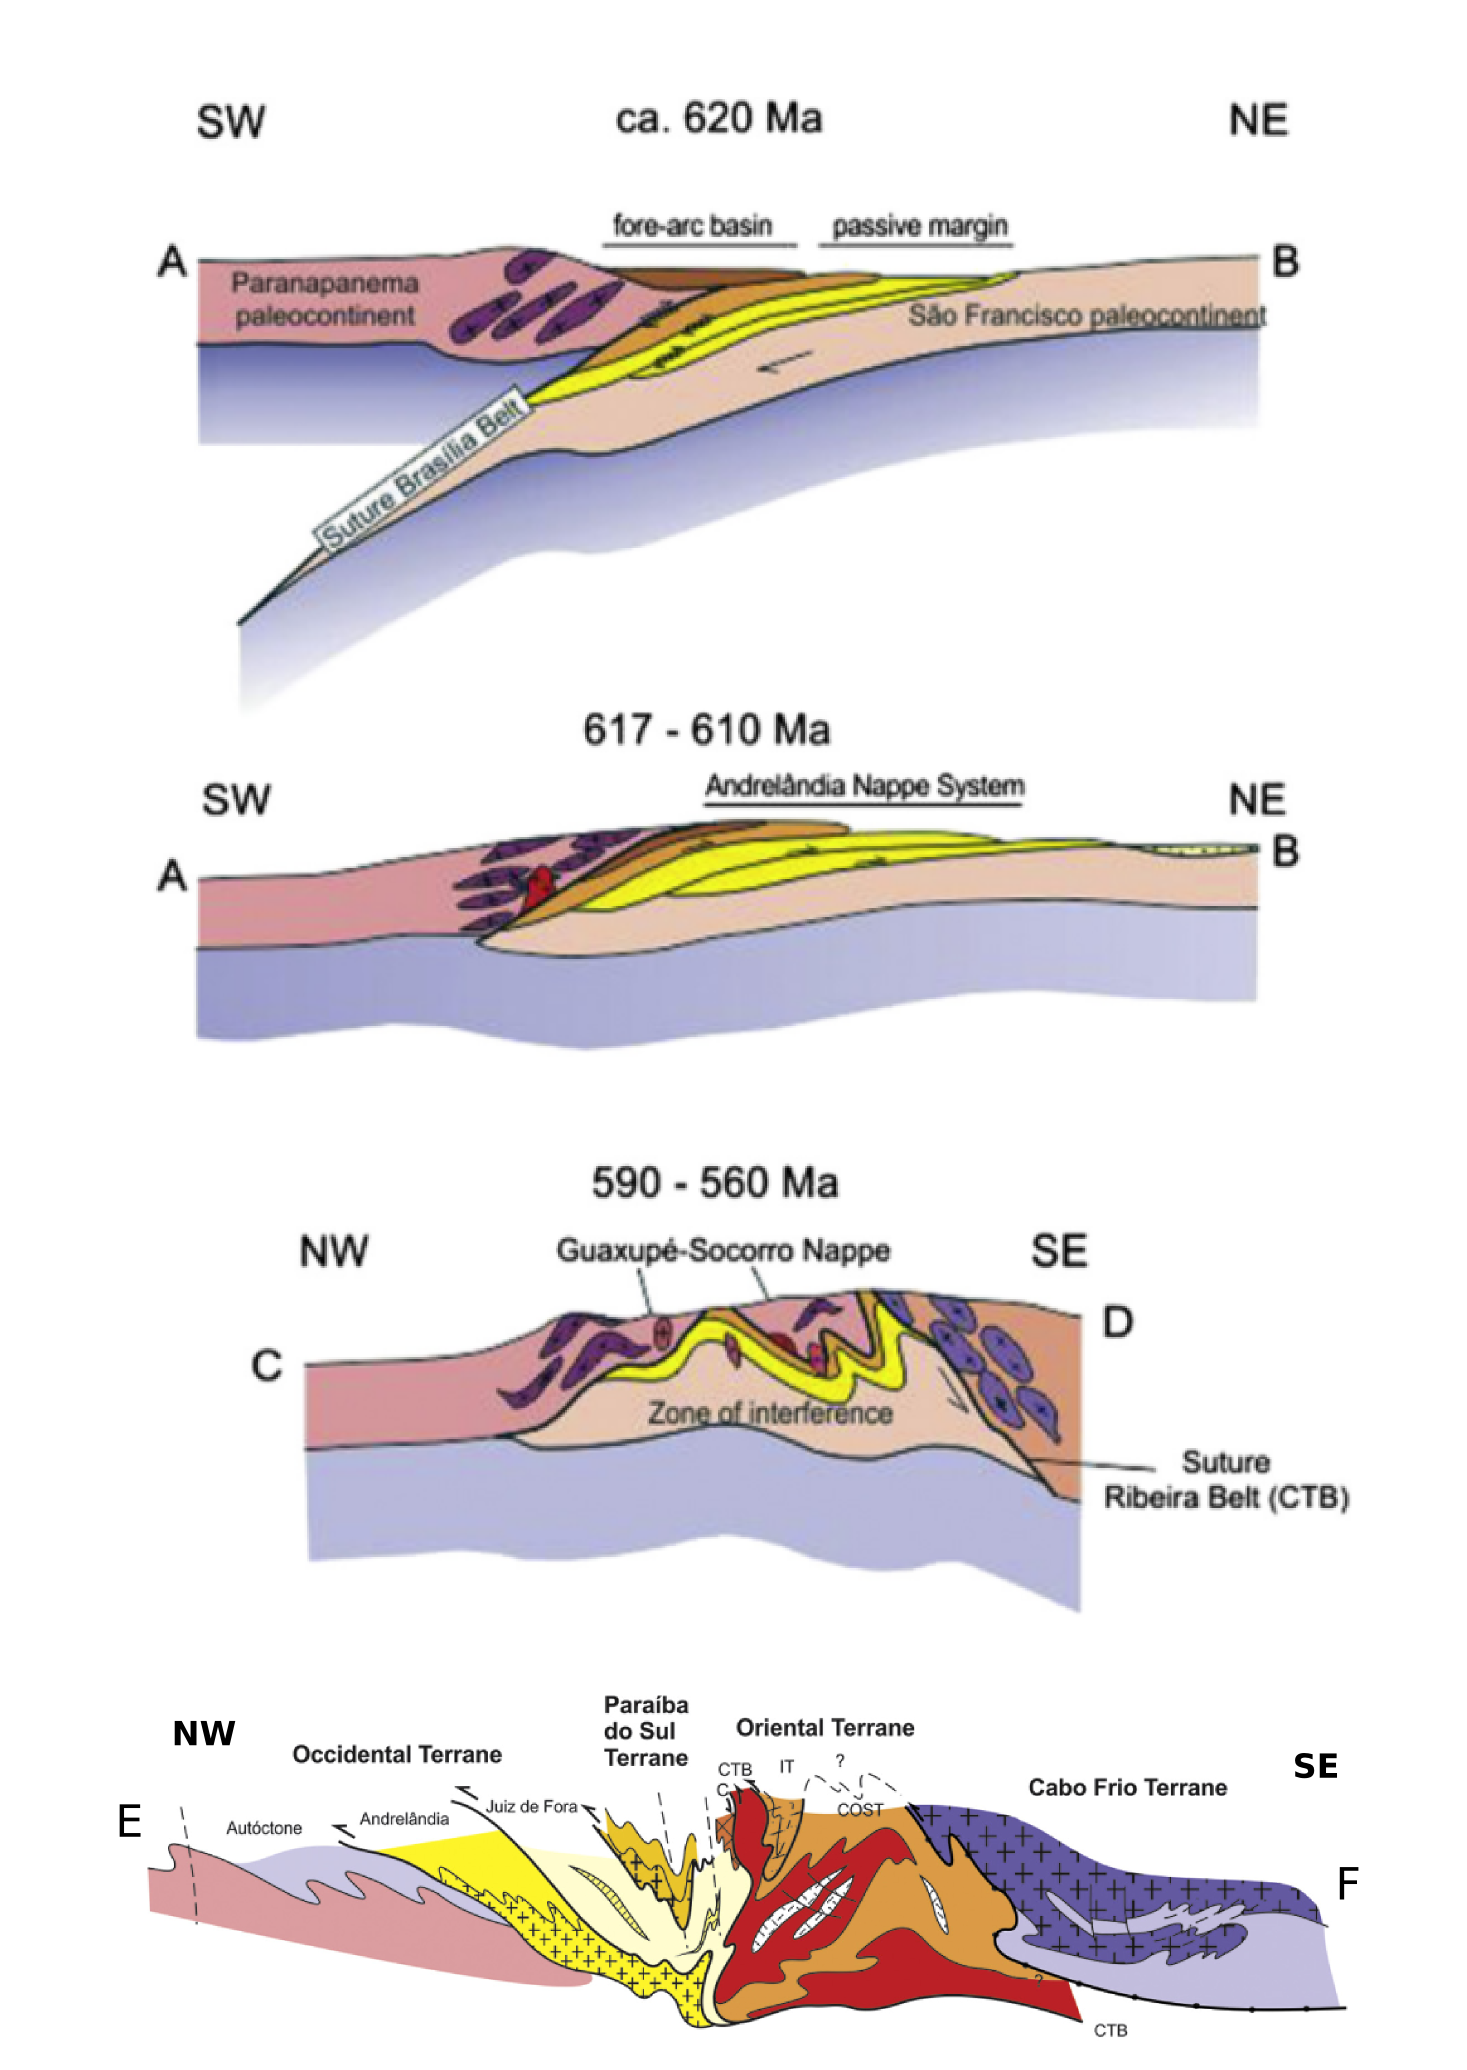
\includegraphics[scale=0.5]{Figs/perfil_esquematico_area.png}
\caption[Perfis Esquemáticos da Região do Sudeste do Brasil segundo  \cite{trouw_new_2013}.]{Perfis Esquemáticos marcados na Figura \ref{mapa_geologico} mostrando a evolução da superposição na zona de interferência. Retirado de \cite{trouw_new_2013}}
\label{perfil_esquematico}
\end{figure} 

A Faixa Ribeira é composta por rochas metamórficas, migmatitos e granitóides relacionados ao Ciclo Orogenético Brasiliano, como citam \cite{kuhn_metamorphic_2004}, \cite{heilbron_evolution_2010} e \cite{valeriano_u_pb_2011}. Esta tendência estrutural regional NE-SW pode ser observada na Figura \ref{mapa_geologico}. Segundo \cite{heilbron_evolution_2010} a Faixa Ribeira é composta por 4 terrenos tectônicos-estratigráficos separados por falhas de
empurrão ou por zonas de cisalhamento oblíquas transpressivas: (a) a margem retrabalhada do Cráton São Francisco definida como Terreno Ocidental; (b) O Terreno Paraíba do Sul-Embú que está cavalgando sobre o Terreno Ocidental;(c) O Terreno Oriental (Serra do Mar) que inclui o Arco Magmático Neoproterozóico, e (d) O Terreno Cabo Frio, que foi acrescionado depois, por volta de 520 M.a. Estes Terrenos estão demarcados na Figura \ref{mapa_geologico}. Estes são subdivididos em vários domínios, tais domínios são identificados devido ao seu contraste litológico, geoquímica isotópica e geocronologia, cita \cite{kuhn_metamorphic_2004}. A sutura entre o Terreno Ocidental e Oriental é uma zona de cisalhamento mergulhando para noroeste (NW), também chamada de Limite Tectônico Central, \textit{Central Tectonic Boundary}(CTB) por \cite{heilbron_evolution_2010} e \cite{trouw_new_2013}, demarcada na Figura \ref{mapa_geologico}. Essa sutura pode ser mapeada continuamente por pelo menos 200 km entre a costa de São Paulo e a Serra do Órgãos, no estado do Rio de Janeiro. 

\cite{trouw_new_2013} sumariza as principais características dos terrenos que compõem a Faixa Ribera. O Terreno Ocidental é caraterizado por rochas do embasamento Paleoproterozóico a Arqueano, representado pelos Complexos Barbacena, Mantiqueira e Juiz de Fora, e por uma cobertura siliciclástica metamorfizada oriunda de uma margem passiva. Esta é chamada de Megassequência Deposicional Andrelândia. Já o Terreno ou Klippe Paraíba do Sul possui ortognaisses granodioríticos a graníticos do Complexo Quirino, de idade Paleoproterozóica e é coberta por rochas do Complexo Paraíba do Sul, gnaisses feldspáticos e pelíticos, com intercalações de mármores dolomíticos. O Terreno Oriental aloja ortognaisses tonalíticos a granodioríticos pertencentes ao Complexo Rio Negro, bem como metassedimentos Neoproterozóicos, ricos em intercalações carbonáticas e rochas metabásicas. A Colisão deste terrenos acarretou na geração de vários tipos de rochas granitóides sin-colisionais: leucogranitos, charnockitos, granitos porfiróides e bitotita granitos. Por fim, o Terreno Cabo Frio engloba ortognaisses Paleoproterozóicos do Complexo Quirino e uma sucessão metassedimentar com gnaisses pelíticos com cianita, sillimanita e granada, metabasitos e rochas calcissilicáticas. 

\begin{figure}[!ht]
\centering
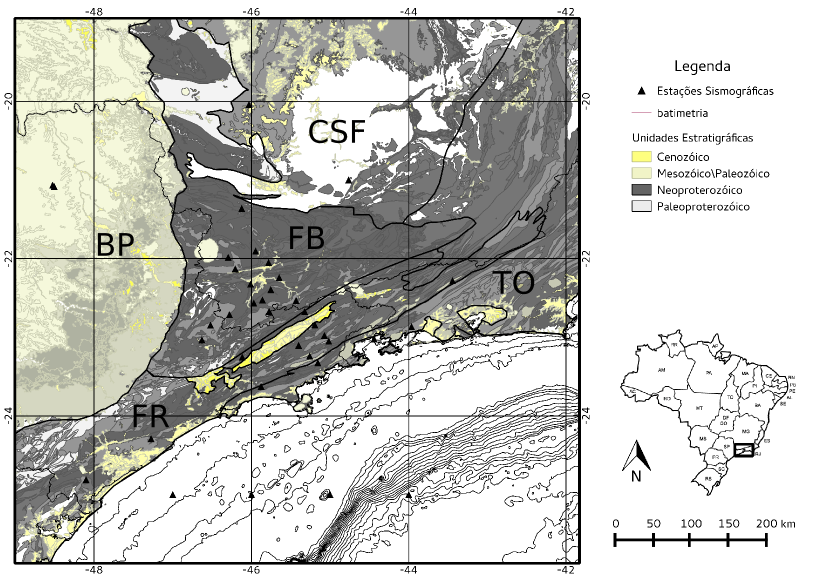
\includegraphics[scale=0.5]{Figs/mapa_estacoes_geologico.png}
\caption[Mapa de localização das Estações Sismográficas na região com o mapa geológico simplificado.]{Mapa de localização das Estações Sismográficas utilizadas neste trabalho e o mapa simplificado das unidades estratigráficas e tectônicas. BP-Bacia do Paraná, CSF-Cráton São Francisco, FB-Faixa Brasília, FR-Faixa Ribeira, TO-Terreno Oriental.}
\label{mapa_estacoes_geologico}
\end{figure}


\chapter{Aquisição e Tratamento dos Dados}	
\today
\section{Aquisição de Dados}

No âmbito do projeto SUBSAL, realizado conjuntamente entre o Observatório Nacional e a Petrobras,  instalou-se 24 estações sismográficas temporárias banda larga (STS2 ou Reftek RT151-120s), as coordenadas de cada estação pode ser vista na Tabela \ref{tabelaDATA}. Cuja a faixa de frequência registrada varia de 50 Hz até 100 segundos. Acoplado a este sistema temos um conjunto de baterias, reguladores, painel solar e o registrador, onde são armazenados os dados. O sistema armazena os dados em um disco de 4Gb que é retirado em cada campanha de coleta dos dados.

Mesmo se tratando de estações temporárias, as instalações devem conter os requisitos mínimos para a uma aquisição confiável dos dados. Principalmente assegurar que o sensor e o registrador não sofram com as intempéries climáticas ou com danos causados pela passagem de animais ou pessoas pelo local. A Figura \ref{instalacao} mostra como é o fluxo de trabalho dos funcionários do Observatório Nacional no campo para a instalação das estações sismográficas temporárias. 

A Figura \ref{instalacao}-A mostra que o sensor deve ser acoplado à rocha sã. Com a ajuda de uma bússola o sensor é orientado segundo um azimute.  Porém para um isolamento térmico, crucial para o bom funcionamento do sismômetro, pinta-se a área com um tinta isolante e o sismômetro é revestido com uma manta térmica, como pode ser visto na A Figura \ref{instalacao}-B e \ref{instalacao}-C. Logo após instala-se as baterias e o sensor é mais uma vez revestido. Para a absorçao da umidade de todo o sistema da estaçao, utiliza-se carvão e sílica em gel, como pode ser visto na Figura \ref{instalacao}-D. Em seguida todo o sistema é coberto por uma nova estrutura para evitar as intempéries e cercada para isolar a área, como pode ser visto nas Figuras \ref{instalacao}-E e F.	  

\begin{figure}[!ht]
\centering
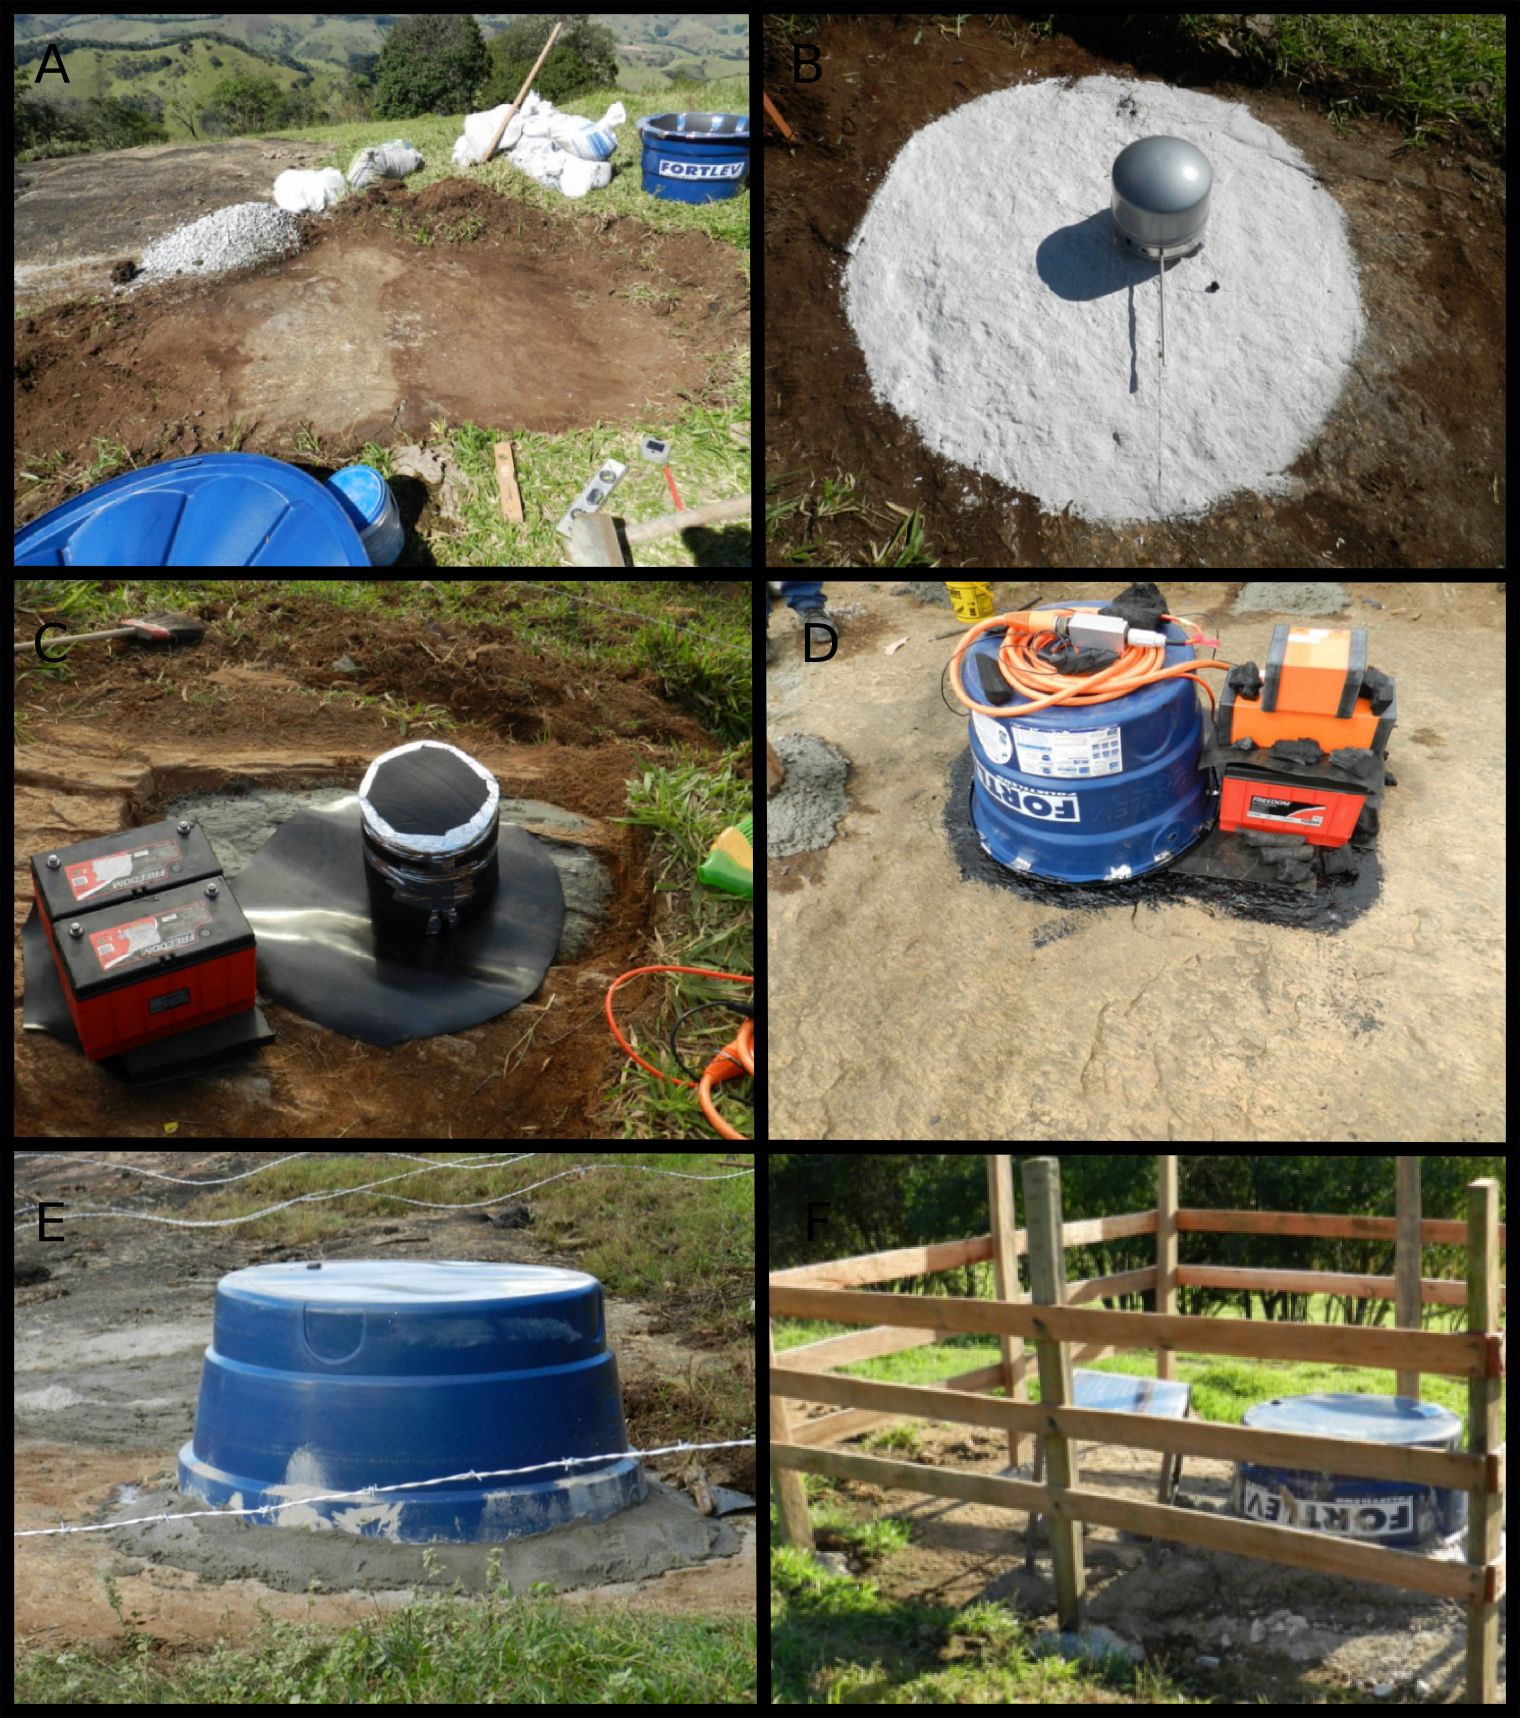
\includegraphics[scale=0.5]{Figs/instalacao.png}
\caption[Mosaico mostrando como é feita a instalação das estações sismográficas temporárias do projeto SUBSAL.]{Mosaico mostrando como é feita a instalação das estações sismográficas temporárias do projeto SUBSAL. As figuras mostram os diferentes estágios na instalação das estações.}
\label{instalacao}
\end{figure} 

As estações foram dispostas espacialmente em três perfis em relação à costa, dois perpendiculares à costa, perfil 1 a oeste e perfil 2 a leste, e um paralelo, perfil 3, como observado na Figura \ref{map_loc}. O perfil 1 estende-se da estação STA01, localizada próximo à costa, até a STA09. O perfil 2 vai da estação STA10, ao norte, até a STA16, próximo à costa. O perfil 3 é da estação STA17, oeste, até a STA24, leste. A distância entre as estações é aproximativamente de 20 km. As coordenadas das estações são dadas na Tabela \ref{tabelaDATA}. 

\begin{figure}[!ht]
\centering
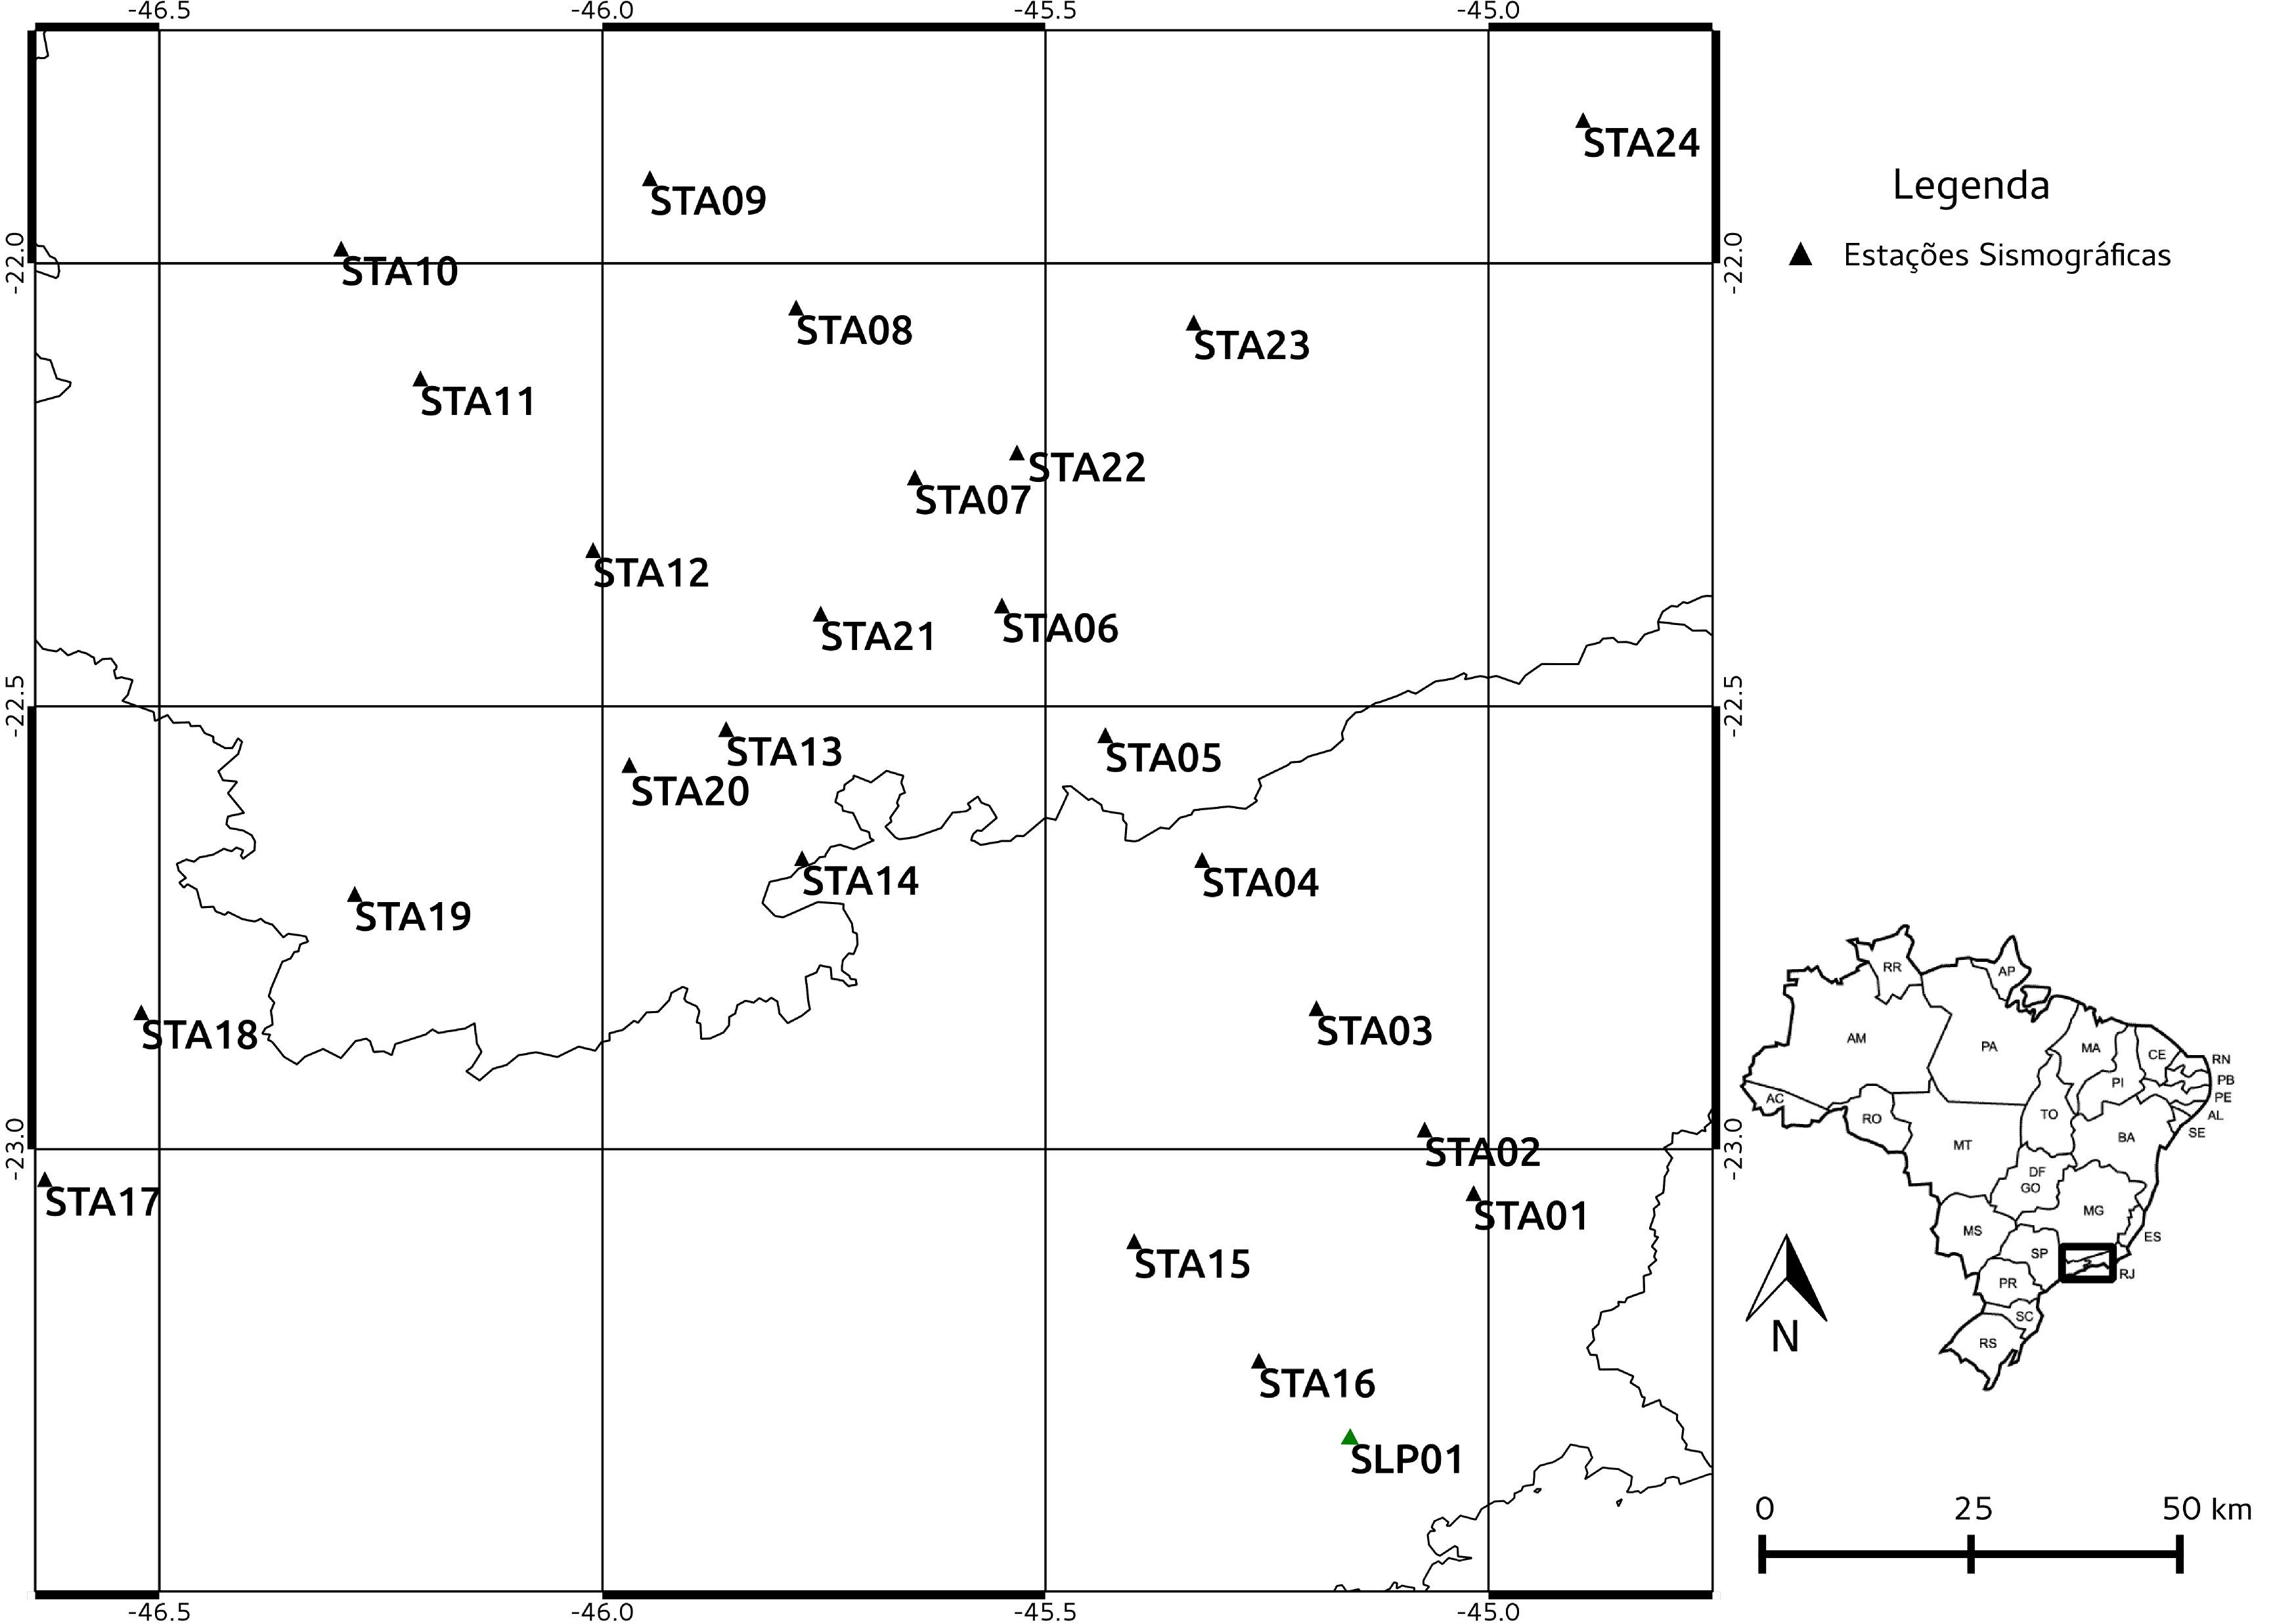
\includegraphics[scale=0.4]{Figs/mapa_das_estacoes_simosgraficas_instaladas.png}
\caption{Mapa das estações sismográficas instaladas (triângulos vermelhos). Os outros triângulos são estações da Rede Sismográfica Brasileira.}
\label{map_loc}
\end{figure}

O período de operação das estações foi distinto para os perfis. Os dois perfis perpendiculares à costa foram instalados no meio do ano de 2012 e o perfil paralelo no final de 2012. As estações ficaram em fucionamento até o final do ano de 2013 registrando o movimento do terreno, as datas em que as estações ficaram em funcionamento podem ser encontradas na Tabela \ref{tabelaDATA}. 

A velocidade do meio é registrada pelo sismógrafo, através de sensores verticais e horizontais em três componentes. Pode ser visto na Figura \ref{simograma} o deslocamento do meio que é encontrado através da integração dos registros de velocidade. Esse registro da variação da amplitude resultante em uma série temporal é chamado de sismograma. 

\begin{figure}[!ht]
\centering
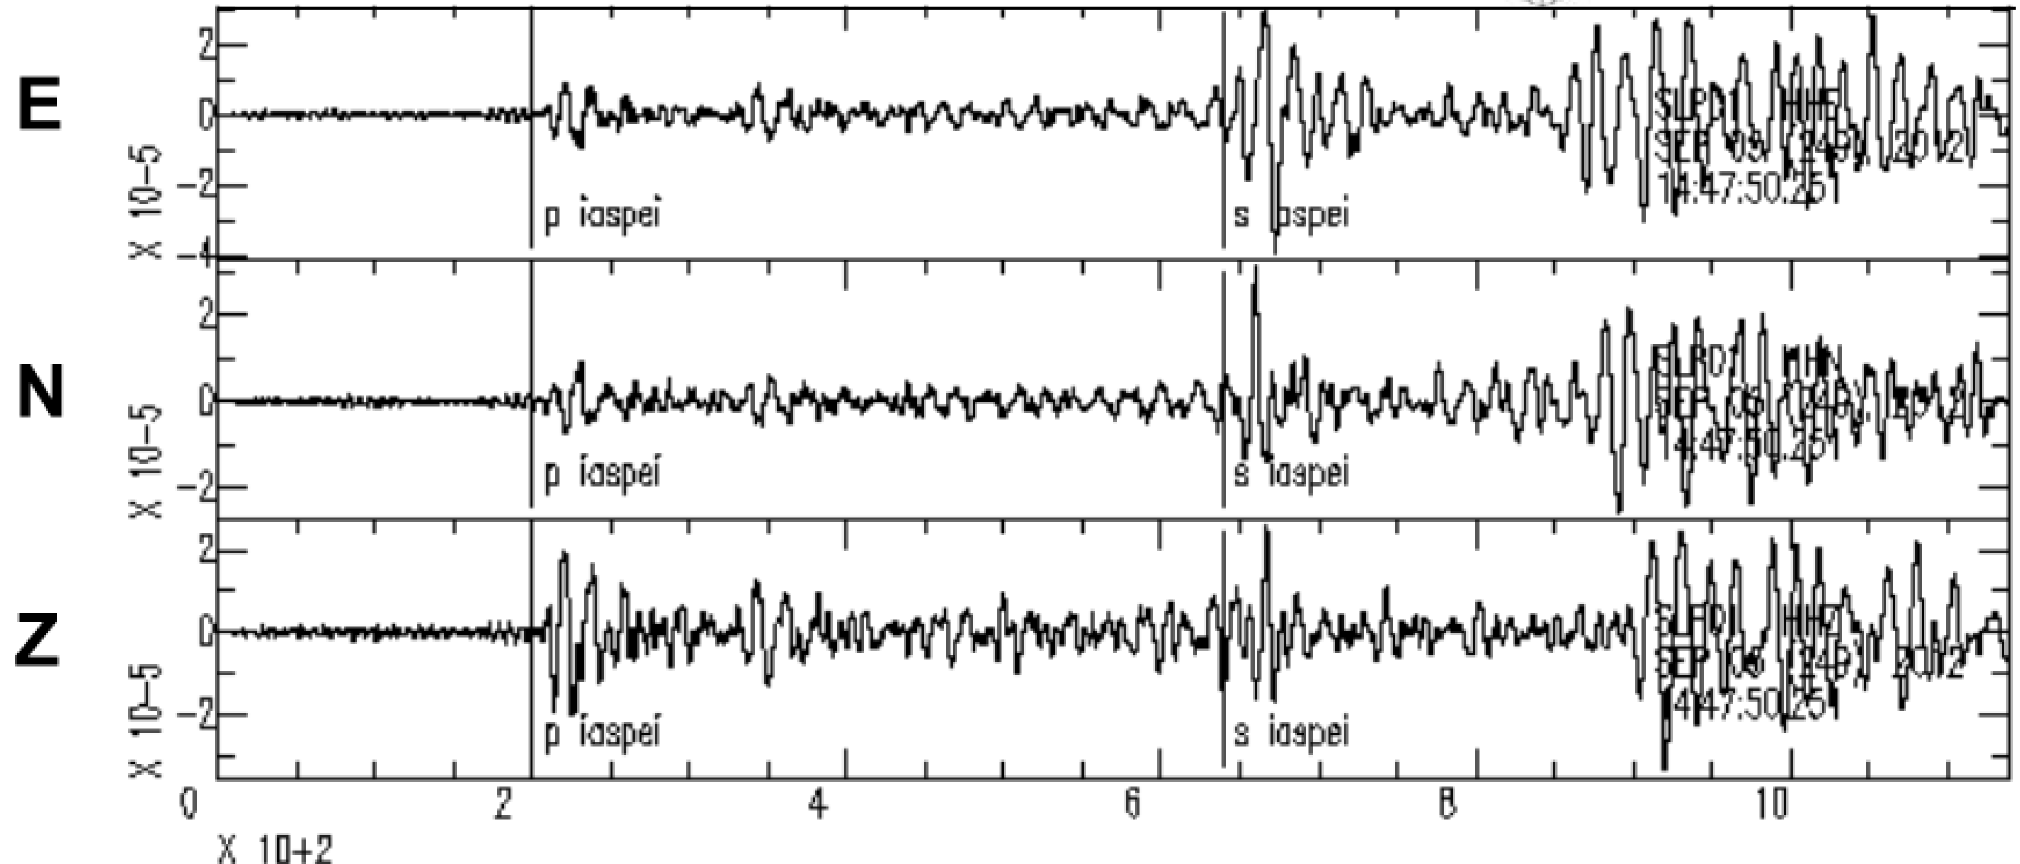
\includegraphics[scale=0.6]{Figs/sismograma.png}
\caption{Sismograma mostrandos as três componentes do deslocamento do terreno.}
\label{simograma}
\end{figure}

O sismograma é gerado pela perturbação do meio pelas ondas  mecânicas que se propagam no interior da Terra. Essas ondas tem velocidades variando em função dos parâmetros elásticos do meio e da densidade. E estes variam pela mineralogia e condições de pressão e temperatura do meio atravessado. As ondas mecânicas são divididas em ondas de corpo e de superfície. As ondas de corpo estão categorizadas em dois tipos: as ondas P, longitudinal, e as ondas S, transversais. A onda P é mais rapida e que consegue se propagar em todos os meios, tem velocidade entre 4 e 7 km$/$s na crosta terrestre e em torno de 8 km$/$s no manto superior. As ondas S tem velocidade menor do que a onda P, em torno de 3 a 4 km$/$s na crosta. porém a onda S não se propaga em meios líquidos.

Para produzir esta análise sobre a estrutura da região de estudo pelo Função do Receptor utilizou-se de um conjunto de dados com eventos sísmicos registrados. O número de eventos utilizados no processamento varia devido ao nível de sinal-ruído da forma da onda, pois há uma necessidade de visualização clara da chegada da onda P, como pode ser constatado na Figura \ref{simograma}. Já para a Dispersão de Ondas de Superfície utilizou-se o ruído sísmico ambiental.

\section{Tratamento dos Dados}

A caracterização prévia das informações contidas no sinal é imprescindível para o processamento. A primeira avaliação da performance e da qualidade dos dados da estações sismográficas foram feitas no software livre PQLX.  A metodologia do PQLX é baseada no trabalho de \cite{McNamara_Buland_2004}. Esse procedimento é bastante usado para se obter a informação espectral sísmica.

No programa PQLX a série temporal é segmentada em intervalos de uma hora, com 50\% de superposição do sinal. Cada janela de hora está separada em 13 intervalos com 75\% de superposição para calcular a densidade de pontência espectral, \textit{Power Spectral Density}. As médias obtidas para cada um dos 13 intervalos são usadas para estimar as funções densidade de probabilidade, \textit{Probability Density Functions}, calculados a partir das médias pelo número total de segmentos de hora em hora. 

Essa metodologia de \cite{McNamara_Buland_2004} difere dos métodos habitualmente utilizados, porque não é necessário a visualização de todo conjunto de dados para uma estima qualitativa do sinal. É marcado na Figura \ref{PQLX} as curvas HNM e LNM, que são o maior nível de ruído  e o menor nível de ruído, respectivamente. Estes são valores padrões de diferentes estações, são utilizados para demarcar o limite mínimo e máximo que o nível de ruído pode chegar, mostrado por \cite{McNamara_Buland_2004}. A funções densidade de probalibilidade na Figura \ref{PQLX} mostram a distribuição das fontes de ruído sísmico. Frequências altas são dominadas por ondas de volume e períodos longos por ondas de superfícies. Como por exemplo, ruído cultural de alta frequência. Ruídos gerados por vento, água e pelo contexto geológico local se apresentam em períodos mais longons. Microssismos apresentam dois picos bem marcantes no espectro do ruído sísmico ambiental, um de 10-16 segundos conhecido como "pico de frequência único. Em altas amplitudes, picos de longo período, de 4-8 encontram-se os "picos de frequênacia duplas".  

\begin{figure}[!ht]
\centering
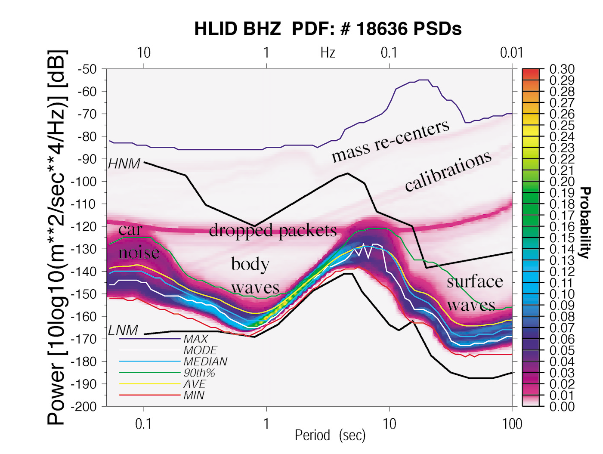
\includegraphics[scale=0.6]{Figs/mcnamura_buland.png}
\caption{Análise qualitativa do sinal atraves das \textit{Power Density Functions}. \cite{McNamara_Buland_2004} }
\label{PQLX}
\end{figure}

O produto de uma análise qualitativa premilinar nos gráficos gerados pelo programa PQLX é mostrado na Figura \ref{PQLX_results}, que tem como exemplos a componente HHZ nas estações STA05, STA04 e STA24. Observando os resultados nas estações temporárias conclui-se que existem registros bons e confiáveis, como exemplo a Figura \ref{PQLX_results}-A. Porém em algumas estações existem pequenos problemas, que são caracterizados por tendências lineares, como observados na Figura \ref{PQLX_results}-B. Já em outras estações pode-se constatar neste estudo preliminar a falta de registros na componente HHZ, que possivelmente é um problema no instrumento registrador ou no sensor, isto pode ser observado na Figura \ref{PQLX_results}-C.

\begin{figure}[!ht]
\centering
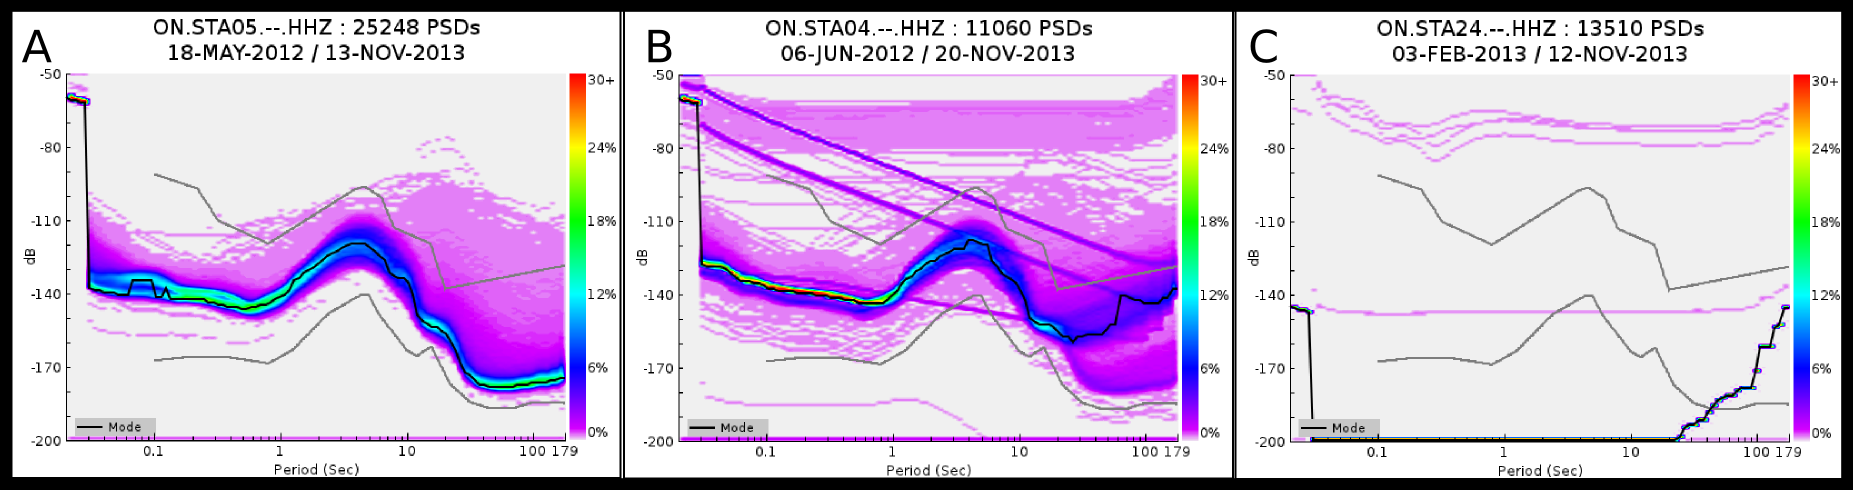
\includegraphics[scale=0.35]{Figs/pqlx_results.png}
\caption{Exemplos de resultados gerados pela análise qualitativa do sinal atraves do programa PQLX, que utiliza o método de \cite{McNamara_Buland_2004}.}
\label{PQLX_results}
\end{figure}

\subsection{Processamento para as Função do Receptor}

Os dados utilizados para os cálculos utilizando o método da Função do Receptor foram dados coletados das 24 estações temporárias da Rede SUBSAL e a estação permanente SLP01, esta pertecente a rede RSIS, parte da Rede Simosgráfica Brasileira (RSB), \url{www.rsbr.gov.br}, como pode ser visto na Figura \ref{map_loc}. Porém ao final agregou-se valores da profundidade de Moho de estações pertencentes à Universidade de São Paulo (USP), citados por \cite{Assumpcao_Brazil_2013}. 

Para assegurar a confiabilidade do processamento é necessário um tratamento preliminar dos sinais brutos. Utilizou-se eventos catalogados na rede IRIS para uma identificação automática nestes sinais. Alguns pré-requisitos foram utilizados para a escolha dos eventos, como:

\begin{enumerate}
\item Distância Epicentral;
\item Magnitude;
\end{enumerate}

Sismos próximos, com distância menor que 20 graus da estação estudada, geram ondas com incidência oblíqua e produzem uma triplicação característica. Esta se refere a fases de ondas sísmicas que possuem um parâmetro do raio similar e possuem os tempos de chegada bem próximos, logo devem ser processados de maneira diferente. Em sismos com distâncias maiores que 95 graus as ondas P não chegam na estação devido a inversão de velocidade no limite manto-núcleo, diminuição da velocidade da onda P entre o manto e o núcleo, e não é observada a onda P direta. Por isso a distância epicentral é tida como ideal entre 20 e 95 graus, como é observado na Figura \ref{mapa_eventos}. Devido grande parte dos sismos serem oriundos da Cordilheira dos Andes,como é visto na Figura \ref{teste_tempo}, também utilizou-se dados com distâncias menores que 20 graus. A magnitude do sismo é importante para a propagação da onda, eventos com pequena magnitude não tem energia suficiente para gerar um sinal claro no sismograma.

\begin{figure}[!ht]
\centering
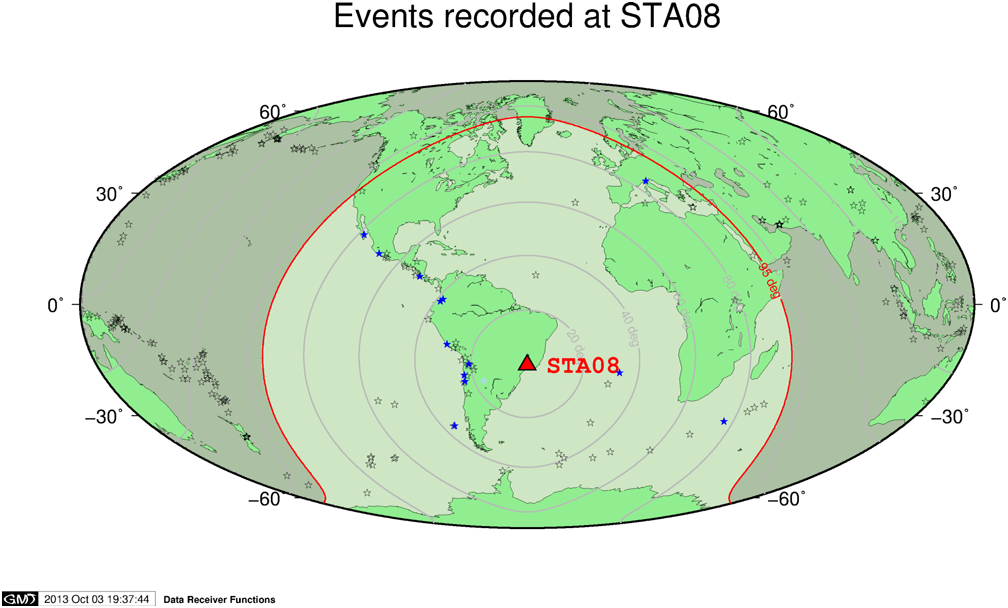
\includegraphics[scale=0.6]{Figs/mapa_de_eventos.png}
\caption[Mapa dos eventos registrados na estação STA08.]{Mapa dos eventos (estrelas) registrados na estação STA08. O limite de 95 graus está indicada em vermelho. Estrelas azuls mostram os eventos com dados de qualidade que são usadas no calculo das Funçoes do Receptor}
\label{mapa_eventos}
\end{figure}

Subsequentemente um foi feito um janelamento do registro 5 segundos antes e 10 segundos depois da chegada da onda P, esta é calculada pelo modelo de velocidade da Terra  IASPEI91 \citep{kennet_iaspei_1991}. Após a discriminação e o janelamento do sinal, examina-se visualmente cada registro para certificar que todos os eventos selecionados tem um nível de sinal-ruído bom e fazer a marcação do tempo de chegada da onda P, como na Figura \ref{simograma} . 

Logo após removeu-se a média e tendência linear dos dados. Aplicou-se um filtro passa-alta com freqüência de corte de 0.1 Hz para eventos com distância entre 20 e 95 graus e de 2 Hz para eventos próximos (<20). Os dados originais com amostragens a cada 0,01 segundos (100 Hz) são interpolados para gerar dados com amostragens cada 0,025 segundas (40 Hz), porque a informação de alta freqüência não é considerada nesta análise.

Após esta análise preliminar nos dados observou-se que algumas estações temporárias apresentaram problemas nos dados e tiveram que ser descartadas dessa análise. As estações STA23 e STA24 apresentaram a componente vertical com problemas, quebrada. Mas as outras componentes estão boas e poderam ser utilizadas em outros estudos. Já a estação STA22 só funcionou em poucos dias, como pode ser visto na Tabela \ref{tabelaDATA}.


\subsection{Dispersão de Ondas de Superfície}

Para o cálculo da dispersão das ondas de superfície utilizou-se estações temporárias da Rede SUBSAL, estações da Rede GEOSCOPE, pertencentes ao \textit{Institut de Physique du Globe de Paris} e do Projeto de Sísmica  da Litosfera Brasileira, pertencentes a Universidade de São Paulo (USP).

A garantia da fiabilidade do tempo de chegada da onda P é fundamental para o processamento gerar resultados consistentes. Pois ao contrário do método da Função do Receptor, que usa registros de uma mesma estação, o método da Dispersão de Ondas de Superfície utiliza dados de duas estações, logo tais estações devem estar sincronizadas. Portanto testes com o tempo de chegada da onda P forão feitos. \cite{gibbons_identification_2006} mostra que fazendo a correlação de dois eventos distantes em uma estação sismográfica consegue-se caracterizar esse tempo de chegada, como é visto na Figura \ref{teste_tempo}. \cite{gibbons_identification_2006} assume que  se não há alterações mensuráveis na velocidade da estrutura entre a fonte e os receptores, ondas sísmicas de dois eventos co-localizados terá a mesma duração de tempo para chegar a um determinado sensor. A função de correlação cruzada para um dado sinal a uma dada estação mede que a semelhança entre a porção posterior do sismograma é a do modelo de forma de onda. O tempo de separação entre o início do modelo e o valor máximo da função de correlação cruzada deve ser igual ao tempo que separa os dois tempos de origem dos eventos para todas as estações. Qualquer discrepância nos tempos de separação medido em duas estações diferentes, o que não é atribuível a diferença entre fontes ou uma SNR baixa, deve ser o resultado de uma anomalia em sincronismo um, ou ambos, dos instrumentos.

\begin{figure}[!ht]
\centering
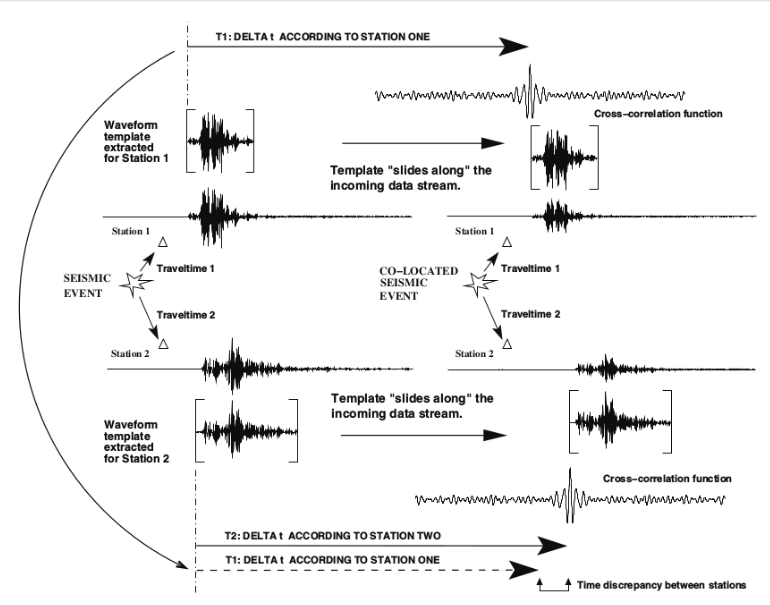
\includegraphics[scale=0.7]{Figs/correlacao_tempo_de_chegada.png}
\caption[Uma ilustração esquemática mostrando a correlação dos tempos de chegada da onda P.]{Uma ilustração esquemática de como dois eventos sucessivos de fontes sísmicas quase idênticas que podem ser explorados para revelar anomalias dos tempo de chegada da onda P numa dada estação. \citep{gibbons_identification_2006}}
\label{teste_tempo}
\end{figure}

Nesste trabalho utilizamos uma metodologia semelhante a de \cite{gibbons_identification_2006}. Utilizou-se um sismo distante de um par de estações sismográficas próximas. Com os sinais registrados fez-se a correlação cruzada dos dados. Como a fonte está distante das estações a correlação dos sinais deve ser próxima de zero. Este teste do tempo de chegada da onda P é para garantir a confiabilidade dos dados das estações temporárias. Usou-se a estação SLP01 como referência devido a proximidade com as estações do SUBSAL. 

\begin{figure}[!ht]
\centering
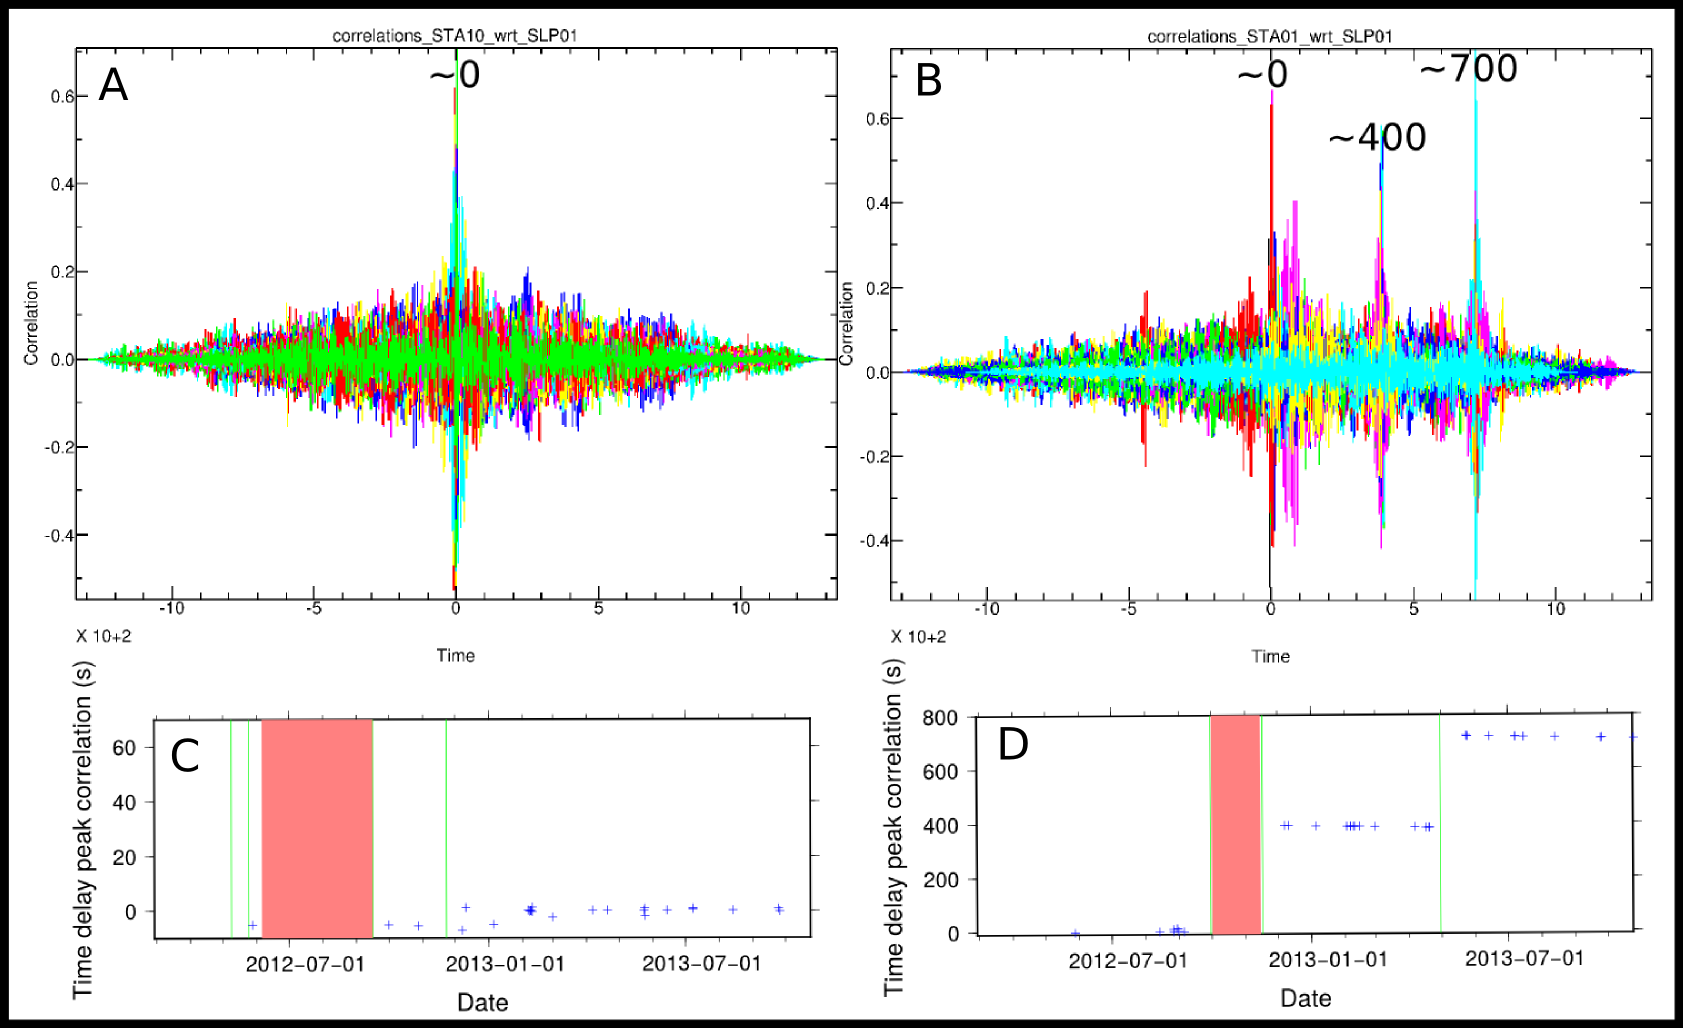
\includegraphics[scale=0.4]{Figs/correlacao_tempo_de_chegada_resultado.png}
\caption[Correlação de eventos sucessivos de fontes sísmicas entre duas estações sismográficas]{Correlação de eventos sucessivos de fontes sísmicas entre as estações sismográficas STA10 e SLP01 (A) e  STA01 e SLP01 (B). Na parte inferior mostram o atraso do tempo de chegada da onda P da correlação pelo tempo. As retas verticais verdes mostram os períodos onde teve manutenção do equipamento e as em vermelhas quando a estação não estava funcionando (C e D).}
\label{teste_tempo_results}
\end{figure}

Os gráficos gerados com a correlação são vistos na Figura \ref{teste_tempo_results}. Os resultados mostram que para algumas estações temporárias há erros na chegada da onda P, como visto na Figura \ref{teste_tempo_results}-B. Tais erros podem ter sidos gerados por difentes fatores, como erro no sinal do GPS acoplado à estação, erro instrumental, mas ainda não foi identificado o que causou este erro. Na Figura \ref{teste_tempo_results}-C e D encontramos um gráfico mostrando o tempo de atraso das correlações pelo tempo. As linhas verticais(verdes) nos gráficos mostram intervalos onde foram feitas manutenções nas estações temporárias. Vemos que na Figura \ref{teste_tempo_results}-D, que após as manutenções na estação STA01, erros sistemáticos apareceram nos registro e isso pode ser confirmado na Figura \ref{teste_tempo_results}-B.

Com esse tratamento preliminar dos dados pôde-se selecionar melhor o banco de dados e tentar minimizar os erros gerados no processamento da dispersão das curvas de superfície. Após estes estudos, as estações temporárias STA23 e STA24 foram consideradas impróprias para o cálculos da dispersão das ondas Rayleigh. Porém serão aproveitadas quando for analisada a dispersão das ondas Love, pois as componentes horizontais estão boas. A estação STA22 só possui 4 dias de dados registrados, logo foi descartada da análise.

\chapter{Função do Receptor}
\today

\section{Introdução}

No ínicio desse trabalho somente os dados de eventos incluídos no catálogo do IRIS (\textit{Incorporated Research Institutions for Seismology}) com magnitude maior que 5,5 entre maio de 2011 e maio de 2012 foram utilizados. Porém agora utiliza-se dados coletados na rede Sismográfica, mostrada na \ref{map_loc}, até o fim do segundo semestre de 2013. A Figura \ref{mapa_eventos} mostra eventos sísmicos registrados na estação STA08 mostrando a delimitação dos eventos pela distância epicentral, além de mostrar sismos com magnitude maior que 5.5 mb.

O sismômetro registra pequenas variações horizontais e verticais de amplitude das partículas do terreno na escala microscópica ao longo das direções Vertical (Z), Norte-Sul (N) e Leste-Oeste (E), chamado sistema ZNE, como observado na Figura \ref{simograma}. No entanto, o sinal bruto nas direções ZNE não está alinhado aos eixos de propagação das ondas geradas pelo sismo, logo a resposta em cada componente mostra uma sobreposição de vários tipos de ondas. Com a finalidade de isolar a contribuição de cada onda registrada nos dados, o sistema de coordenadas dos registros são rotacionadas, através do SAC (\textit{Seismic Analysis Code}), para se alinharem com os eixos de propagação das ondas através da seguinte matriz de rotação:

\begin{eqnarray}
 & & \left[ \begin{array}{c} R \\ T \\ Z \end{array} \right] = \begin{bmatrix} \cos \theta & \sin \theta & 0 \\ - \sin \theta & \cos \theta & 0 \\ 0 & 0 & 1 \end{bmatrix} \left[ \begin{array}{c} E \\ N \\ Z \end{array} \right]
\label{rotacao}
\end{eqnarray}

O resultado da equação \ref{rotacao} discrimina claramente a contribuição de cada componente  no sismograma. A componente N (norte-sul) transforma-se na componente T (transversal) e guarda os registro da componente horizontal da onda S, chamada de onda SH. A resposta da onda SV é resgistrada na componente radial do sismograma, chamada R, como pode ser visualizada na Figura \ref{sismo_radial}.

\begin{figure}[!ht]
\centering
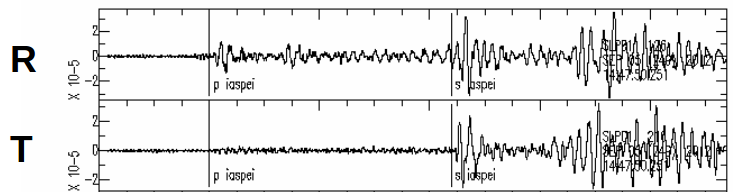
\includegraphics[scale=0.6]{Figs/Componente_Radial_Transversal.png}
\caption{Sismograma mostrando as componentes Radial e Transversal.}
\label{sismo_radial}
\end{figure}

\section{Processamento}

Para o cálculo a espessura crustal na região utilizou-se o método da Função do Receptor, que foi desenvolvido por \cite{Langston_1977}. O programa SAC (\textit{Seismic Analysis Code}) foi usado para fazer o processamento e o cálculo das Funções Receptores. Tal método faz uso do sinal de tele-sismos, geradores de ondas planas de incidência quase-vertical embaixo de uma dada estação. A onda P incide na discontinuidade de Mohorovicic e se decompõe em uma onda P transmitida e uma onda S convertida. A diferença do tempo de chegada das duas ondas, onda S tem velocidade inferior a onda P, e de outras reflexões permite inferir a profundidade da discontinuidade de Mohorovicic, também chamada de Moho, como mostrado na Figura \ref{funcoes_sinteticas} .

\begin{figure}[!ht]
\centering
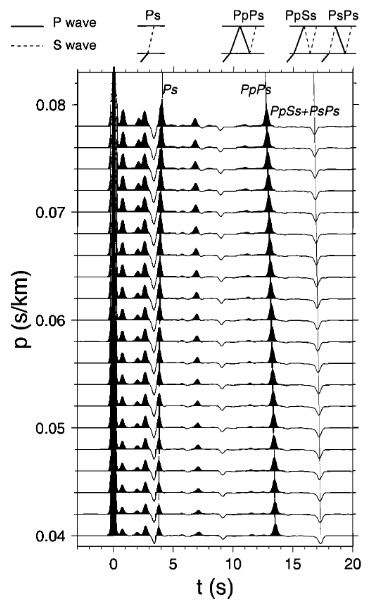
\includegraphics[scale=0.8]{Figs/funcoes_sinteticas.png}
\caption[Funções do Receptor em função do parâmetro do raio para o Modelo de Velocidade Padrão do Sul da Califórnia.]{Funções do Receptor em função do parâmetro do raio para o Modelo de Velocidade Padrão do Sul da Califórnia, em \cite{Zhu_Kanamori_2000}. A fase Ps convertida em Moho e suas múltiplas  PpPs, PpSs, e PsPs e seus traços são ilustrados no topo da imagem. Outras reflexões não-rotuladas são as conversões P-S em 5.5 km e 16 km, discontinuidades intracrustais no modelo.}
\label{funcoes_sinteticas}
\end{figure}

Para uma estimativa precisa das Funções do Receptor é essencial que o tempo de chegada da onda P seja determinado com baixa incerteza. Então os dados foram examinados visualmente para registrar o tempo de chegada da onda P direta. 

As Funções do Receptor são calculadas com uma deconvolução componente radial (R) pela componente vertical (Z), como é mostrado por \cite{clayton_source_1976}, \cite{Langston_1977}, \cite{ammon_isolation_1991}, \cite{cassidy_numerical_1992}, \cite{Zhu_Kanamori_2000}. Essa operação remove efetivamente a resposta instrumental, a assinatura da fonte e a propagação da fonte até Moho. E o sinal resultante é a assinatura da propagação próxima à estação. Então a Função do Receptor é sensível na delimitação da estruturação superficial da crosta embaixo da estação.

Computar as Funções do Receptor é um problema de deconvolução,  \cite{ligorria_iterative_1999}. \cite{langston_structure_1979} descreve a resposta do deslocamento teórico para uma onda plana P incidindo sobre uma empilhamento de interfaces horizontais ou inclinadas no domínio do tempo pode ser dada por:

\begin{eqnarray} \label{lang_equacao}
D_{V}(t) = I(t) * S(t) * E_{V}(t)
\nonumber
\\
D_{R}(t) = I(t) * S(t) * E_{R}(t)
\\
\nonumber
D_{T}(t) = I(t) * S(t) * E_{T}(t)
\end{eqnarray}

Onde $S(t)$ é a resposta efetiva da fonte em função do tempo de uma onda incidente, $I(t)$ é a resposta do impulso instrumental e $E_{V}(t)$, $E_{R}(t)$ e $E_{T}(t)$ são as respostas do impulso da estruturua vertical, radial e tangencial, respectivamente. A componente $S(t)$ pode ser muito complicada de ser computada, pois ela é relacionada a história do deslocamento no tempo e reverberações na aŕea da fonte.

\cite{langston_structure_1979} assume que eventos profundos observados em dados telessísmicos, na componente vertical do movimento do terreno ($D_{V}(t)$), se comportam como um pulso em função do tempo convoluído com a resposta instrumental e com chegadas tardias menores. Cálculos teóricos para estruturas crustais mostram que reverberações crustais e fases convertidas na componente vertical de ondas P são menores. Então se aproxima:

\begin{eqnarray} \label{lang_suposicao}
I(t) * S(t) \simeq D_{V}(t)
\end{eqnarray}

\cite{langston_structure_1979} faz uma suposição implícita que $D_{V}(t)$ comporta-se como uma função delta de Dirac, como pode ser observado na equação \ref{lang_suposicao}. Assumindo que a resposta instrumental é compensada entre as componentes, $E_{R}(t)$ e $E_{T}(t)$ podem ser encontrados passando para o domínio da frequência a equação \ref{lang_equacao} e fazendo as seguintes deconvoluções:

\begin{eqnarray} \label{lang_resposta}
E_{R}(\omega) =  \frac{D_{R}(\omega)}{I(\omega)S(\omega)} \simeq \frac{D_{R}(\omega)}{D_{V}(\omega)}
\\ \nonumber
E_{T}(\omega) =  \frac{D_{T}(\omega)}{I(\omega)S(\omega)} \simeq \frac{D_{T}(\omega)}{D_{V}(\omega)}
\end{eqnarray}

$E_{R}(t)$ e $E_{T}(t)$ são retransformadas para o domínio do tempo, importante lembrar que nessa técnica a informação da fase é conservada. \cite{langston_structure_1979} resalta que o resultado da série temporal pode ser interpretado diretamente com um sismograma, permitindo que tempo e amplitude de chegadas possam ser examinadas de uma maneira inequívoca.

\cite{clayton_source_1976}, \cite{langston_structure_1979}, \cite{ligorria_iterative_1999} mostram que o processo de deconvolução possui um instabilidade numérica devido a vários fatores, como o ruído aleatório contido nos dados e a limitação da banda de frequência. Para acabar com os problemas gerados na deconvolução, \cite{clayton_source_1976} introduz um nível de amplitude mínimo permitido da fonte, nomeado de \textit{water-level}, como pode ser visto na Figura Figura \ref{water_level}. Faz-se isso para reduzir componentes de ruídos espúrios e efeitos de pequenos erros na estimação da fonte. Na deconvolução \textit{water-level} a maneira de se evitar a divisão por números pequenos é substituir esses valores pequenos no denominador por uma fração do valor máximo do denominador (para todas as frequências), tal fração é chamada de parâmetro de \textit{water-level}, segundo \cite{Ammon_waterlevel_1997}. \textit{water-level} pode agir, em alguns casos, como um filtro "passa-baixa", "passa-alta" e "não-passa", como mostrado na Figura \ref{water_level} .

\begin{figure}[!ht]
\centering
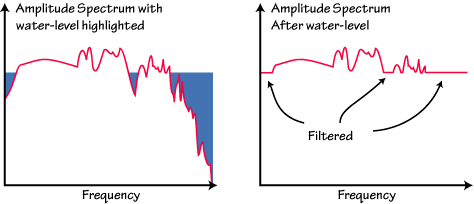
\includegraphics[scale=0.8]{Figs/water_level.png}
\caption{Gráficos mostrando o funcionamento do \textit{water-level}, segundo \cite{Ammon_waterlevel_1997}.}
\label{water_level}
\end{figure}

No processamento dos dados a deconvolução no domínio do tempo feita é de acordo com a teoria criada por \cite{ligorria_iterative_1999}, esta é nomeada de deconvolução interativa. Tal método segue a ideia de \cite{kikuchi_inversion_1982}, que é usado para estimar funções do tempo de fontes de grandes terremotos. A deconvolução interativa de  \cite{ligorria_iterative_1999} minimiza através do método dos mínimos quadrados a diferença entre o sismograma horizontal observado e um sinal predito pela convolução de um conjunto de picos atualizados interativamente com a componente vertical do sismograma.

\begin{figure}[!ht]
\centering
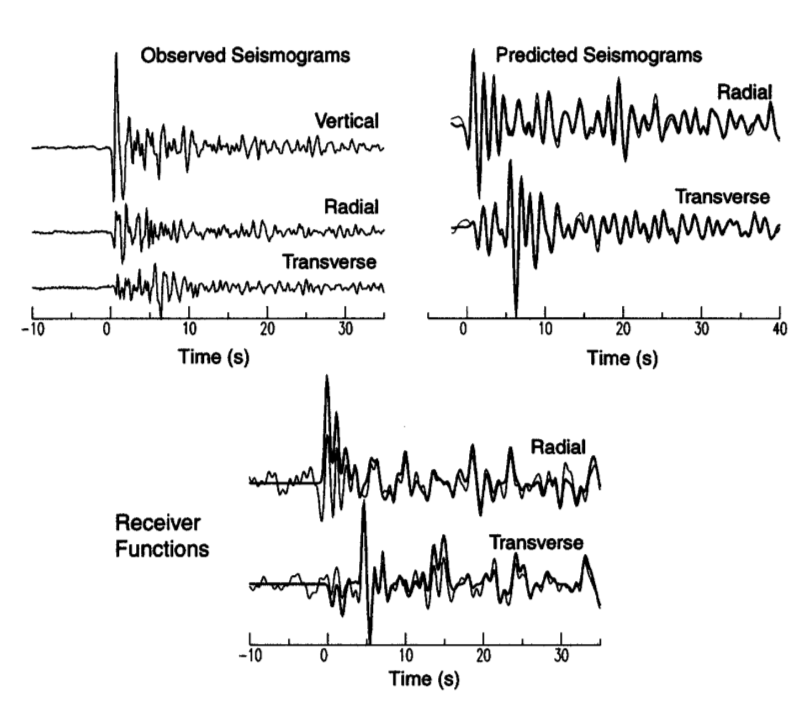
\includegraphics[scale=0.5]{Figs/deconvolucao_interativa.png}
\caption[Estimando a Função do Receptor utilizando pequenos períodos.]{Estimando a Função do Receptor utilizando pequenos períodos. Os sinais originais são mostrados na parte superior esquerda, as funções do Receptor calculadas utilizando \textit{water-level} são comparadas com o método interativo no painel inferior. Os sinais horizontais preditos são comparados com os sinais horizontais observados no painel superior direito. \citep{ligorria_iterative_1999}.}
\label{deconvolucao_interativa}
\end{figure}

\section{Pós-processamento}

Após gerar sismogramas pela deconvolução Interativa, as séries temporais passaram por um processo de triagem para qualificar as que obtveram melhor resultado. Tal seleção foi feita sob um critério visual observando as funções do receptor que respeitam o formato determinado por \citep{langston_structure_1979}.

Tendo como objetivo a análise da estrutura da crosta, buscou-se inicialmente o cálculo da profundidade de Moho, um importante parâmetro porque é relacionada à geologia e a evolução tectônica da região. \cite{Zhu_Kanamori_2000} propõe um método robusto utilizando a análise das Funções do Receptor para calcular a profundidade de Moho.

Com um modelo da estrutura da Terra, neste caso o IASPEI 91 em \cite{kennet_iaspei_1991}, utiliza as velocidades medianas na crosta para calcular as diferenças de tempo teórica entre a onda P direta e a onda P convertida em S, bem como os tempos das outras reverberações na crosta. De posse de uma dada velocidade $v_{P}$, os tempos de chegada podem ser calculados usando a profundidade de Moho ($H$), a razão $v_{P}$/$v_{S}$ e o parâmetro do raio ($p$), dependente da localização do evento e da profundidade, do modelo.

\cite{Zhu_Kanamori_2000} mostra que os tempos teóricos entre $P_{S}$ e P podem ser utilizados para estimar a espessura crustal, dado uma velocidade crustal média:

\begin{eqnarray}
H = {\frac{t_{P_{s}}}{{\sqrt{\frac{1}{V_{s}^{2}} - p^{2}}} - \sqrt{\frac{1}{V_{p}^{2}} - p^{2}}}}
\end{eqnarray}

E o erro pode ser dado por:

\begin{eqnarray}
\Delta H = \frac{\partial H}{\partial V_{p}} \Delta V_{p}
\end{eqnarray}

Porém a dependência de $t_{Ps}$ em relação a $V_{p}$ não é tão forte quanto a $V_{s}$, especificamente à razão $V_{p}/V_{s}$, $\kappa$. Logo o erro e quantificado:

\begin{eqnarray}
\Delta H = \frac{\partial H}{\partial \kappa } \Delta \kappa 
\end{eqnarray}

\cite{Zhu_Kanamori_2000} demonstra que uma variação de 0.1 na razão $v_{P}$/$v_{S}$ pode acarretar erros de aproximadamente 4 km na espessura crustal. Essa ambiguidade pode ser reduzida utilizando as outras fases, reverberações, da onda P. Tais fases provém informações adicionais, como mostrado nas equações abaixo:

\begin{eqnarray}
H = {\frac{t_{P_{p}P_{s}}}{{\sqrt{\frac{1}{V_{s}^{2}} - p^{2}}} + \sqrt{\frac{1}{V_{p}^{2}} - p^{2}}}}
\end{eqnarray}

\begin{eqnarray}
H = \frac{t_{P_{p}P_{s}+P_{s}P_{s}}}{{2\sqrt{\frac{1}{V_{s}^{2}}- p^{2}}}}
\end{eqnarray}

Em situações reais, identificar a $P_{s}$ em Moho e as múltiplas e medir seus tempos de chegada em um único traço da função do receptor pode ser muito difícil devido ao ruído de fundo, espalhamento devido a heterogeneidades crustais e conversões P para S de outras discontinuidades de velocidades.

Para aumentar a razão sinal/ruído empilha-se as funções do receptor de multiplos eventos. Esse empilhamento é feito no domínio do tempo para um aglomerado de eventos. \cite{Zhu_Kanamori_2000} define um empilhamento $H$-$\kappa$ como:

\begin{eqnarray} \label{Hk_stack}
s(H,\kappa) = \omega_{1}r(t_{1}) + \omega_{2}r(t_{2}) + \omega_{3}r(t_{3})
\end{eqnarray}

onde $r(t)$ é a função do receptor radial, $t_{1}$, $t_{2}$ e $t_{3}$ são os tempos de chegada preditos  $t_{s}$,  $t_{P_{p}P_{s}}$ e  $t_{P_{p}P_{s}+P_{s}P_{s}}$ correspondente a uma espessura crustal $H$ e a uma razão $V_{p}/V_{s}$ e $\omega_{i}$ são os pesos dos fatores, e $\sum \omega_{i} = 1$. 

\begin{figure}[!ht]
\centering
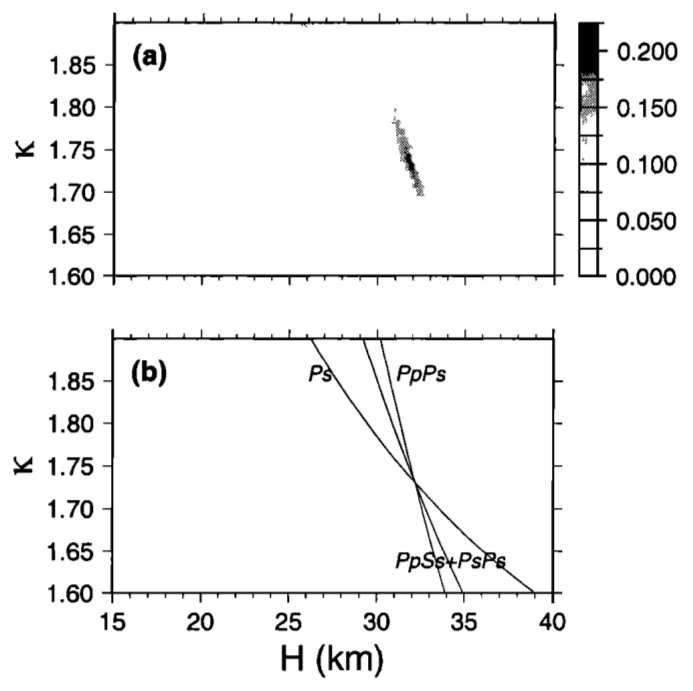
\includegraphics[scale=0.5]{Figs/grid_search.png}
\caption[a) $s(H,\kappa)$ do empilhamento das funções do receptor utilizando a equação \ref{Hk_stack}.b) Relações $H-\kappa$ para diferentes fases convertidas em Moho.]{a) $s(H,\kappa)$ do empilhamento das funções do receptor utilizando a equação \ref{Hk_stack} . Ela encontra o ponto máximo quando se usa uma espessura crustal $H$ e uma razão $v_{P}$/$v_{S}$ coerentes. b) Relações $H-\kappa$ para diferentes fases convertidas em Moho. Cada curva representa a contribuição dessa fase convertida ao empilhamento, segundo \cite{Zhu_Kanamori_2000}.}
\label{grid_search}
\end{figure}

Ao invés de tentar ajustar toda a função, o método faz uma pesquisa, \textit{grid search}, da espessura crustal e da razão $v_{P}$/$v_{S}$ para calcular o tempo de chegada teórico das ondas P convertidas em S e das múltiplas para cada registro. A melhor combinação da espessura crustal e da razão $v_{P}$/$v_{S}$, $\kappa$, é aquela que maximiza o valor das amplitudes reais das funções receptor, como pode ser visualizado na Figura \ref{grid_search}.

As incertezas na medidas, mostradas na Tabela \ref{tabela1}, estão diretamente ligadas a quantidade e qualidade das Funções do Receptor. A seleção das melhores Funções do Receptor é um fase importante, pois a qualidade da Função do Receptor é prepoderante sobre a quantidade. A imprecisão associada a cada um dos parâmetros obtidos pelo método de \cite{Zhu_Kanamori_2000} é estimada pelo método "\textit{bootstrap}", desenvolvido por \cite{efron_statistical_1991}.

O método "\textit{bootstrap}" gera do conjunto de Funções do Receptor subconjuntos contendo traços selecionados aleatoriamente. Esse método é repetido para cada subconjunto, resultando num conjunto de parâmetros de $H$ (profundidade de Moho) e de razão $v_{p}/v_{s}$. A média e o desvio padrão dos valores provém um valor médio e uma estimativa da incerteza associada ao cálculo. Não existe uma regra para determinar o número de subconjuntos que precisam ser gerados, o crucial é a busca por um valor que faça a estimativa estabilizar, incluindo as incertezas. Em geral usa-se um valor entre 100 e 200 subconjuntos dependendo da quantidade de traços disponíveis durante o "\textit{bootstrap}".

\cite{assumpcao_crustal_2002},\cite{sand_franca_crustal_2004} e \cite{julia_deep_2008} mostram a necessidade de um cuidado especial ao empilhar as Funções do Receptor, pois há uma dependência azimutal  e com isso um deslocamento das reflexões de Moho. Isso pode ser observado na Figura \ref{tauptime}. A solução foi a a separação das funções do receptor de acordo com o backazimute e parâmetro do raio. 

\begin{figure}[!ht]
\centering
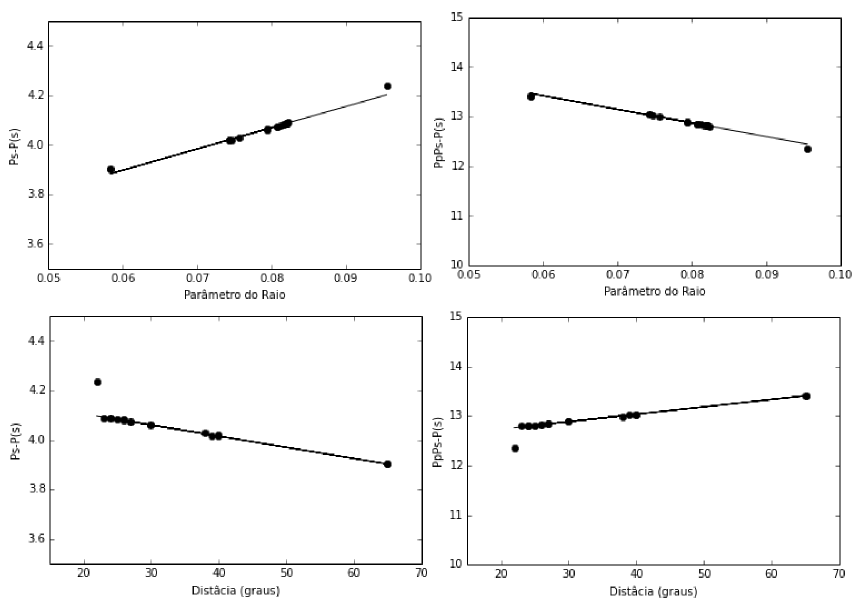
\includegraphics[scale=0.7]{Figs/tempo_teorico_modelo_tauptime.png}
\caption[Tempos teóricos para a reflexão $Ps$ (gráficos à esquerda) e fases $PpPs$ segundo o modelo de \cite{kennet_iaspei_1991}.]{Tempos teóricos para a reflexão $Ps$ (gráficos à esquerda) e fases $PpPs$ segundo o modelo de \cite{kennet_iaspei_1991}. Os tempos estão classificados segundo o parâmetro do raio e as distâncias epicentrais.}
\label{tauptime}
\end{figure}

Para a separação azimutal levou-se em conta a sismicidade ao redor da região. Visto isso, fez-se uma separação em quatro quadrantes: NE, SE, SW e NW. Cada quadrante representa um agloramedo de eventos, estes aglomerados variam em magnitude e em quantidade, como pode ser observado na Figura \ref{map_loc}. 

Os eventos oriundos da parte nordeste(NE) são escassos e as principais fontes são a Cadeia Meso-atlântica e a cordilheira Alpina na Europa. Já os sismos do sudeste(SE) são originários das Ilhas South Georgia e SouthSandwhich, localizadas no Atlântico Sul, e do Sul da África. A sudoeste é marcante a presença de eventos Andinos, provenientes do Chile e Argentina, e de eventos do Oceano Pacífico. Assim como a sudoeste, os eventos vindos a noroeste(NW) da área são Andinos, oriundo do norte do Chile e do Peru. Também é marcante eventos da América Central,México e Califórnia, estes são bem visíveis na Figura \ref{map_loc}.

O tipo de método utilizado no empilhamento do sinal permite recuperar informações com qualidade e confiabilidade das Funções do Receptor. O empilhamento linear do sinal separado pelo azimute ainda contém um nível de ruído aleatório que não é eliminado pela soma do sinal devido a fatores como a qualidade dos dados, distribuição azimutal dos eventos,\cite{schimmel_noise_1997}. Para isso utilizou-se o Empilhamento Ponderado pela Fase, \textit{Phase Weight Stack (PWS)} , prosposto por \cite{schimmel_noise_1997} como uma ferramenta para reduzir o ruído  incoerente contido no dado, como observado na Figura \ref{empilhamento}-b). Este método concebido por \cite{schimmel_noise_1997} se torna eficiente por conseguir recuperar algumas reflexões coerentes em meio ao ruído, mesmo apresentando uma alteração na forma do sinal. 

Com a finalidade de suprimir este ruído que não é coerente, utiliza-se o empilhamento da fase do sinal como uma medida de coerência para a soma dos traços sísmicos. A ideia consiste em usar o empilhameto da fase como um peso dependente do tempo do empilhamento linear do sinal sísmico. Isto é facilmente realizado pela multiplicação dos empilhamento da fase com o empilhamento linear do sinal, como observa-se na equação \ref{PWS}.

\begin{equation}
\label{PWS}
g(t) = \frac{1}{N} \sum_{j=1}^{N}s_{j}(t)\left | \frac{1}{N} \sum_{k=1}^{N}exp\left [ i\Phi _{k}(t) \right ]  \right |^{v}
\end{equation}

onde $N$ é o número de traços, $s(t)$ o traço sísmico, $\Phi (t)$ a fase e $v$ a potência. 

Segundo \cite{schimmel_noise_1997} . cada amostra do empilhamento linear será ponderado pela coerência de suas fases instantâneas. O empilhamento da fase funciona como um filtro com uma certa nitidez da transição entre a semelhança e dessemelhança da fase, que é
controlados pela potência $v$. 

Este trabalho incrementa a metodologia idealizada por \cite{schimmel_noise_1997}, pois os traços utilizados para calcular a fase do sinal foram janelados previamente. \cite{harris_use_1978} mostra que a performance da transformada discreta de Fourier em dados janelados é mais eficiente. Com o janelamento pré-PWS o resultado gerado consegue, além de reduzir o ruído incoerente, recuperar outras reflexões que não eram bem observadas no resultado gerado pelo PWS, como pode ser observado na Figura \ref{PWS}-c), devido a baixa qualidade das funções do receptor.

\begin{figure}[!ht]
\centering
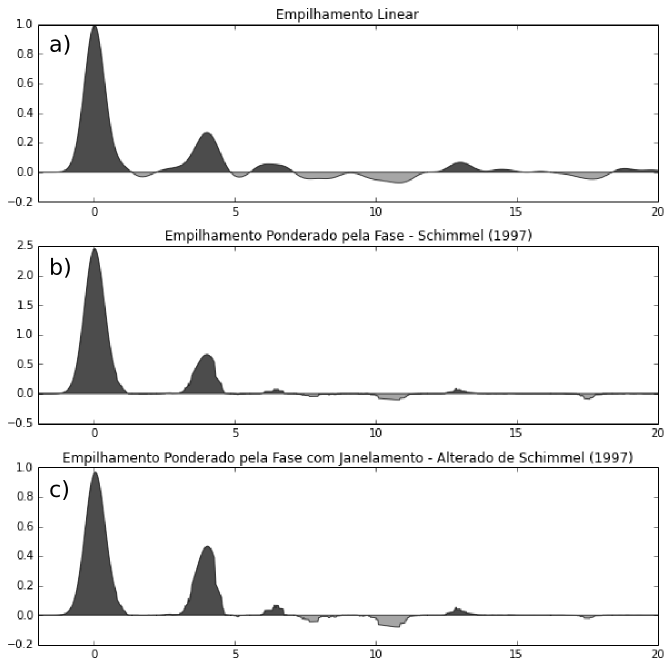
\includegraphics[scale=0.8]{Figs/empilhamento.png}
\caption[Comparação entre os tipos de empilhamento utilizados nas Funções do Receptor.]{Comparação entre os tipos de empilhamento utilizados nas Funções do Receptor. a) Empilhamento linear das funções do receptor separadas pelo azimute na estação SLP01. b)  Empilhamento das funções do receptor ponderado pela fase proposto por \cite{schimmel_noise_1997}. c) Empilhamento das funções do receptor ponderado pela fase com janelamento do sinal}
\label{empilhamento}
\end{figure}

\section{Modelagem das Funções do Receptor}

A caracterização do arcabouço estrutural utilizando métodos sismológicos possui problemas de unicidade de solução, como outros métodos geofísicos.  Essa falta de informação direta do objeto em estudo proporciona uma gama de soluções, entretante há inúmeros meios de se contornar essa situação. A modelagem mostra-se uma boa opção, pois consegue comprovar se a técnica utilizada tem resolução para seu objetivo.

\begin{figure}[!ht]
\centering
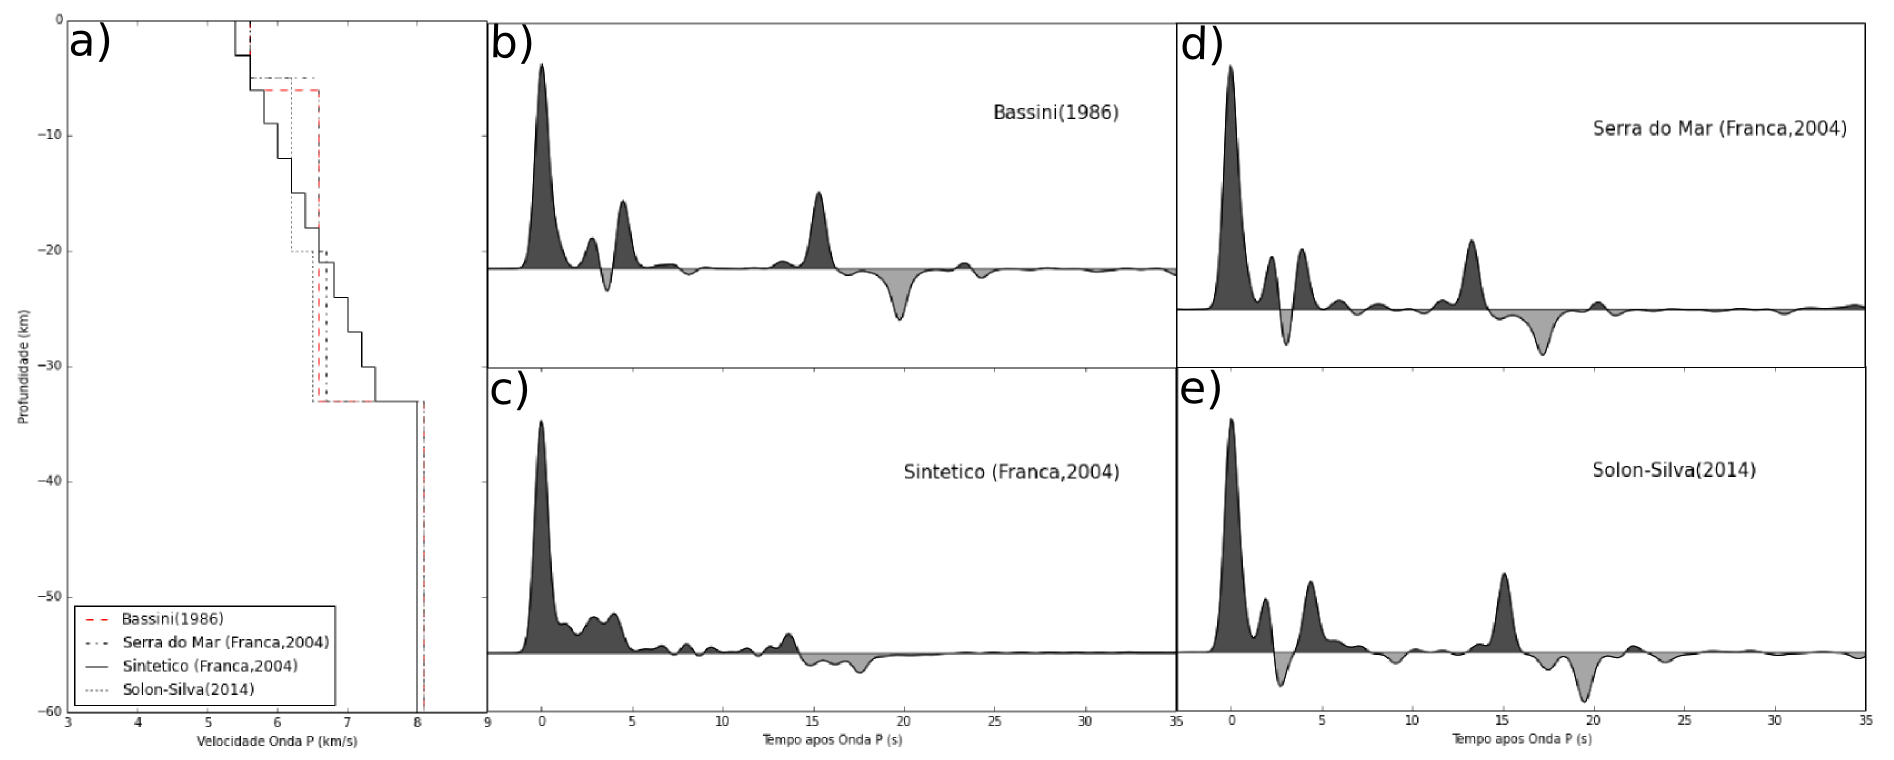
\includegraphics[scale=0.25]{Figs/modelagem_RF.png}
\caption{Funções do Receptor Sintéticas para área abrangida pelo projeto do SUBSAL segundo vários tipos de modelos de velocidade da onda P.}
\label{modelagem}
\end{figure}

Para delimitar as principais feições estruturais da área em estudo fez o uso de modelos simples, como visto na Figura \ref{modelagem}-a, apenas com camadas planas, porém tais modelos são condizentes com o contexto geológico local. Com esses modelos pretende-se mostrar que as estimativas da espessura crustal e razão $V_{p}/V_{s}$ são consistentes com os dados observados. Para a confecção e cálculo das Funções do Receptor Sintéticas aplicou-se a metodologia proposta por \cite{Ammon_waterlevel_1997}. 

Os programas utilizados para criar os modelos de velocidade da onda $P$ foram "\textit{icmod}" e "\textit{vplot[s]}". A preparação dos dados sintéticos foi feita pelo programa "\textit{respknt}". O programa "\textit{pwaveqn}" calculou as Funções do Receptor no domínio da frequência para os modelos pré-estabelecidos. Os parâmetros utilizados para o cálculo das Funções do Receptor estão na Figura \ref{modelagem}. Toda a demonstração da modelagem e cálculo das Funções do Receptor sintéticas está disponibilizada por \cite{Ammon_waterlevel_1997} em \url{http://eqseis.geosc.psu.edu/~cammon/HTML/RftnDocs/rftn01.html}.

Os modelos de velocidade da onda P ($V_{p}$) são exemplos retirados da literatura sobre a região em estudo, \ref{modelagem}-a). \cite{Bassini_1986} foi o primeiro a estimar a estrutura crustual para a região da Faixa Riberia, então neste trabalho utilizou-se o modelo de velocidade sísmica para a região da Serra do Mar, como observado na Figura \ref{modelagem}-b). Mais tarde, \cite{sand_franca_crustal_2004} re-compilou os dados de \cite{Bassini_1986} e propôs um novo modelo de velocidade sísmica da região da Serra do Mar, como visto na Figura \ref{modelagem}-d). Recentemente \cite{flora_solon_ancient_2013} e \cite{Silva_2014} geraram resultados da estrutura crustal reginal através dos métodos magnetométrico e gravimétrico, respectivamente. Baseando-se nesses resultados, organizou-se um modelo de velocidade sísmica para a região em estudo, como visto na Figura \ref{modelagem}-e). Uma outra opção de modelo sísmico levantada por \cite{sand_franca_crustal_2004} é o modelo Sintético, mostrado na Figura \ref{modelagem}-c). Neste modelo o autor considera que a variação das propriedades físicas da região aumenta progressivamente com a profundidade.

\begin{figure}[!ht]
\centering
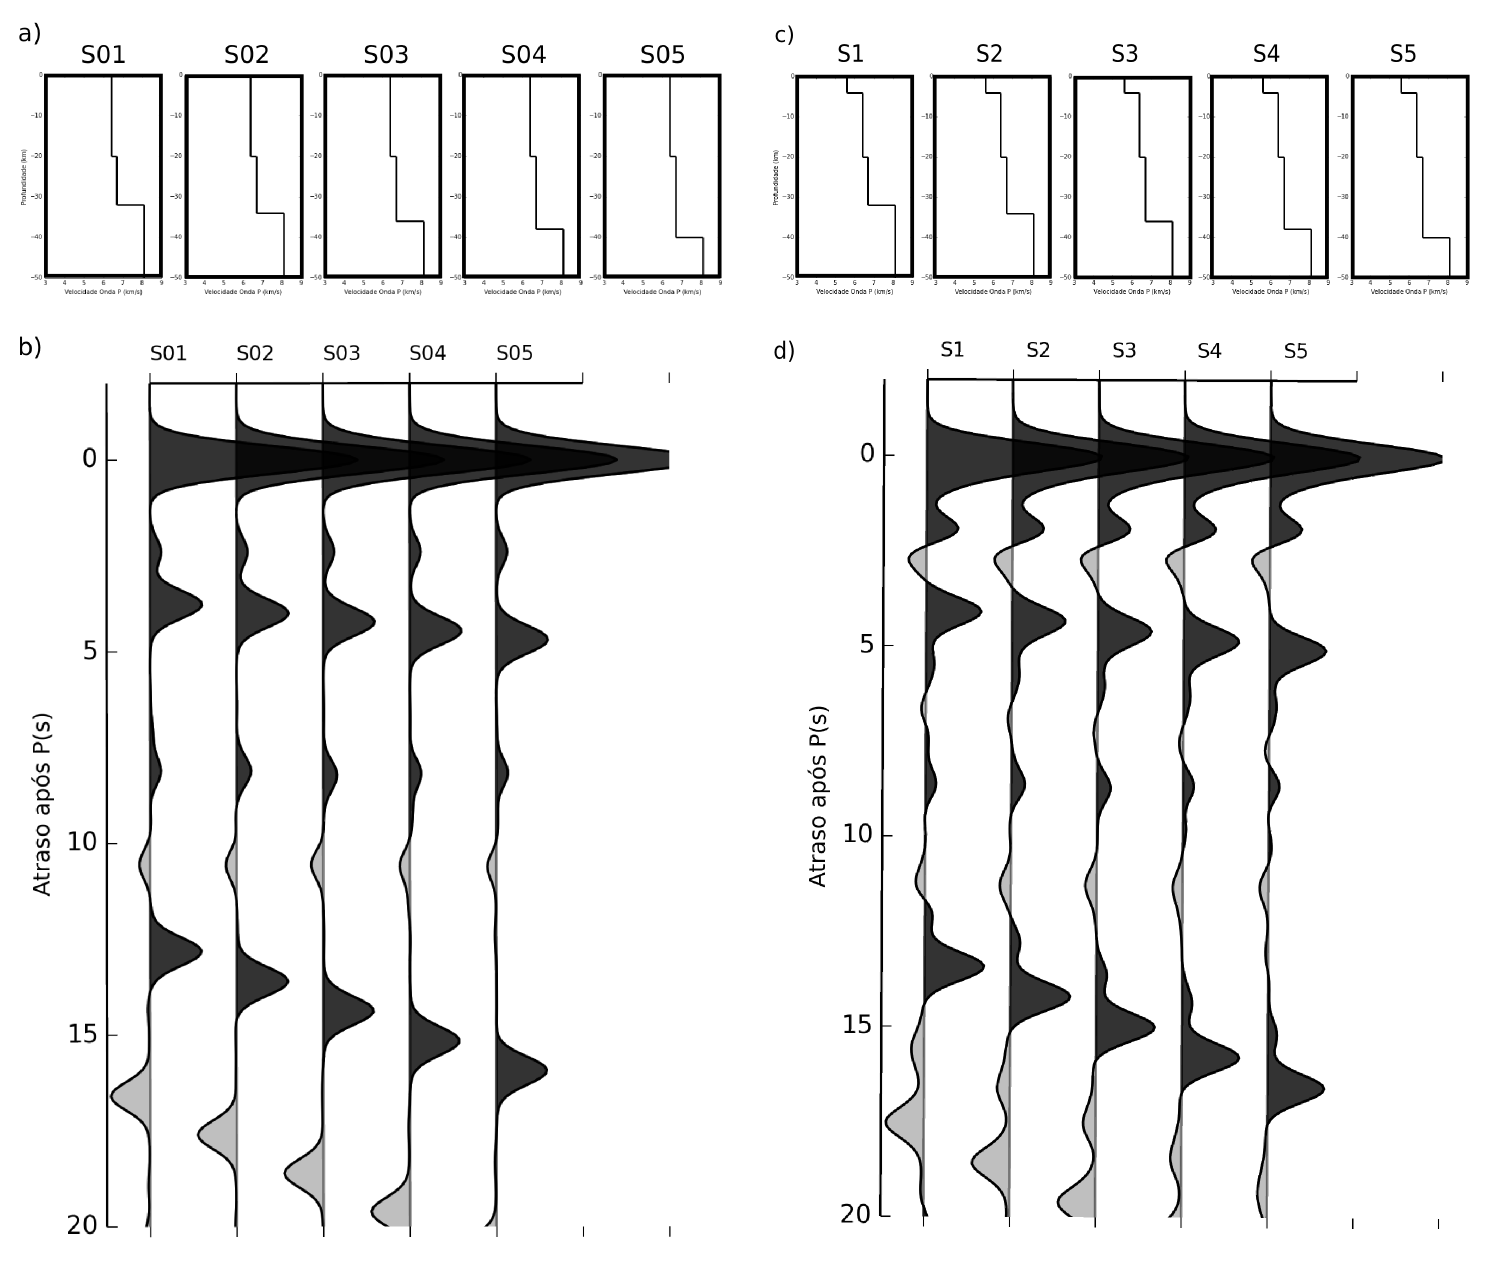
\includegraphics[scale=0.25]{Figs/perfil_RF_sintetico.png}
\caption{Perfil com Funções do Receptor Sintéticas para área abrangida pelo projeto do SUBSAL segundo modelos de velocidade Solon-Silva(2014), como mostrado na Figura \ref{modelagem}.}
\label{perfil_modelagem}
\end{figure}

As Funções do Receptor sintéticas apresentadas na Figura \ref{modelagem} mostram uma reflexão característica por volta de 5 segundos, está é a primeira reflexão de Moho, onde a onda P se converte em S. Antes dessa reflexão é notável um pulso senoidal em torno de 2.5 segundos nas Figuras \ref{modelagem}-b), \ref{modelagem}-d) e \ref{modelagem}-e). Este pulso está relacionado com a camada superficial de baixa velocidade. Tal camada possui espessura aproximada de 5 quilômetros, esta é análoga a uma bacia sedimentar, no contexto local pode ser representada como a Bacia de Taubaté na região da Faixa Ribeira. As outras reverberações são bem características, As multiplas $PpPs$ e $PpSs+PsPs$ são bem demarcadas em $\sim 13$ e $\sim 19$ segundos, respectivamente.

Na Figura \ref{perfil_modelagem} observa-se três perfis de modelos com velocidades diferentes. Tais modelos foram confeccionados de acordo com o modelos geológicos locais e com os perfis de velocidades citados anteriormente. A Figura \ref{perfil_modelagem}-a) mostra os perfis de velocidade baseados nas inversões de \cite{flora_solon_ancient_2013} e de \cite{Silva_2014} com uma discontinuidade constante bem marcada no meio da crosta, por volta de $20 \sim km$. A resposta dessa discontinuidade média da crosta é apresentada na Figura \ref{perfil_modelagem}-b). Onde também é mostrado uma discontinuidade de Moho mergulhante, bem marcada pela distância entre a primeira reflexão e a segunda grande reflexão, conversão da onda P em S.

Nos modelos de velocidade apresentados na Figura \ref{perfil_modelagem}-c) é adicionado uma camada com baixa velocidade na parte superior do perfil, de profundidade $5 km$, analogamente à bacias sedimentares terciárias presentes na área, como a Bacia de Taubaté. A resposta a essa camada de baixa velocidade é mostrada na Figura \ref{perfil_modelagem}-c) como um sinal senoidal por volta de 2,5 segundos.

Na Figura \ref{perfil_modelagem}-e) adicionou-se ao modelo de velocidade uma velocidade alta na parte superior da crosta com inclinação contrária a discontinuidade caracterizada com Moho. Nota-se na Figura \ref{perfil_modelagem}-f) que há uma sobreposição de sinais referentes a essas essa discontinuidades. Logo quanto maior a complexidade da área há uma dificuldade na obtenção de resultados claros pela Funções do Receptor.

\pagebreak
\chapter{Correlação Cruzada de Ruído Ambiental Sísmico}

\section{Introdução}

Os métodos para determinar a estrutura sísmica da Terra, em particular os métodos tomográficos, baseiam-se num princípio simples: a determinação das velocidades de propagação das ondas sísmicas e a procura de um modelo que melhor se ajuste às velocidades encontradas. A resolução dos modelos obtidos depende do tipo de onda utilizado e da geometria espacial das estações sismográficas segundo à fonte do sinal. \cite{aki_space_1957} propôs a utilização do ruído sísmico ambiental para medir a dispersão das ondas Rayleigh e Love nas camadas mais superficiais. Somente \cite{campillo_long-range_2003}  e \cite{shapiro_emergence_2004} mostraram, pela primeira vez, a  presença de ondas superficiais nas correlações cruzadas entre pares de estações.

\cite{campillo_long-range_2003}, \cite{shapiro_emergence_2004} e, principalmente, \cite{wapenaar_retrieving_2004} mostram que pode-se recuperar a resposta elástica da Terra a partir da correlação cruzada entre dois pontos em  um campo de ondas difuso ou aleatório. Essa resposta é aproximada como a Função de Green, como é mostrada na equação \ref{crosscorrelation}. 

\cite{boschi_measuring_2013} define a correlação cruzada ($C_{xy}(t,\omega)$) como: 
\begin{eqnarray}
\label{crosscorrelation}
C_{xy}(t,\omega) = \frac{1}{2\pi}\int_{-T}^{T}u_{1}(x,t,\omega)u_{2}(y,t+\tau,\omega) d\tau
\end{eqnarray}

onde $u_{1}$ e $u_{2}$ são sinais registrados em duas estações nas posições $x$ e $y$, $t$ é o tempo, $\omega$ é a frequência, $\tau$ é o atraso e o parâmetro $T$ define o tamanho da janela em que a correlação cruzada é computada.
\\

Por possuir inúmeras vantagens em relação aos métodos de análise tradicionais que utilizam dados de sismos para a tomografia sísmica, o número de artigos sobre a correlação de ruído ambiental cresceu bastante. \cite{shapiro_emergence_2004} lista as seguintes vantagens: as medidas podem ser realizadas em qualquer direção de propagação e não estão limitadas à geometria fonte-receptor; não dependem da localização da fonte; a zona de sensibilidade destas medições situa-se na região entre as duas estações; pode-se analisar pequenos períodos se existirem estações relativamente próximas umas das outras.

\cite{shapiro_emergence_2004} testaram se as funções de Green podem ser extraídas do ruído sísmico ambiental, neste teste eles selecionaram um
período relativamente calmo no nível de atividade sísmica mundial, onde não ocorreram sismos com magnitude maior que 7, com esses registos contínuos da componente vertical das estações ANMO e CCM nos Estados Unidos, podem ser observadas na Figura \ref{shapiro}-a), calcularam a correlação cruzada para diferentes bandas de período, mostrado na Figura \ref{shapiro}-b), e aplicaram a análise tempo/frequência,desenvolvida por \cite{levshin_automated_2001}, para calcular a velocidade de grupo das ondas de superfície. \cite{shapiro_emergence_2004} compararam as características de dispersão do sinal emergente com resultados obtidos de métodos que utilizam dados de sismos para o mesmo trajeto.  Nesta comparação verificaram que os resultados obtidos para os dois casos são semelhantes.

\begin{figure}[!ht]
\centering
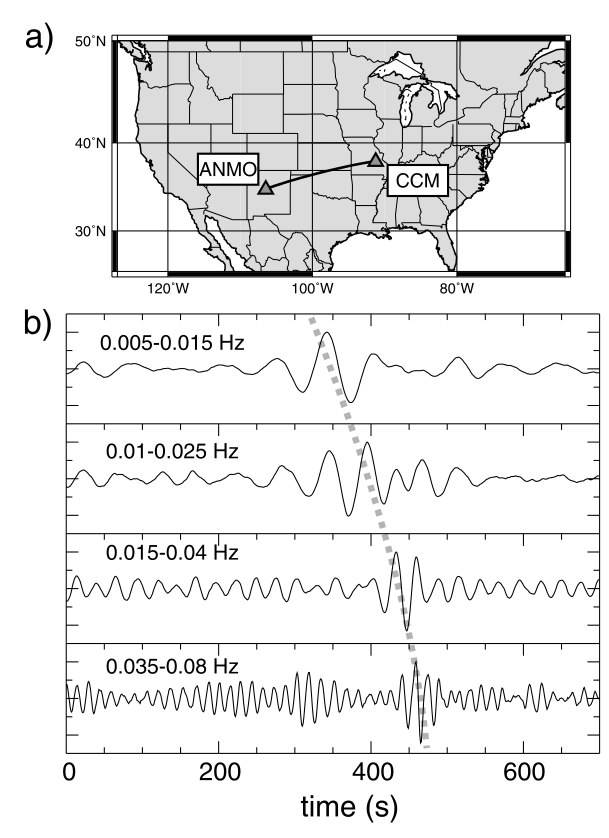
\includegraphics[scale=0.5]{Figs/shapiro2004.png}
\caption{a) Mapa mostrando a localização das estações. b) Correlações cruzadas da componente vertical dos registros com diferentes filtros de passa-banda, indicados na parte esquerda superior. Linha pontilhada dá ênfase na dispersão do sinal emergente. Extraído de \cite{shapiro_emergence_2004}.}
\label{shapiro}
\end{figure} 

\section{Processamento}

Para o processamento dos dados utilizou-se o código escrito pelo Professor Bruno Goutorbe do departamento de Geologia da Universidade Federal Fluminense. Tal código engloba: preparação dos dados, cálculo da correlação, análise Tempo/frequência e inversão tomográfica.  O código está disponível no repositório do GitHub: https://github.com/bgoutorbe/seismic-noise-tomography.

Conceitualmente o fluxo de preparação e processamento é baseado no trabalho de \cite{bensen_processing_2007}, porém algumas alterações na filtragem espectral  foram feitas devido a utilização de dados de média a alta frequência. O fluxograma \ref{fluxograma_bensen2007} representa um resumo do processamento, cada etapa mostrada no fluxograma terá uma explicação sintetizada nos tópicos a seguir.

\begin{figure}[!ht]
\centering
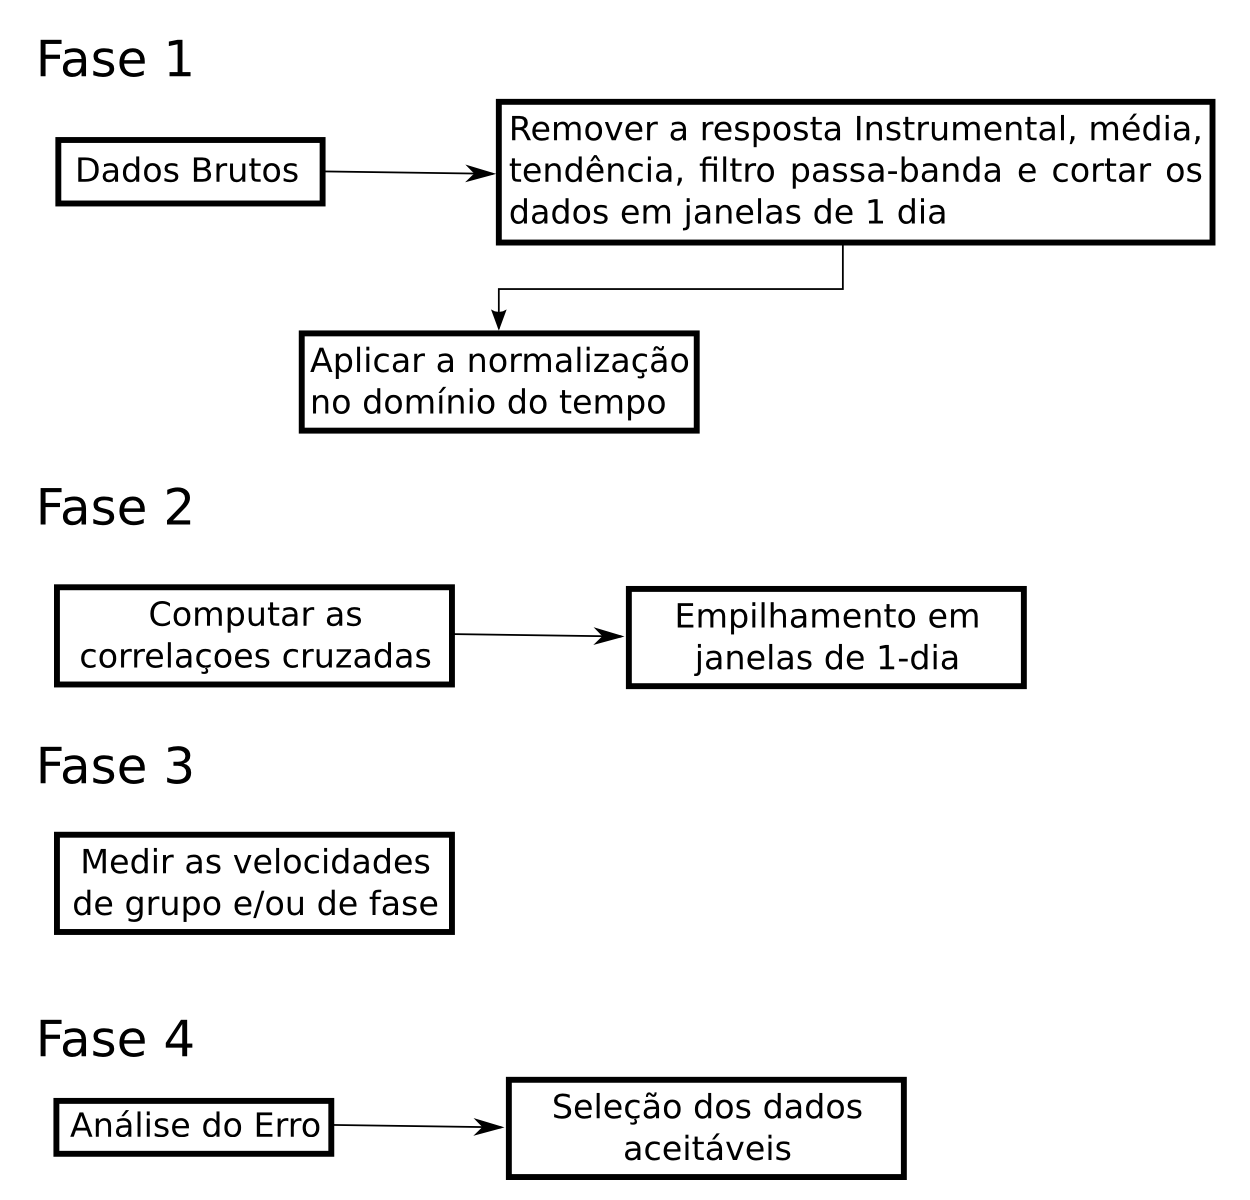
\includegraphics[scale=0.5]{Figs/fluxograma_bensen2007.png}
\caption[Representação esquemática do processamento.]{Representação esquemática do processamento. Fase 1 - etapas que involvem a preparação dos dados antes da correlação. Fase 2 - esboços do processo de correlação cruzada e empilhamento. Fase 3 -Medidas de dispersão. Fase 4 - Análise do Erro e seleção de dados aceitáveis. Adaptado de \cite{bensen_processing_2007}.}
\label{fluxograma_bensen2007}
\end{figure} 

\subsection{Preparação dos dados para cada estações}

\cite{bensen_processing_2007} cita que a primeira fase do processamento  é feita para preparar os dados da forma da onda de cada estação individualmente. Faz-se isso para acentuar o ruído ambiental de banda larga e para remover os sinais de terremoto e de irregularidades instrumentais que tendem a ocultar o ruído ambiental.

Segundo \cite{bensen_processing_2007}, séries temporáis diárias com menos que 80\% do registro devem ser rejeitadas, mas isso varia de acordo com a discretização do usuário. No caso desse trabalho foram utilizados séries  temporáis diárias com 99\% do registro, com o propósito de usar o mínimo possível a interpolação para preencher as lacunas nos registros.

\cite{bensen_processing_2007} mostra que um passo importante na preparação dos dados é a "normalização temporal" ou "normalização no domínio do tempo". Isto é feito para reduzir na correlação cruzada os efeitos de terremotos, irregularidades instrumentais e fontes de ruídos não-estacionários próximos á estação. \cite{bensen_processing_2007} compara cinco métodos diferentes para a normalização temporal, como observado na Figura \ref{temporal_norma}.

\begin{figure}[!ht]
\centering
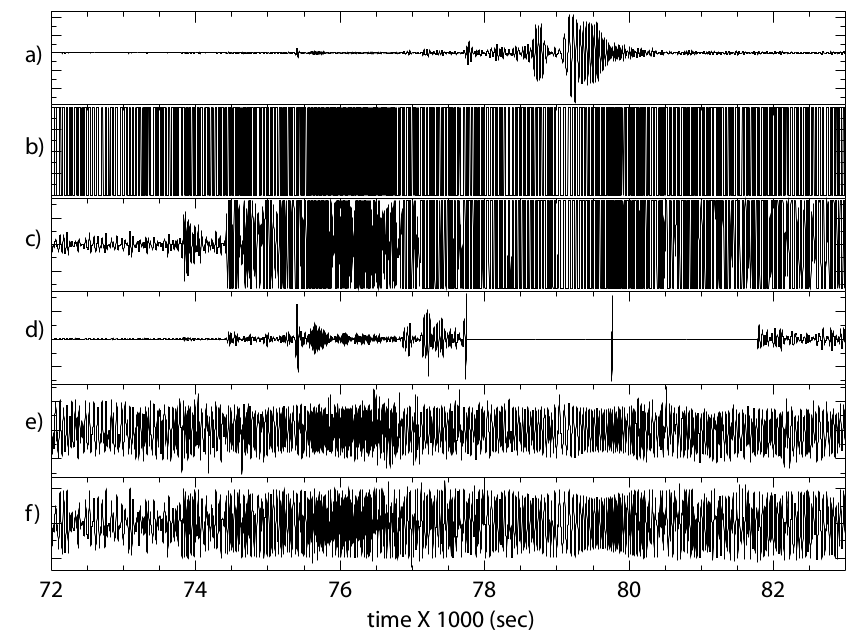
\includegraphics[scale=0.4]{Figs/temporal_norma.png}
\caption[Formas de onda mostrando exemplos de cinco tipos de normalização no dominio do tempo.]{Formas de onda mostrando exemplos de cinco tipos de normalização no dominio do tempo testadas por \cite{bensen_processing_2007}. Os exemplos estão com o filtro passa-banda entre 20 e 100 segundos e mostram a contaminação por sinais de terremoto. (a)  Dado bruto mostrando 3 horas de dados janelados em torno de um grande terremoto (M = 7.2, Afeganistão) registrado na estação ANMO. (b) Normalização 1-bit. (c) Forma de onda cortada, onde o limiar de recorte é igual ao rms da amplitude do sinal de um dado dia. (d) Evento detectado e removido automaticamente. (e) Normalização da média absoluta móvel. (f) Normalização ‘\textit{water level}’. Retirado de \cite{bensen_processing_2007}.}
\label{temporal_norma}
\end{figure} 

Terremotos geram grandes impecílios na automatização do processamento, pois eles ocorrem irregularmente e apenas grandes terremotos são encontrados nos catálogos globais, como visto na na Figura \ref{temporal_norma}-a. Então a remoção dos sinais dos terremotos tem que ser adaptativa aos dados. Muitos estudos aplicam a técnica da "normalização 1-bit", como observado na Figura \ref{temporal_norma}-b, em que somente o sinal da série temporal é retido (+1 ou -1) e a amplitude é completamente ignorada. Neste trabalho foi aplicado a "normalização da média absoluta móvel", esta produz uma razão sinal-ruído maior que a normalização 1-bit no conjunto de dados. Como mostra \cite{seats_improved_2012} em seus estudos. A "normalização da média absoluta móvel" é calculada na janela de terremotos (15 a 50 segundos) para isolar os terremotos que não são visíveis no sinal bruto.

\subsection{Normalização espectral ou braqueamento}

O ruído sísmico ambiente não é branco no domínio da frequência, ou seja, tem frequências que se destacam. \cite{bensen_processing_2007} cita que a normalização espectral atua para alargar a banda do sinal nas correlações cruzadas e atua contra a degradação causada por fontes persistentes.

A janela temporal  utilizada por \cite{bensen_processing_2007} em seu trabalho é de 7 a 150 segundos, porém quando a distância entre as estações é pequena ($\simeq 20 km$) é necessário utilizar períodos mais curtos, como é o caso desse trabalho. A banda de interesse desta dissertação é de 2 a 50 segundos, logo inclui-se o ruído de alta frequência no processamento. Com a necessidade de preservar este ruído de alta frequência, não se aplicou a normalização espectral. Testes preliminares com a normalização espectral mostraram que com a normalização espectral dos dados a qualidade em curtos perdidos era menor. 


\subsection{Correlação Cruzada, Empilhamento e  Sinal emergente}

Após preparar as séries temporais diárias, a próxima fase, como visto na Figura \ref{fluxograma_bensen2007}, é computar as correlações cruzadas e o empilhamento, mostrados na Figura \ref{correlacao_cruzada}. \cite{bensen_processing_2007} mostra que mesmo com distâncias entre as estações sendo muito longas ou curtas deve-se fazer a correlação entre todas os pares de estações possíveis. No futuro deve-se fazer a seleção das medidas aceitáveis. O número total de pares de estações possíveis é dado por $n(n-1)/2$, onde $n$ é o número de estações.

\begin{figure}[!ht]
\centering
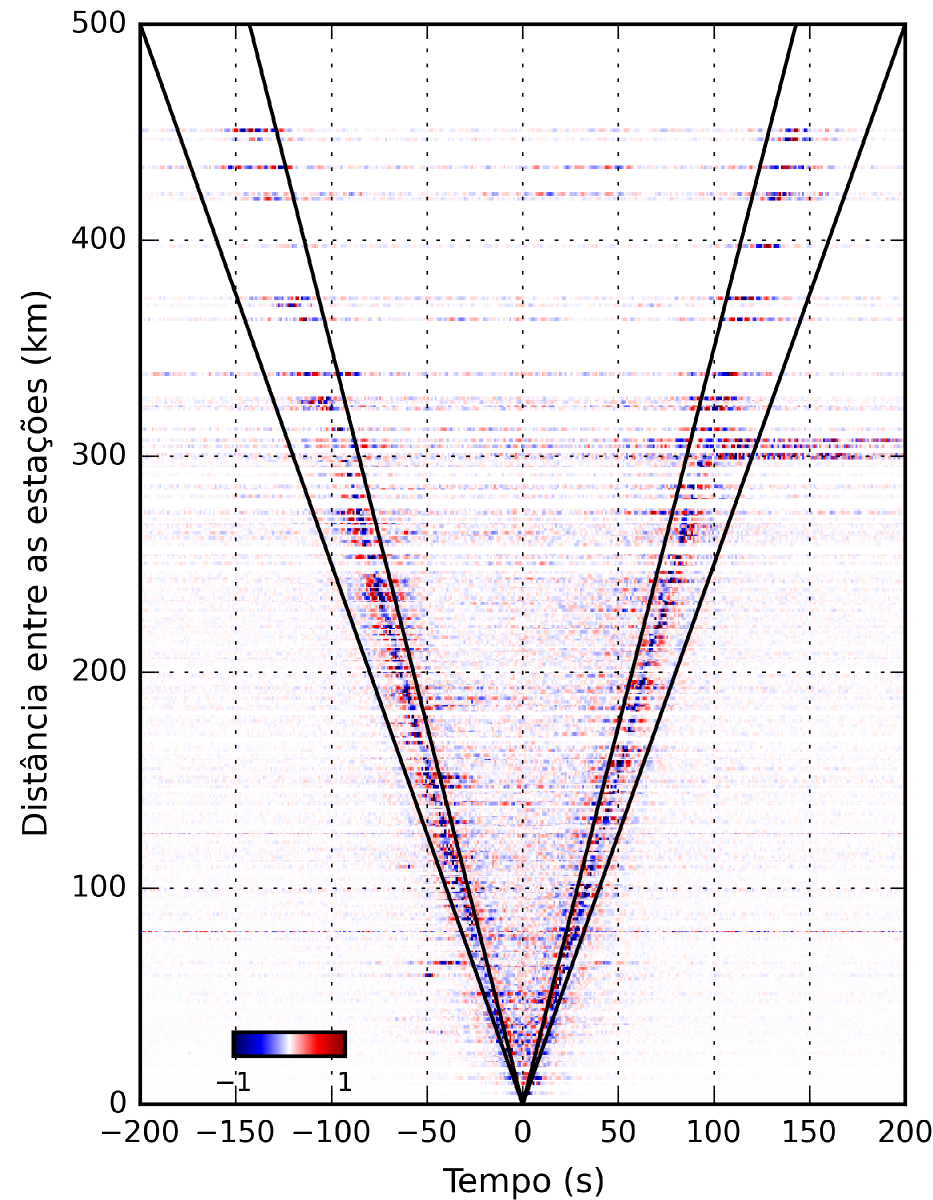
\includegraphics[scale=0.2]{Figs/correlaca_cruzada.png}
\caption[Correlações cruzadas de acordo com a distância entre as estações.]{Correlações cruzadas de acordo com a distância entre as estações. Linhas indicam as velocidades de 2.5 e 3.5 $km/s$, faixa de velocidade para as ondas de superfície. Dados foram filtrados por um filtro passa-banda entre 2 e 50 segundos.}
\label{correlacao_cruzada}
\end{figure} 

A correlação cruzada das séries temporais, com tamanho de 1 dia, é feita no domínio do tempo e empilha-se as correlações cruzadas diárias para corresponder a uma longa série temporal. 
O resultado da correlação cruzada são funções do tempo com dois lados, positivo e negativo, com coordenadas em função do tempo, isto é, correlação dos atrasos positivo e negativo, como pode ser visto na Figura \ref{correlacao_cruzada}. O tamanho da série temporal irá depender do grupo de velocidade das ondas e da distância entre as estações.

A parte positiva da correlação cruzada é chamda de sinal "causal" e a parte negativa de "acausal". \cite{bensen_processing_2007} mostra que essas formas de onda representam ondas viajando em direção opostas entre o par de estações, como mostrado na Figura \ref{correlacao_cruzada}. Se as fontes do ruído ambiental são distribuídas homegeneamente em todas as direções, a parte causal e acausal devem ser idênticas. No entanto, assimetrias consideráveis na amplitude e no espectro são observadas, indicando diferenças nas fontes e na distribuição azimutal das mesmas. \cite{bensen_processing_2007} mostra que comprimindo os dois lados do sinal, causal e acausal, em um sinal pode-se aumentar a razão sinal-ruído, o sinal resultante é chamado de sinal simétrico.

\subsection{Medidas da Dispersão}

Após o cálculo e empilhamento das correlações cruzadas diárias, a forma de onda resultante é a função de Green estimada, \cite{campillo_long-range_2003}, \cite{shapiro_emergence_2004} e, principalmente, \cite{wapenaar_retrieving_2004} e \cite{bensen_processing_2007}. Com a função de Green pode-se medir a velocidade de grupo e de fase pela análise frequência-tempo (FTAN), como mostra \cite{levshin_automated_2001}. \cite{bensen_processing_2007} diz que embora FTAN seja aplicada amplamente para fazer medidas das velocidades de grupo, curvas da velcidade de fase também são medidas naturalmente no processo.

\cite{bensen_processing_2007} exemplifica o cálculo da Dispersão das ondas no domínio da frequência por:

\begin{eqnarray}
S_{a}(\omega) = S(\omega)(1 + sgn(\omega))
\end{eqnarray}

onde $sgn(\omega)$ é a função sinal, $S(\omega)$ é a transformada de Fourier da forma de onda $s(t)$, também chamado "sinal analítico".

A transformada inversa é expressa no domínio do temppo por:

\begin{eqnarray}
S_{a}(t) = s(t) + iH(t) = \left | A(t) \right |exp(i\Phi(t))
\end{eqnarray}

onde $H(t)$ é a transformada de Hilbert de $s(t)$. Para construir a função tempo-frequência, o sinal analítico é submetido a um conjunto de filtros Gaussianos passa-banda estreitos com frequências centrais $\omega _{0}$:

\begin{eqnarray}
S_{a}(\omega,\omega _{0}) = S(\omega)(1 + sgn(\omega))G(\omega - \omega _{0})
\\
G(\omega - \omega _{0}) = e^{-\alpha(\frac{\omega - \omega _{0}}{\omega _{0}}^{2})}
\end{eqnarray}

Após a transformação inversa cada função passa-banda é retornada ao domínio do tempo produzindo uma função modulada 2-D, $\left | A(t,\omega _{0}) \right |$, e uma função da fase, $ \Phi(t,\omega _{0}) $. Onde $\alpha$ é o parâmetro que define as resoluções complementares no domínio da frequência e do tempo, \cite{levshin_automated_2001}. O tempo de chegada de grupo, $\tau (\omega _{0})$, como uma função da frequência central do filtro Gaussiano é determinado do pico da função modulada de modo que a velocidade de grupo é $U(\omega _{0})=r/\tau (\omega _{0})$, onde r é a distância entre as estações. \cite{bensen_processing_2007} substitui $\omega _{0}$ pela "frequência instantânea", como mostra \cite{bracewell_fourier_1978}. A frequência instantânea é definida como taxa de variação da fase do sinal analítico num tempo $\tau$. \cite{bensen_processing_2007} declara que esta correção é significativa quando o espectro da forma de onda apresenta picos. Devido ao vazamento espectral as frequências centrais dos filtros de bandas estreitas podem não representar fielmente o conteúdo da frequência de saída dos filtros. \cite{boashash_estimating_1992} explica detalhadamente a utilização da frequência instantânea. Para o processamento utilizou-se a frequência central para a análise tempo/frequência.

A análise frequência-tempo é descrita em duas etapas por \cite{levshin_automated_2001} e \cite{bensen_processing_2007}. A primeira etapa (FTAN bruta), filtros Gaussianos passa-banda estreitos são aplicados na representação analítica da correlação cruzada. Se o período central do filtro é $T$, o tempo em que a amplitude do sinal filtrado chega no máximo corresponde ao tempo de viagem, equivalente a velocidade de grupo $v_{g}$, da onda Rayleigh num período $T$. No entanto, deve-se garantir que a curva de dispersão, $v_{g}(T)$, é uma função suave do período, escapando de saltos causados por máximos espúrios. Isso é feito graças um algoritmo que maxima a soma das amplitudes atravessada pela curva de dispersão, e inclue um termo penalizando discontinuidades na curva.

Essa FTAN bruta é realçada com o uso de um filtro '\textit{phase-matched}', em que o termo de correção $\psi(\omega)$ é aplicado na fase dos sinal analítico no domínio da frequência. $\psi(\omega)$ é avaliado graças à curva de dispersão bruta $v_{g}(T)$ como:

\begin{eqnarray}
\psi(\omega) = \Delta \int_{\omega_{0}}^{\omega} \frac{{d\omega}'}{v_{g}({\omega}')}
\end{eqnarray}

onde $\Delta$ é a distância entre as estações e $\omega = \frac{T}{2\pi}$. Uma curva de dispersão filtrada pode então ser medida repetindo o primeiro passo com o sinal filtrado pelo termo de correção.

A variabilidade sazonal das medidas de dispersão é avaliada pelo FTAN e pelas medidas das curvas de dispersão nas correlações cruzadas obtidas dos subconjuntos sazonais trimestralmente (Jan-Fev-Mar, Fev-Mar-Abr, ... , Dec-Jan-Fev). 

\begin{figure}[!ht]
\centering
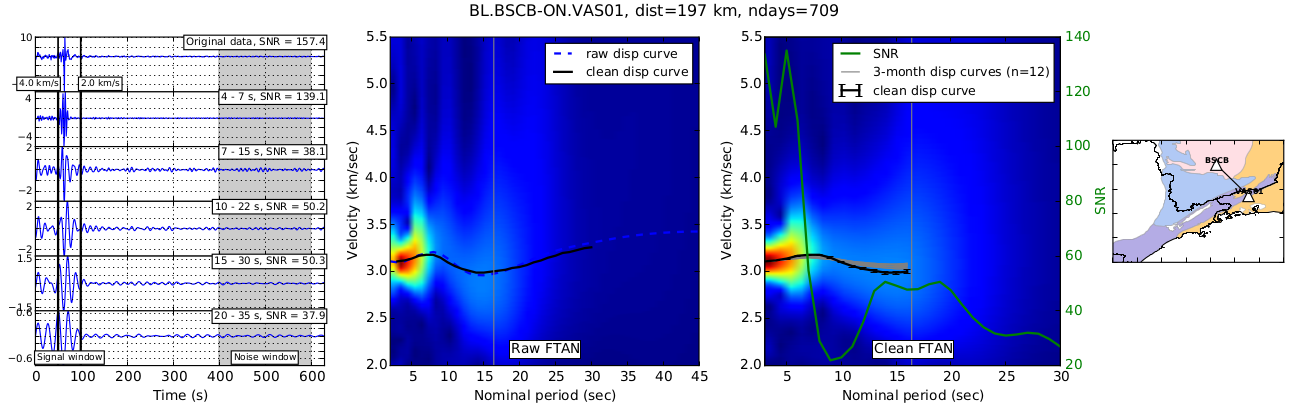
\includegraphics[scale=0.8]{Figs/correlacao_FTAN.png}
\caption[Exemplo de correlação cruzada e análise frequência-tempo (FTAN) no par de estações BL.BSCB-ON.PET01.]{Exemplo de correlação cruzada e análise frequência-tempo (FTAN) no par de estações BL.BSCB-ON.VAS01. (Esquerda) Correlação cruzada original simetrizada e filtrada com passa-banda. (Centro) Amplitude da FTAN bruta e (Direita) filtrada, normalizada por cada valor de período e curvas de dispersão das velocidades de grupo. Os dados da forma de onda foram filtradas entre 2 e 50 segundos. Mapa mostrando a localização do par de estações (estações, províncias tectônicas e divisas estaduais) na parte superior direita.}
\label{correlacao_FTAN}
\end{figure}

A Figura \ref{correlacao_FTAN} ilustra todo o processo para o par de estações BL.BSCB-ON.PET01: cálculo das correlações cruzadas, FTAN bruta, FTAN filtrada, medidas das curvas de dispersão e avaliação da variabilidade sazonal. 

\subsection{Controle de Qualidade das Medidas}

Como a quantidade de caminhos entre as estações é numerosa, o controle de qualidade das correlações cruzadas deverá ser aplicado automaticamente, assim haverá o mínimo de interação humana, logo medidas errôneas serão minimizadas. \cite{bensen_processing_2007} mostra que medidas de dispersão confiáveis devem passar pelo seguinte critério: $\Delta > 3\lambda = 3c\tau$ ou $\tau < \Delta/3c$, sendo $\tau$ o período, $c$ o comprimento de onda, $\Delta$ a distância entre as estações em quilômetros e $\lambda$ o comprimento de onda. Sendo a velocidade de fase máxima ($c$) $\sim 4 km/s$, o período máximo de trabalho é estabelecido por $\tau_{max} = \Delta/12$. \cite{bensen_processing_2007} observa uma degradação das medidas de dispersão em períodos maiores que $\tau_{max}$, como observado na Figura \ref{correlacao_FTAN}. 

Para o controle de qualidade dos dados deve-se identificar e rejeitar medidas ruins. Junto com os critérios estabelecidos por \cite{bensen_processing_2007}, anteriormente, utilizou-se a razão sinal-ruído (SNR), a razão entre o valor máximo absoluto na janela de sinal e o desvio padrão da janela de ruído. Estas janelas são estabelecidas de acordo com a distância entre as estações ($\Delta$). A janela de sinal é demarcada entre os tempos de chegada correspondentes as velocidades de 2.5 e 3.5 $km/s$, mostradas na Figura \ref{correlacao_cruzada}. A janela de ruído é demarcada 200 segundos após a janela de sinal, isso para garantir que seja apenas ruído. O SNR é calculado para cada período aplicando um filtro Gaussiano estreito centrado no período correspondente.

Outro critério estabelecido por \cite{bensen_processing_2007} é avaliar a repetibilidade temporal das medidas de dispersão. As fontes de ruído ambiental mudam sazonalmente e fornecem diferentes condições para as medições. Dadas certas condições de mudança, a repetibilidade da medição é um indicador significativo de confiabilidade. Neste procedimento calculou-se o desvio padrão para um conjunto de velocidades sazonais, estas devem ter SNR maior que 7 e no mínimo 3 dessas velocidades disponíveis. Se não for satisfeito esse critério o desvio padrão é considerado indefinido.

O conjunto de critérios para considerar as medidas de dispersão de boa qualidade para um período $T$ são:

\begin{enumerate}
\item T $\leq$ período de corte, definido no parágrafo anterior;

\item Para velocidades de grupo cujo o desvio padrão é definido: $sigma$ $\leq$ 0.1 km/s e SNR $\geq$ 7;

\item Para velociades de grupo que o desvio padrão é indefinido: SNR $\geq$ 15.
\end{enumerate}

\subsection{Inversão Tomográfica}

A metodologia desenvolvida por  \cite{barmin_fast_2001} foi utilizada para produzir os mapas de velocidade de grupo das ondas Rayleigh. Assume-se que as ondas de superfície seguem os caminhos entre os pares de estações, fazendo com que a inversão seja um problema linear em relação as vagarosidades. Logo num período ($T$) qualquer as pertubações no tempo de viagem entre os pares de estações é dada por:

\begin{equation}
d=Gm
\end{equation} 

O vetor $d$ contém o pertubações no tempo de viagem entre os pares de estações (deduzidos das velocidades de grupo medidas no período $T$), o vetor de parâmetro $m$ consite da pertubações na vagarosidade ao longo dos nós de um grade regular e a matriz sensibilidade $G$ realiza a integração entre a vagarosidade ao longo do caminho percorrido pelas ondas. As pertubações são relativas ao modelo de referência, definido como a vagarosidade média implícita por todos o tempos de propagação das ondas observados. A vagarosidade modelada é discretizada ao longo de uma grade regular de 0.1º x 0.1º. 

Introduz-se uma função de penalização que é composta por três termos:

\begin{eqnarray}
(Gm-d)^{T}C^{-1}(Gm-d) + \alpha ^{2} \left \| F(m)  \right \| ^{2} + \beta ^{2 } \left \| H(m)  \right \| ^{2}
\end{eqnarray}

O primeiro termo é o desajuste, $C$ é a matriz de covariância dos erros observacionais. $C$ é uma matriz diagonal contendo a variância dos erros nos tempos de viagens observados, deduzidos do desvio padrão das velocidade de grupo, estas velocidades são calculadas previamente. 

O segundo termo da função de penalização é a condição de suavidade espacial, que é dada por:

\begin{eqnarray}
F_{i}(m)=
 \left\{\begin{matrix}
1 \hspace{18mm} if \hspace{3mm} i = j,
\\ 
-S(r_{i},r_{j}) \hspace{3mm} if \hspace{3mm} i \neq j,
\end{matrix}\right.
\end{eqnarray}

\begin{eqnarray}
S(r_{i},r_{j}) \propto exp(- \frac{\left \| r_{i}-r_{j}  \right \|^{2}}{2\sigma ^{2}}) \\
\sum_{j\neq i} S(r_{i},r_{j}) = 1         \forall i 
\end{eqnarray}

com $r_{i}$ a posição do $i$-ésimo nó da grade e $\sigma$ a largura da suavidade espacial.

O terceiro termo penaliza a norma ponderada no modelo, isso faz com que o modelo suavize regiões onde há pouca cobertura de dados:

\begin{eqnarray}
H_{i}(m) = exp(-\lambda \rho _{i})m_{i}
\end{eqnarray}

onde $\rho _{i}$ é o número de caminhos que cruza a célula 0.1º x 0.1º centrada no $i$-ésimo nó da grade. Os parâmetros $\alpha$, $\beta$ ,$\lambda$ e $\sigma$, apresentados na Tabela \ref{tabelaPARAMETROS}, foram ajustados através de otimizações feitas por tentativa e erro.

Para identificar e remover caminhos discrepantes que podem ter passado pelo critério de seleção o procedimento passa-dois foi empregado. Inicialmente um mapa suave de velocidade é produzido através de uma inversão superamortecida. Nesta a maior parte da energia é afetada pela condição de suavidade espacial. Pares que possuem um tempo de viagem residual maior que três vezes o desvio padrão do resíduo, calculado pela diferença entre o tempo de viagem observado e predito,  são descartados. Após isso, uma segunda inversão é feita. O mapa de velocidade gerado por essa segunda inversão é o mapa de velocidade final. A porcentagem de medidas rejeitadas é menos que 2\% em todas as faixas de períodos.

\begin{savenotes}
\begin{table}[!ht]
\begin{center}
\small
\caption{Tabela com os parâmetros utilizados na inversão.}
\begin{tabular}{ l c }
\hline
{\textbf{Parâmetro}} & {\textbf{Valor}}\\
\hline
Grade de Discretização & 0.1º x 0.1º\\
$\alpha$ - Peso do termo de suavidade espacial & 3000,300 \footnote{Primeiro e segundo passo da inversão, respectivamente}
\\
$\sigma$ - Largura da suavidade espacial & 25 km\\
$\beta$ - Peso do termo de penalização da norma & 100\\
$\lambda$ - Nitidez da diminuição da função de ponderação da norma & 0.3\\
\hline
\end{tabular}
\label{tabelaPARAMETROS}
\end{center}
\end{table}
\end{savenotes}

\subsection{Análise da Resolução dos Mapas Tomográficos}

Antes de interpretar os resultados é necessário fazer uma análise da resolução dos dados, necessária para avaliar as limitações dos mapas tomográficos gerados. O processo de inversão descrito nas seções anteriores produz concomitantemente com o resultado uma matriz de resolução para cada ponto na grade. Segundo \cite{barmin_fast_2001} ajusta-se um cone para cada mapa de resolução e reporta o raio deste cone como a resolução espacial característica, isto é interpretado como a distância de separação mínima para duas anomalias para ser resolvido. A resolução não pode ser menor que duas vezes o espaçamento entre os nós. Além disso, cones que possuem os melhores ajustes de altura menores que 10\% da altura máxima são considerados ruído e são automaticamente descartados.  

As limitações dos mapas tomográficos serão avaliadas qualitativamente pelo teste de tabuleiro de damas, \textit{checkerboard}, onde os tempos de viagem observados são substituídos por dados sintéticos gerados de um modelo de anomalias  de velocidade em forma de tabuleiro de damas. O modelo tem alternado anomalias senoidais de $\pm 10\%$ em torno de um valor de velocidade padrão de 3 $km/s$. Em geral, as limitações descritas pelos tabuleiros reconstruídos são consistentes com a resolução espacial estimada.

\section{Resultados}

A análise das pertubações na propagação das ondas de superfície permitem distinguir estruturas crustais intermediárias, que por outros métodos não se tinha resolução. A resolução é controlada pela quantidade de dados e pela distância entre as estações. O foco deste trabalho são as grandes estruturas tectônicas presentes na área, como bacias sedimentares e grandes blocos crustais. A resolução deste trabalho limita-se a valores em profundidade próximos da crosta intermediária.

\subsection{correlações cruzadas}

\begin{figure}[!ht]
\centering
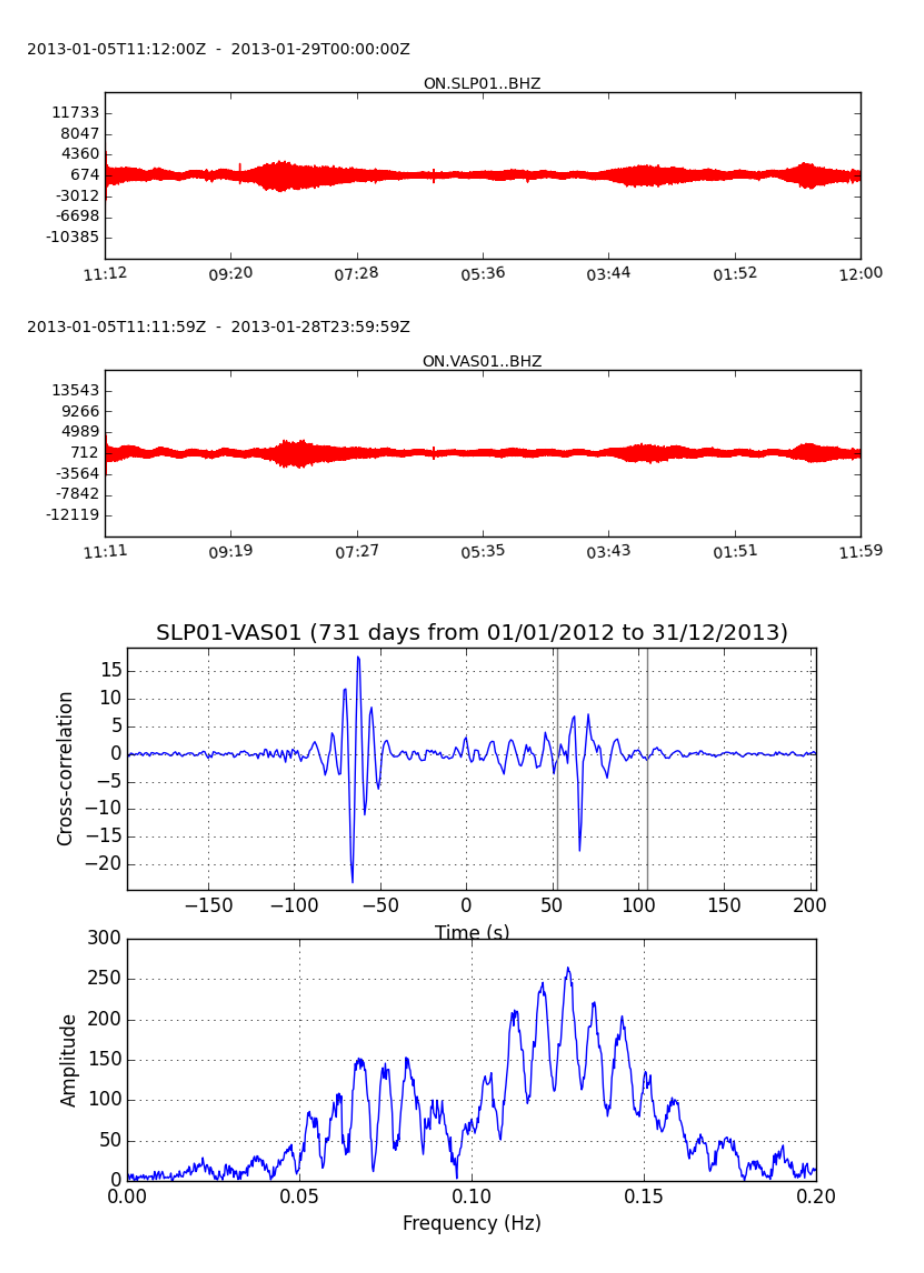
\includegraphics[scale=0.5]{Figs/corr_dado_bruto.png}
\caption[Dados Brutos das estações SLP01 e VAS01 e a correlação dos mesmos.]{Na parte superior da Figura observa-se os dados brutos do mês de Maio das estações SLP01 e VAS01 . Na parte inferior tem-se o empilhamento de 731 dias de correlações cruzadas entre as estações e o espectro deste sinal.}
\label{corr_dado_bruto}
\end{figure}

A parte superior da Figura \ref{corr_dado_bruto} mostra como é o dado após o tratamento, este dado que é processado para gerar as correlações cruzadas. A parte inferior mostra o resultado do empilhamento das correlações cruzadas diárias entre as estações SLP01 e VAS01 em 731 dias, entre os dias 01/01/2012 e 31/12/2013.  A correlação cruzada apresenta uma parte causal (positiva), esta corresponde ao deslocamento de uma onda da estação SLP01 a VAS01, e a anticausal (negativa), que representa a propagação de uma onda entre a estação VAS01 e SLP01. O sinal gerado pela correlação entre as estações SLP01 e VAS01 é assimétrico, Figura \ref{corr_dado_bruto}, assim como a maioria das correlações cruzadas geradas neste trabalho, pode ser observado na Figura \ref{correlacao_cruzada}. No caso da correlação entre SLP01 e VAS01 a maior parte da energia do sinal acumula-se na parte acausal do dado. Isso acontece devido á distribuição das fontes de ruído sísmico ambiental, pois se as fontes fossem azimutalmente bem distribuídas as correlações seriam simétricas, como mostra \cite{stehly_study_2006} em seu trabalho. \cite{stehly_study_2006} mostra a procedência das fontes de rúido sísmico ambiental e explica que as fontes possuem duas bandas espectrais, estas são separadas em primárias (10-20 segundos) e secundárias (5-10 segundos). O ruído sísmico de fundo  de alta frequência, microssismo secundário, é gerado pela interação do oceano com a costa, este tipo de fonte não sofre grandes variações por efeitos sazonais, diferentemente do microssismo primário que exibe uma variação sazonal forte. Portanto a discrepância entre as amplitudes entre as partes causal e acausal da correlação está relacionada com a posição das estações em relação ao oceano. 


\subsection{Análise tempo/frequência}

\begin{figure}[!ht]
\centering
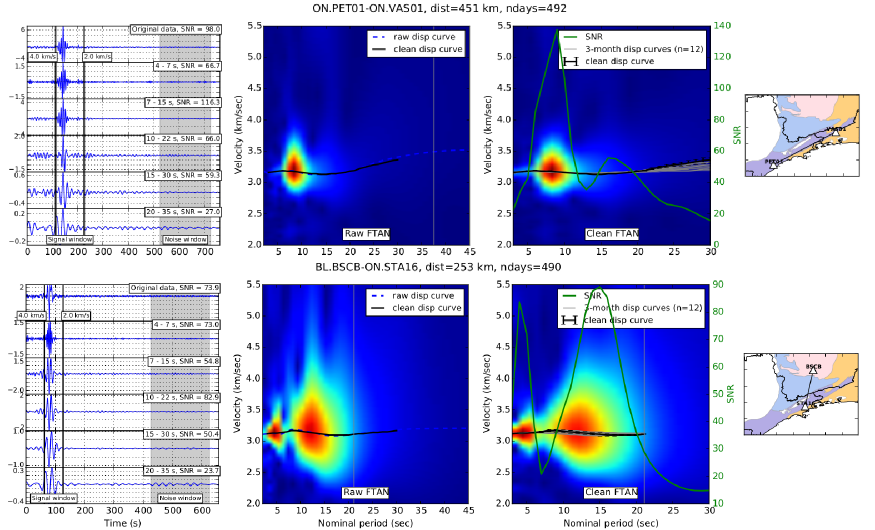
\includegraphics[scale=0.8]{Figs/fonte_FTAN.png}
\caption[Exemplos de correlação cruzada e análise tempo/frequência (FTAN) em dois pares de Estações com configurações espaciais diferentes.]{Exemplos de correlação cruzada e análise frequência tempo (FTAN) em dois pares de Estações com configurações espaciais diferentes. A parte superior mostra um par de estações com uma grande distância mostrando que a maior amplitude do sinal está no período próximo de 10 segundos. Já na parte inferior a amplitude máxima está próxima do período de 4 segundos.}
\label{fonte_FTAN}
\end{figure}

Outro ponto importante sobre as estações em relação a distância do oceano são as amplitude dos gráficos de energa gerados pela análise tempo/frequência. A Figura \ref{fonte_FTAN} e \ref{dist_FTAN} mostram exemplos de quatro pares de estações que possuem configurações distintas e geram alguns resultados interessantes sobre a pespectiva da fonte de ruído. Na Figura \ref{fonte_FTAN} observa-se que os pares em que os trajetos entre as estações estão paralelo à costa a energia contida no sinal concetra-se em volta do período de 7 segundos. Já nos trajetos que estão perpendiculares à costa há uma queda na amplitude do sinal no perído de 7 segundos. Indicando uma forte correspondência com a fonte de ruído sísmico ambiental. A relação entre a distância e a energia mostrado nas análise tempo/frequência pode ser observada na Figura \ref{dist_FTAN}. É notável que quanto maior a distância entre as estações mais informações em profundidade podem ser extraídas das velocidades de grupo. Na figura \ref{dist_FTAN} observa-se essa distribuição de energia bem marcada para ambas distâncias. Em grandes distâncias há uma  espalhamento da energia pelos períodos, porém em curtas distâncias há uma concentração de energia nos pequenos períodos. Nesta dissertação as distâncias entre as estações do projeto SUBSAL varia de $\simeq 20 km$ a $\simeq 50 km$. Portanto, o um grande número de medidas são observadas em curtos períodos com um decaimento linear bem marcado para os períodos mais longos, como pode ser observado na Figura \ref{corr_selecao}. Devido ao acentuado decréscimo do número de medidas para longos períodos, estipulou-se um período máximo para o processamento de 16 segundos, pois tem-se um número de medidas próximo de 100, considerado limite para uma tomografia de qualidade.

\begin{figure}[!ht]
\centering
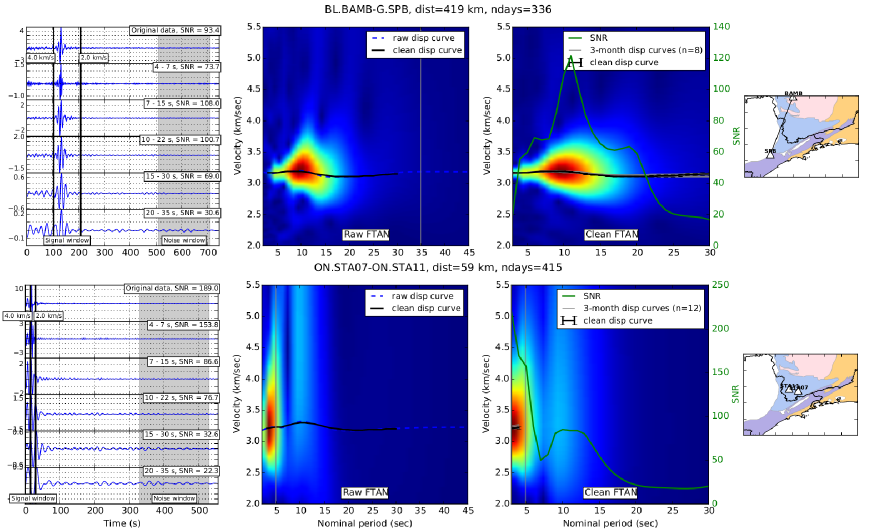
\includegraphics[scale=0.8]{Figs/dist_FTAN.png}
\caption[Exemplos de correlação cruzada e análise tempo/frequência (FTAN) em dois pares de Estações com distâncias diferentes.]{Exemplos de correlação cruzada e análise frequência tempo (FTAN) em dois pares de Estações com distâncias diferentes. A parte superior mostra um par de estações com uma grande distância mostrando que a maior amplitude do sinal está no período próximo de 10 segundos. Já na parte inferior a amplitude máxima está próxima do período de 4 segundos.}
\label{dist_FTAN}
\end{figure}

\begin{figure}[!ht]
\centering
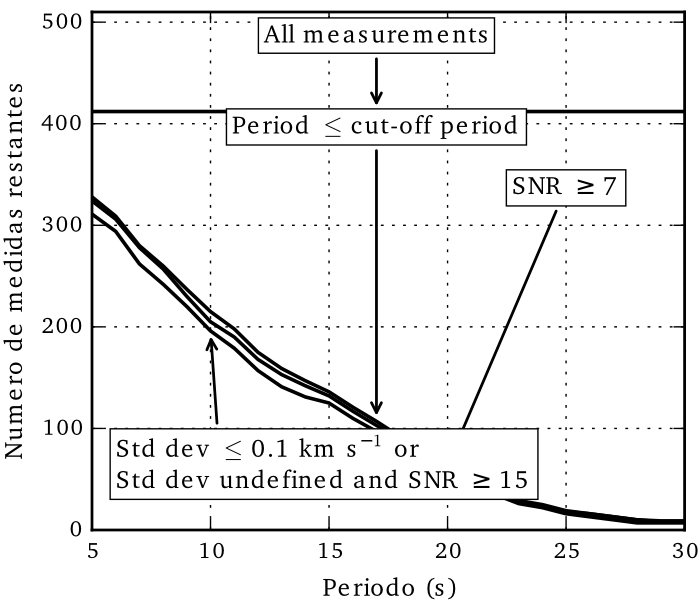
\includegraphics[scale=1]{Figs/corr_selecao.png}
\caption{Efeito do critério de seleção sucessiva na quantidade de medidas de dispersão remanescentes. Os dados de forma de onda foram filtrados entre o passa-banda 2-50 segundos.}
\label{corr_selecao}
\end{figure}

\subsection{Controle de qualidade}

Para analisar qualitativamente as correlações cruzadas utilizadas na tomografia sísmica, comparou-se a razão sinal-ruído em cada período, o resultado pode ser visto na Figura \ref{SNR}. A razão sinal-ruído é calculada pela diferença de amplitude entre a janela de sinal e a janela de ruído. È visível que em curtos períodos as correlações cruzadas possuem um sinal ruído maior, e que há um decrescimento da razão sinal-ruído com o aumento do período. Com isso a resolução em curtos períodos é maior que em longos períodos,

\begin{figure}[!ht]
\centering
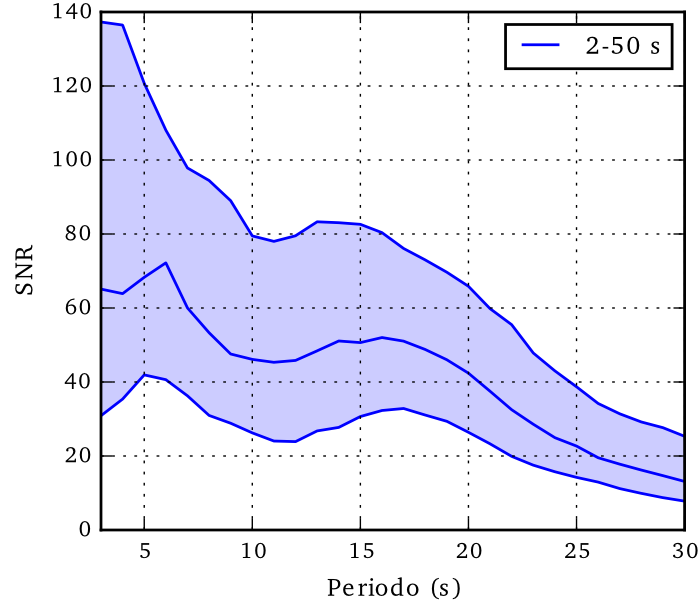
\includegraphics[scale=1]{Figs/SNR.png}
\caption{25\%,50\% e 75\% do  SRN total das correlações cruzadas em função do período. As correlações cruzadas são calculadas com um filtro passa-banda entre 2 e 50 segundos.}
\label{SNR}
\end{figure}

\subsection{Tomografia Sísmica}

A grande quantidade de trabalhos, puramente geológicos ou geológico-geofísicos, produziu uma extensa bibliografia sobre a área, porém não delimitou as estruturas crustais com um certo grau de detalhe. Com a tomografia sísmica tenta-se recuperar essas grandes feições, e para tal testou-se a sensibilidade das velocidades  de grupo das ondas Rayleigh para os seguintes períodos 5, 10 e 16 segundos, Figura \ref{sensibilidade}. Essas sensibilidade foram calculadas para um modelo com essa configuração estrutural: crosta superior de 20 km e crosta inferior de 15 km. Com as sensibilidades calculadas pode-se delimitar a profundidad de atuação de cada período, para este modelo. O período de 5 segundos tem uma sensibilidade de 4 quilômetros, já o modelo de 10 segundos 7 quilômetros e o de 16 segundos de 13 quilômetros, como observado na Figura \ref{sensibilidade}.

\begin{figure}[!ht]
\centering
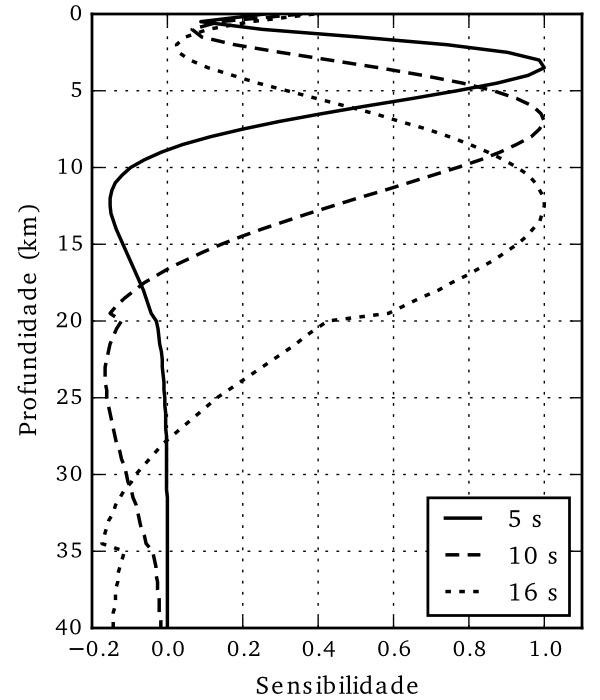
\includegraphics[scale=1]{Figs/sensibilidade.png}
\caption[Sensibilidade das velocidades de grupo das ondas Rayleigh num período selecionado]{Sensibilidade das velocidades de grupo das ondas Rayleigh num período selecionado, normalizada para a unidade. Sensibilidade é definida como a variação na velocidade de grupo causada por uma pequena variação em $V_{s}$ em uma dada profundidade. Essas sensibilidades foram calculadas para um modelo de crosta com uma crosta superior de $20$ km e uma crosta inferior de $15$ km sobre um manto.}
\label{sensibilidade}
\end{figure}

Analisando os mapas de velocidade gerados pela inversão tomográfica, Figura \ref{tomografia}-esquerda, observa-se que as grandes feições estruturais da região foram bem delimitadas nos mapas, como a Bacia do Paraná, Bacia de Taubaté, Faixa Brasília, principalmente no mapa com período de 5 segundos. Os resultados foram descritos tendo como base as unidades tectônicas regionais.

A Bacia do Paraná é a uma grande estrutura regional bem delimitada por todas os mapas tomográficos. O mapa com 5 segundos de período delimita claramente a bacia apresentando uma grande anomalia de baixa velocidade. Porém quanto nos períodos mais longos, 10 e 16, a anomalia de baixa velocidade não é bem delimitada, provavelmente devido a baixa resolução espacial. 

A Bacia de Taubaté também é uma estrutura que possui uma anomalia negativa de velocidade marcante. Mesmo sendo uma bacia pouco profunda é representada nos períodos de 5 e 10 segundos. Já no período de 16 segundos não existe nenhuem indício.

A Faixa Brasília apresenta uma anomalia positiva no período de 5 segundos, porém no período de 10 segundos essa anomalia se torna negativa e no período de 16 segundos volta a ser positiva. Essa mudança de velocidade é um resultado concordante com modelos geofísicos da região, como \cite{sand_franca_crustal_2004}, \cite{flora_solon_ancient_2013} e \cite{Silva_2014}, pois essa mudança estaria relacionada com uma inversão de velocidade devido a Zona de interferência com a Faixa Ribeira. Na parte geológica \cite{trouw_new_2013} mostra a evolução da zona de superposição em que rochas supracrustais são soerguidas gerando o sistema de \textit{Nappes}, mostrado no perfil \ref{perfil_esquematico}, explicando assim essa anomalia de baixa velocidade.

O Cráton do São Franciso possui uma anomalia de velocidade positiva nos mapas de período 5 e 10 segundos, o que era de se esperar de uma área cratônica, porém no mapa de 16 segundos apresenta uma anomalia de velocidade negativa. Tal anomalia encontra-se na Zona de interferência do Cráton com a Faixa Ribeira. \cite{heilbron_serra_2013} mostra que há uma uma imbricação de domínios tectônicos na borda sudeste do Cráton do São Francisco. Nesta amalgamação terrenos metassedimentares Neoproterozóicos, outrora bacias sedimentares, pode ter sidos carreados para grandes profundidades, pois existem sedimentos de arcos magmáticos associados a essa região \citep{heilbron_evolution_2010}, \citep{heilbron_serra_2013} e \citep{trouw_new_2013}. 

A Faixa Ribeira apresenta resultados bem parecidos nos períodos de 5 e 10 segundos, anomalias positivas de velocidade associadas aos arcos Rio Negro, a sudeste, e Socorro, a sudoeste. Uma anomalia negativa de velocidade associada a Bacia de Taubaté e a região costeira próxima ao litoral sul de São Paulo, podendo ter influência de bacias sedimentares costeiras. Uma característica interessante é a anomalia de baixa velocidade na região sudoeste da Faixa Brasília no mapa de 16 segundos, porém não foi encontrado na literatura algo que faça referência a essa anomalia de baixa velocidade. Essas anomalias negativas devem ser tratadas com cuidado, pois estão localizadas nos limites dos mapas tomográficos e assosciadas somente a uma estação. 

\begin{figure}[!ht]
\centering
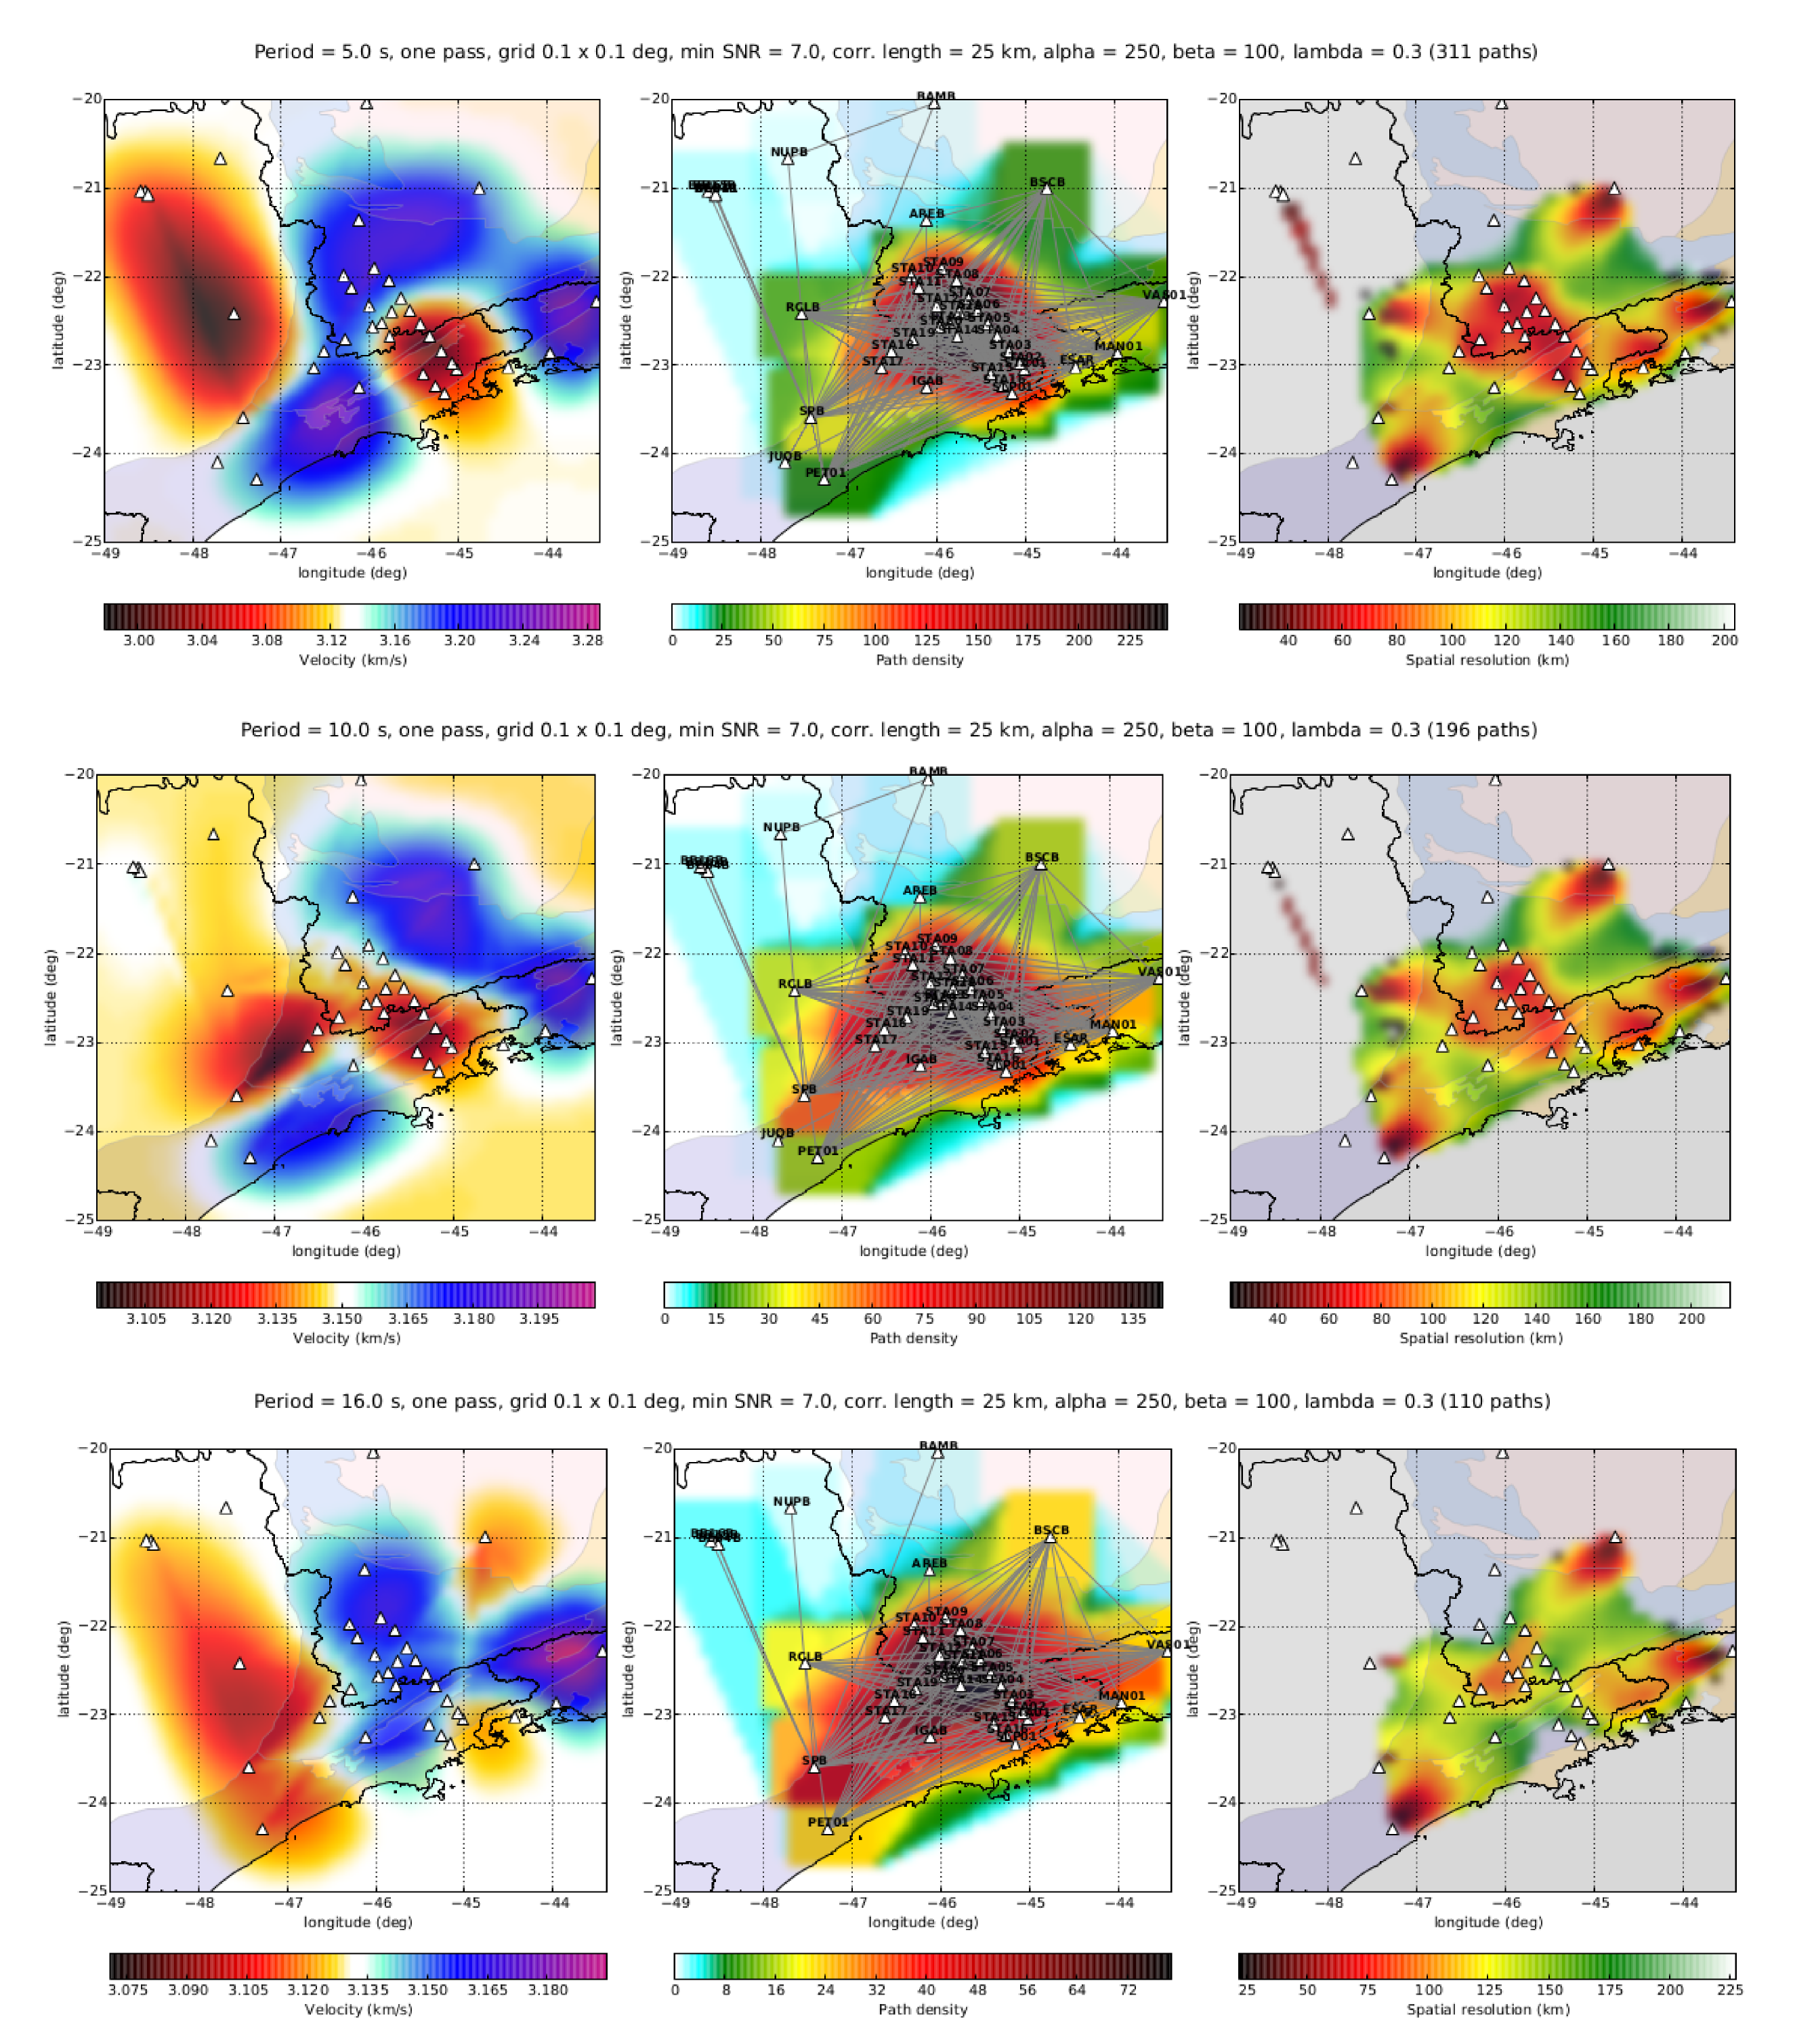
\includegraphics[scale=0.45]{Figs/mapa_tomografia.png}
\caption[Mosaico contendo as pertubações nas velocidades de grupo, trajetórias entre as estações e a resolução espacial.]{Esquerda: Pertubações nas velocidades de grupo nas ondas Rayleigh relativas a velocidade média sobre o mapa no períodos de 5, 10 e 16 segundos. Centro: Trajetórias entre as estações válidas para a inversão tomográfica. Direita: Resolução espacial definida como o raio do cone que melhor ajusta o mapa de resolução em cada ponto. Ao fundo encontra-se o mapa geológico da regional.}
\label{tomografia}
\end{figure}

As colunas central e direita da Figura \ref{tomografia} mostram a densidade de trajetórias e a resolução espacial para a tomografia sísmica. Os resultados tiveram como base a resolução espacial da tomografia. Nota-se claramente que com o aumento do período há uma diminuição da resolução espacial devido a redução do número de caminhos. A região que possui a melhor resolução espacial é a região em que se localiza a rede SUBSAL.

\pagebreak

\chapter{Resultados e Discussões}

Pesquisas envolvendo a propagação de ondas sísmicas no interior da Terra auxiliam na determinação da estrutura da mesma. Essas análises permitem recuperar, de acordo com a resolução, a geometria das descontinuidades de propriedades físicas terrestres, principalmente a velocidade de propagação das ondas de corpo.  

O método da Função do Receptor, desenvolvido por \cite{Langston_1977}, gera informações sobre a estrutura abaixo da estação sismográfica. A confiança nos resultados gerados pelo método varia em função da quantidade e qualidade das Funções do Receptor. Por isso é importante que a estação esteja funcionando corretamente e tenha uma grande quantidade de dados disponíveis.

Será dado enfoque as fases de função do receptor relacionadas à discontinuidade de Moho, interface Crosta-Manto, e reflexões  internas, antes de 5 segundos. Os resultados obtidos pelas estações temporárias serão comparados com a estação SLP01, estação permanente próxima a região de estudo, como mostrado na Figura \ref{RF_SLP01_STA08}. Assim aumentando a confiabilidade nos dados gerados pela rede de estações temporárias.

A Figura \ref{RF_SLP01_STA08} mostra as Funções do Receptor obtidas a partir de vários eventos na para a estação permanente SLP01 e para a estação temporária STA08, estas funções organizadas de acordo com o backazimute. Estes sinais estão normalizados pela amplitude do primeiro pico. O primeiro pick é a chegada da onda P direta, já o segundos, por volta de 5 segundos, e a onda P convertida em onda S na discontinuidade de Moho. As linhas verticais pontilhadas demarcam os tempos teóricos de chegada para cada múltipla. As multiplas $PpPs$ e $PpSs+PsPs$ tem uma amplitude menor que a onda P convertida em S($Ps$) devido a grande distância entre o ponto incidente e a estação. Então entas reverberações são mais afetadas por variações laterias, espallhamento e atenuação inelástica. Os sismosgramas não apresentam clareza quanto a essas reverberações. A múltipla $PpPs$ não é observada facilmente e a múltipla $PpSs+PsPs$ está mascarada pelo ruído.

\begin{figure}[!ht]
\centering
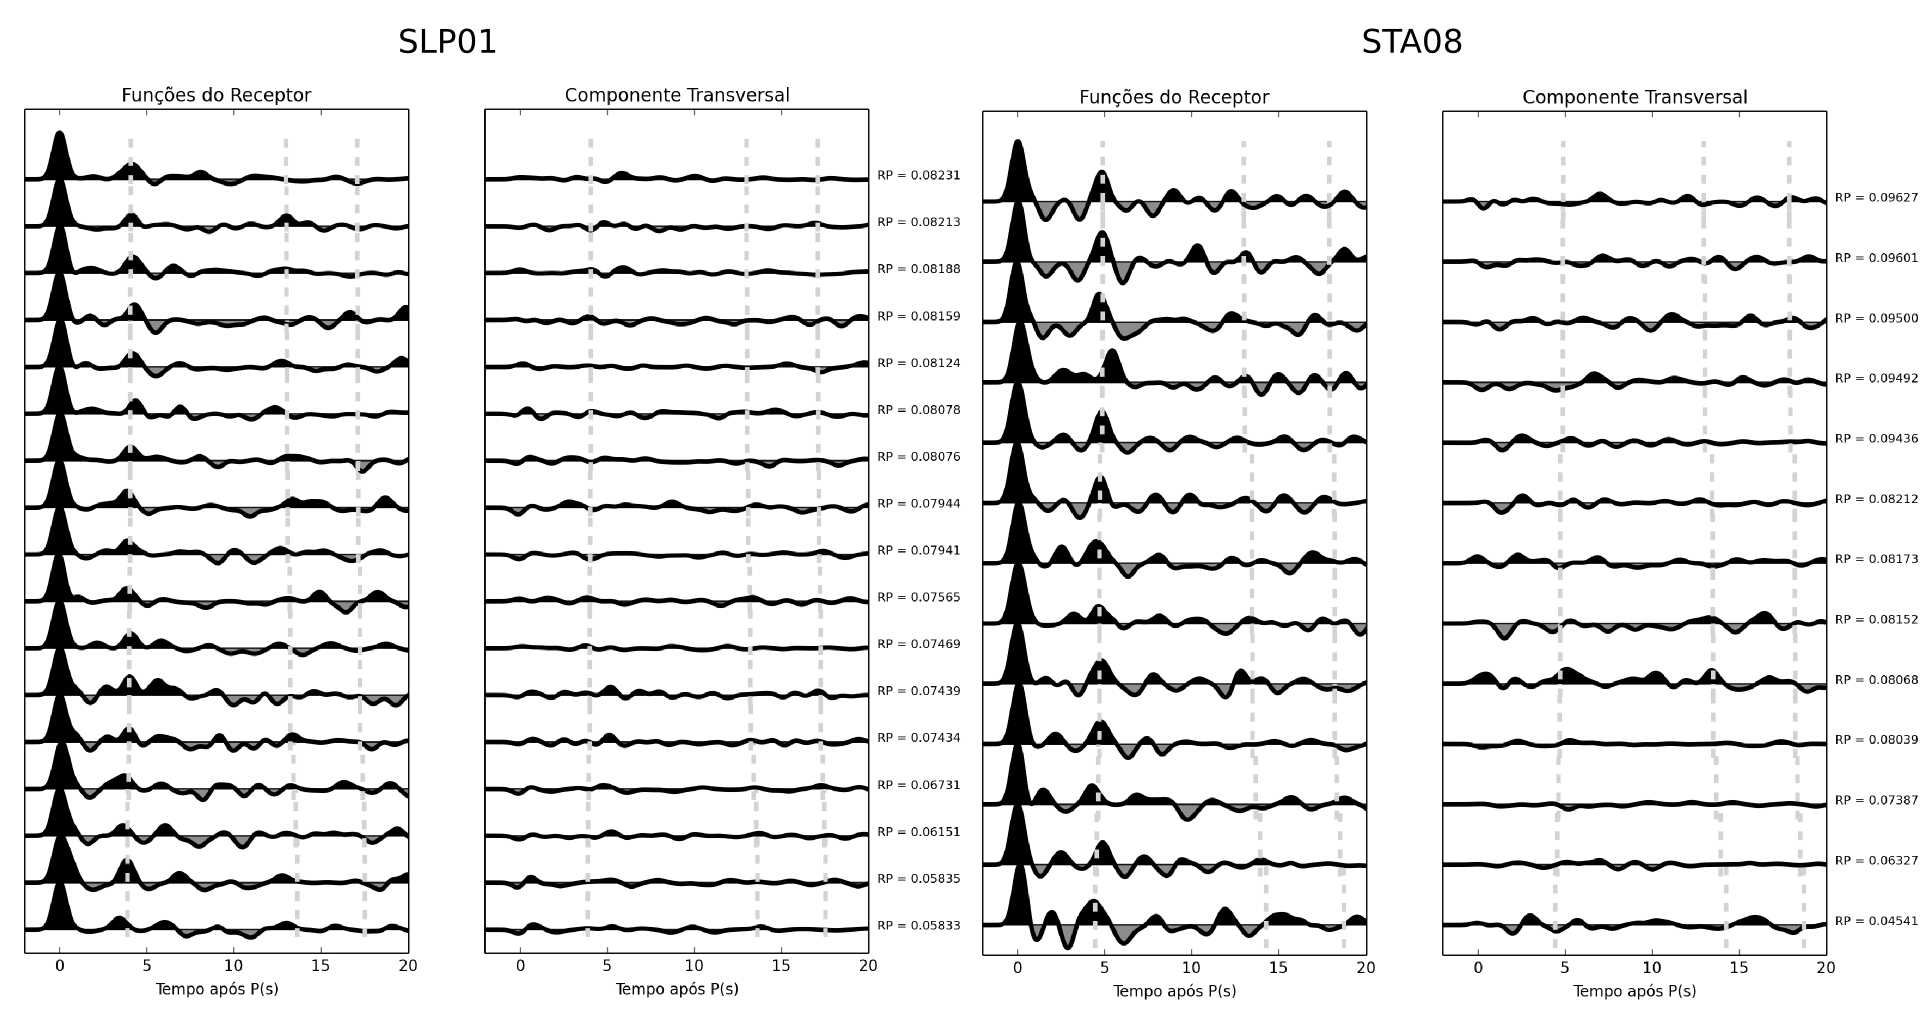
\includegraphics[scale=0.16]{Figs/RF_SLP01_STA08.png}
\caption[Exemplos de Funções do Receptor e da Componente Transversal para as estações SLP01(permanete) e STA08(temporária) distribuídas em função do parâmetro do Raio.]{Exemplos de Funções do Receptor e da Componente Transversal para as estações SLP01(permanete) e STA08(temporária) distribuídas em função do parâmetro do Raio. O primeiro pico significa a chegada da onda $P$ direta. Já o segundo a conversão da onda $P$ em $S$ em Moho. As outras múltiplas geradas em Moho não são observáveis. A linha pontilhada simboliza os tempos de chegada teóricos calculados segundo o modelo de \cite{kennet_iaspei_1991}.}
\label{RF_SLP01_STA08}
\end{figure}

DISCUSSÕES SOBRE A COMPONENTE TANGENCIAL - SAVAGE(1998)

Com as Funções do Receptor calculadas, utilizou-se a método desenvolvido por \cite{Zhu_Kanamori_2000} para calcular a profundidade de Moho e a razão $v_{p}/v_{s}$ nas estações sismográficas. Os resultados gerados estão descritos na tabela \ref{tabela1}. Para uma melhor visualização dos resultados gerados, as profundidades de Moho foram interpoladas. Para melhorar a distribuição espacial das profundidades de Moho adicionou-se dados de \cite{Assumpcao_Brazil_2013}. O mapa da interpolação pode ser visto na Figura \ref{Interpolacao}. Nota-se na Figura \ref{Interpolacao} que a discontinuidade de Moho estimada é maior no interior do continente do que na região costeira, corroborando com os dados de \cite{Assumpcao_America_2013}, \citep{Assumpcao_Brazil_2013} e \cite{van_der_meijde_gravity_2013} . 

\begin{figure}[!ht]
\centering
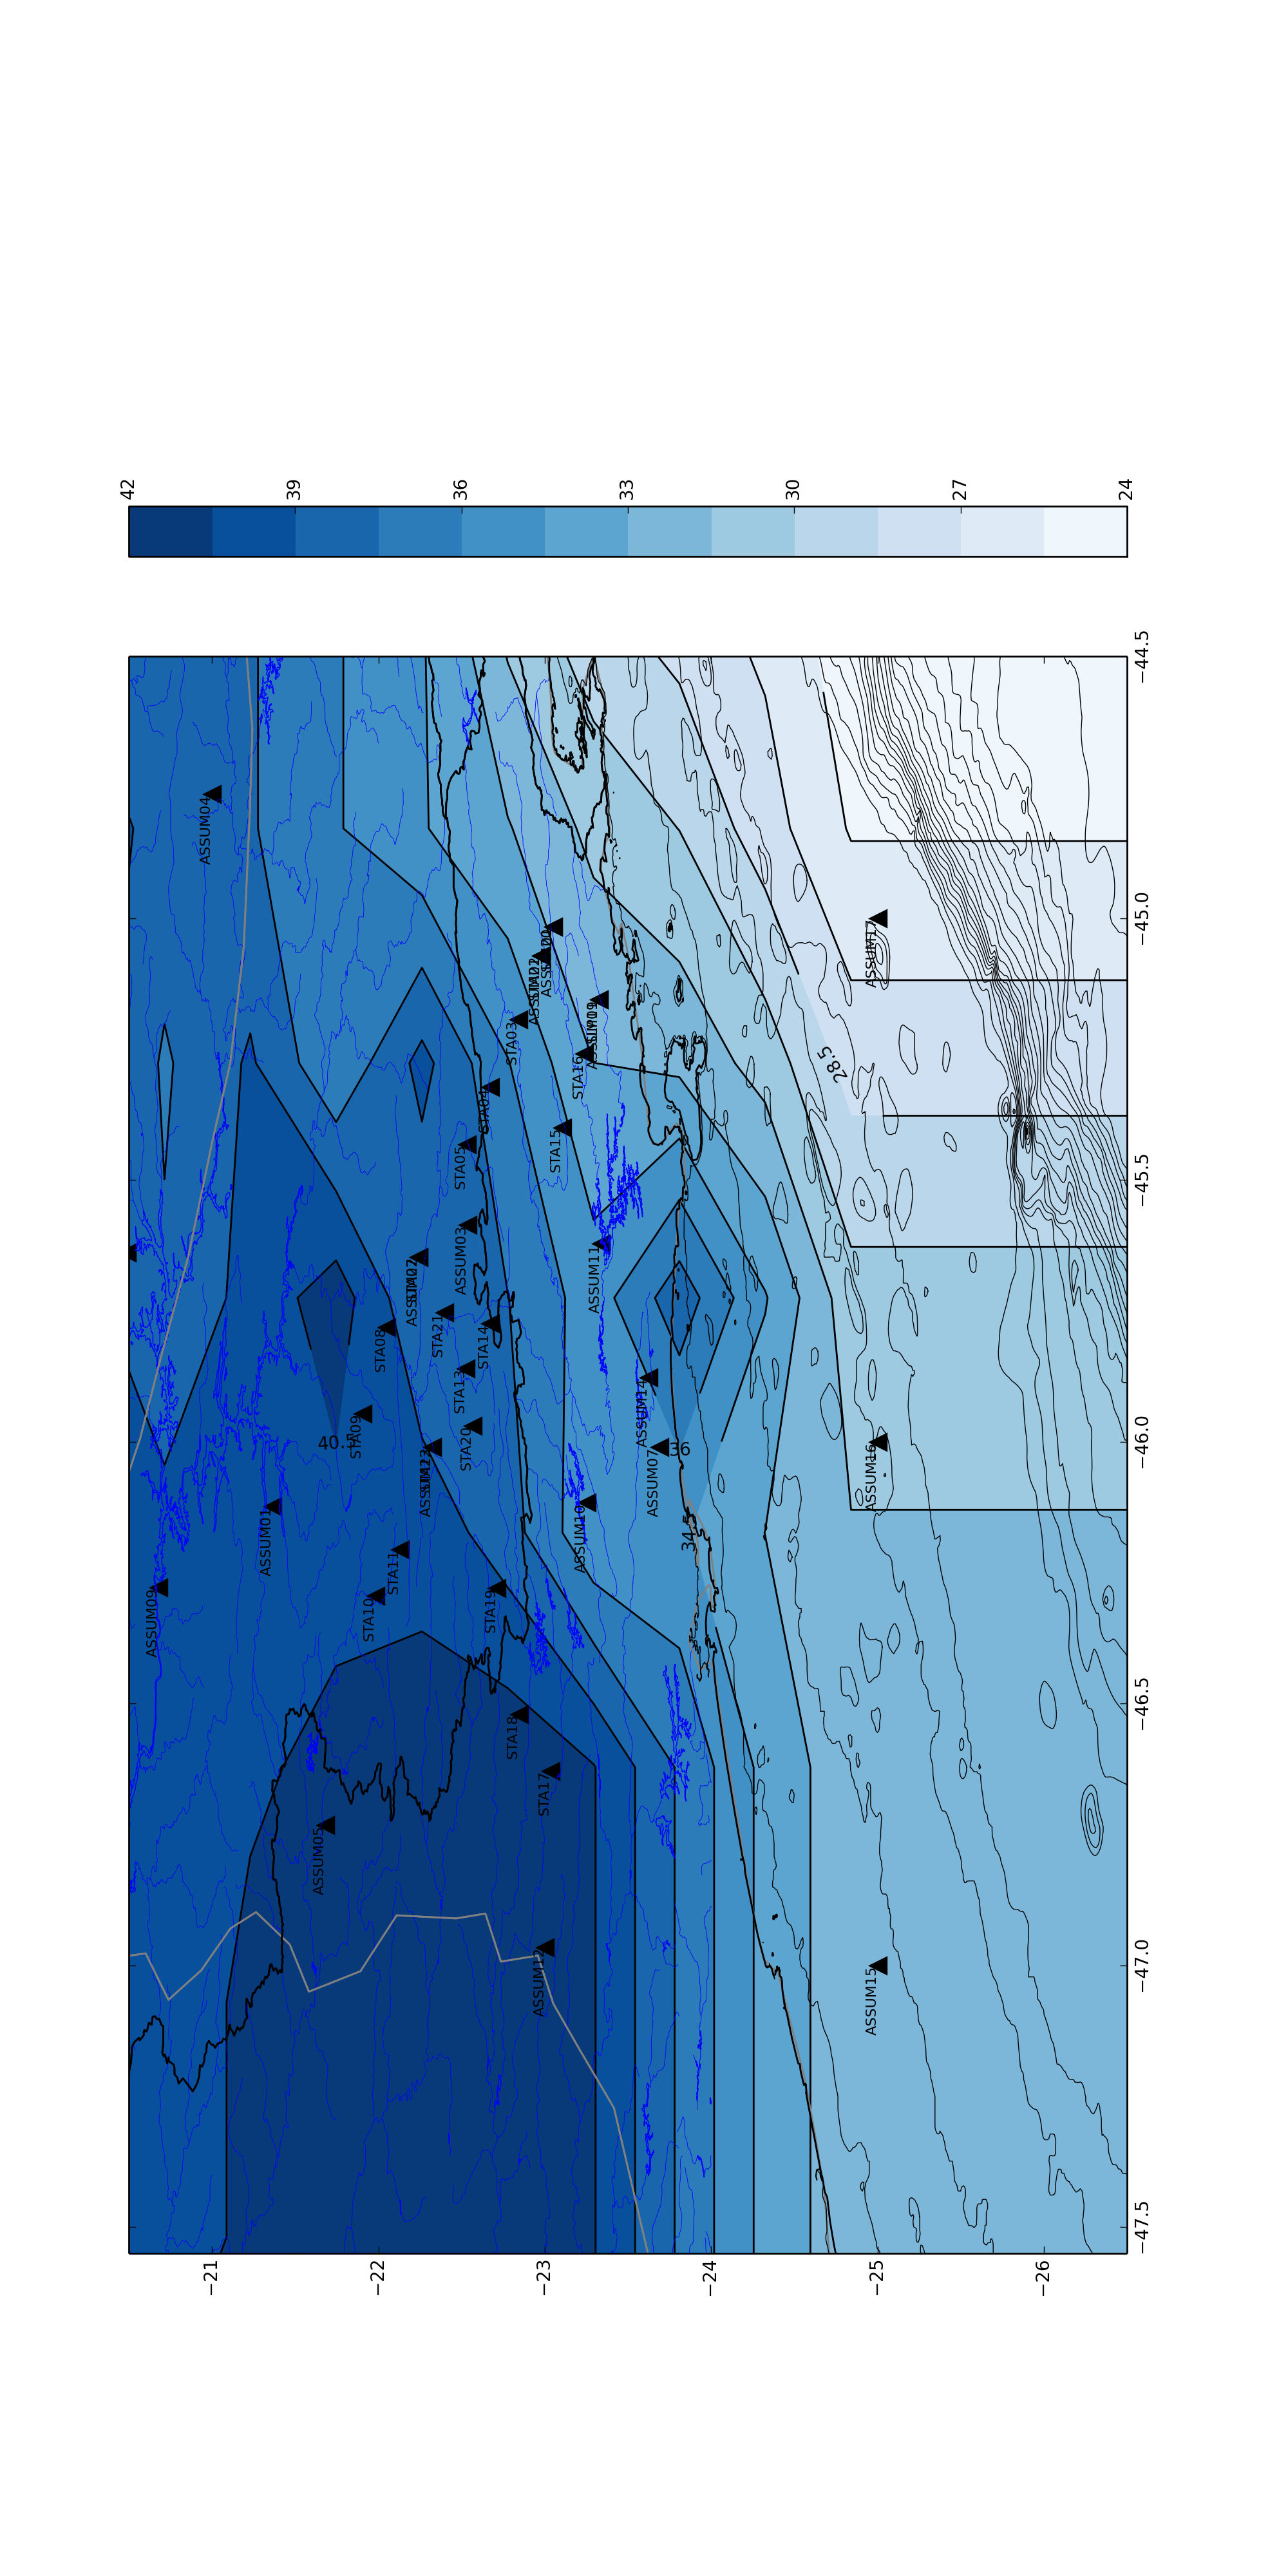
\includegraphics[scale=0.20]{Figs/Interpolacao_Linear.png}
\caption{Mapa da espessura crustal da Faixa Ribeira. Os triângulos representam as estações sismograficas.}
\label{Interpolacao}
\end{figure}

As incertezas na medidas, mostradas na Tabela \ref{tabela1}, estão diretamente ligadas a quantidade e qualidade das Funções do Receptor. A seleção das melhores Funções do Receptor é um fase importante, pois a qualidade da Função do Receptor é prepoderante sobre a quantidade. A imprecisão associada a cada um dos parâmetros obtidos pelo método de \cite{Zhu_Kanamori_2000} é estimada pelo método "\textit{bootstrap}", desenvolvido por \cite{efron_statistical_1991}. Neste trabalho utilizou 200  subconjuntos para se fazer a estimativa das incertezas associadas ao  cálculo da profunidade de Moho e da razão $v_{p}/v_{s}$.

\begin{figure}[!ht]
\centering
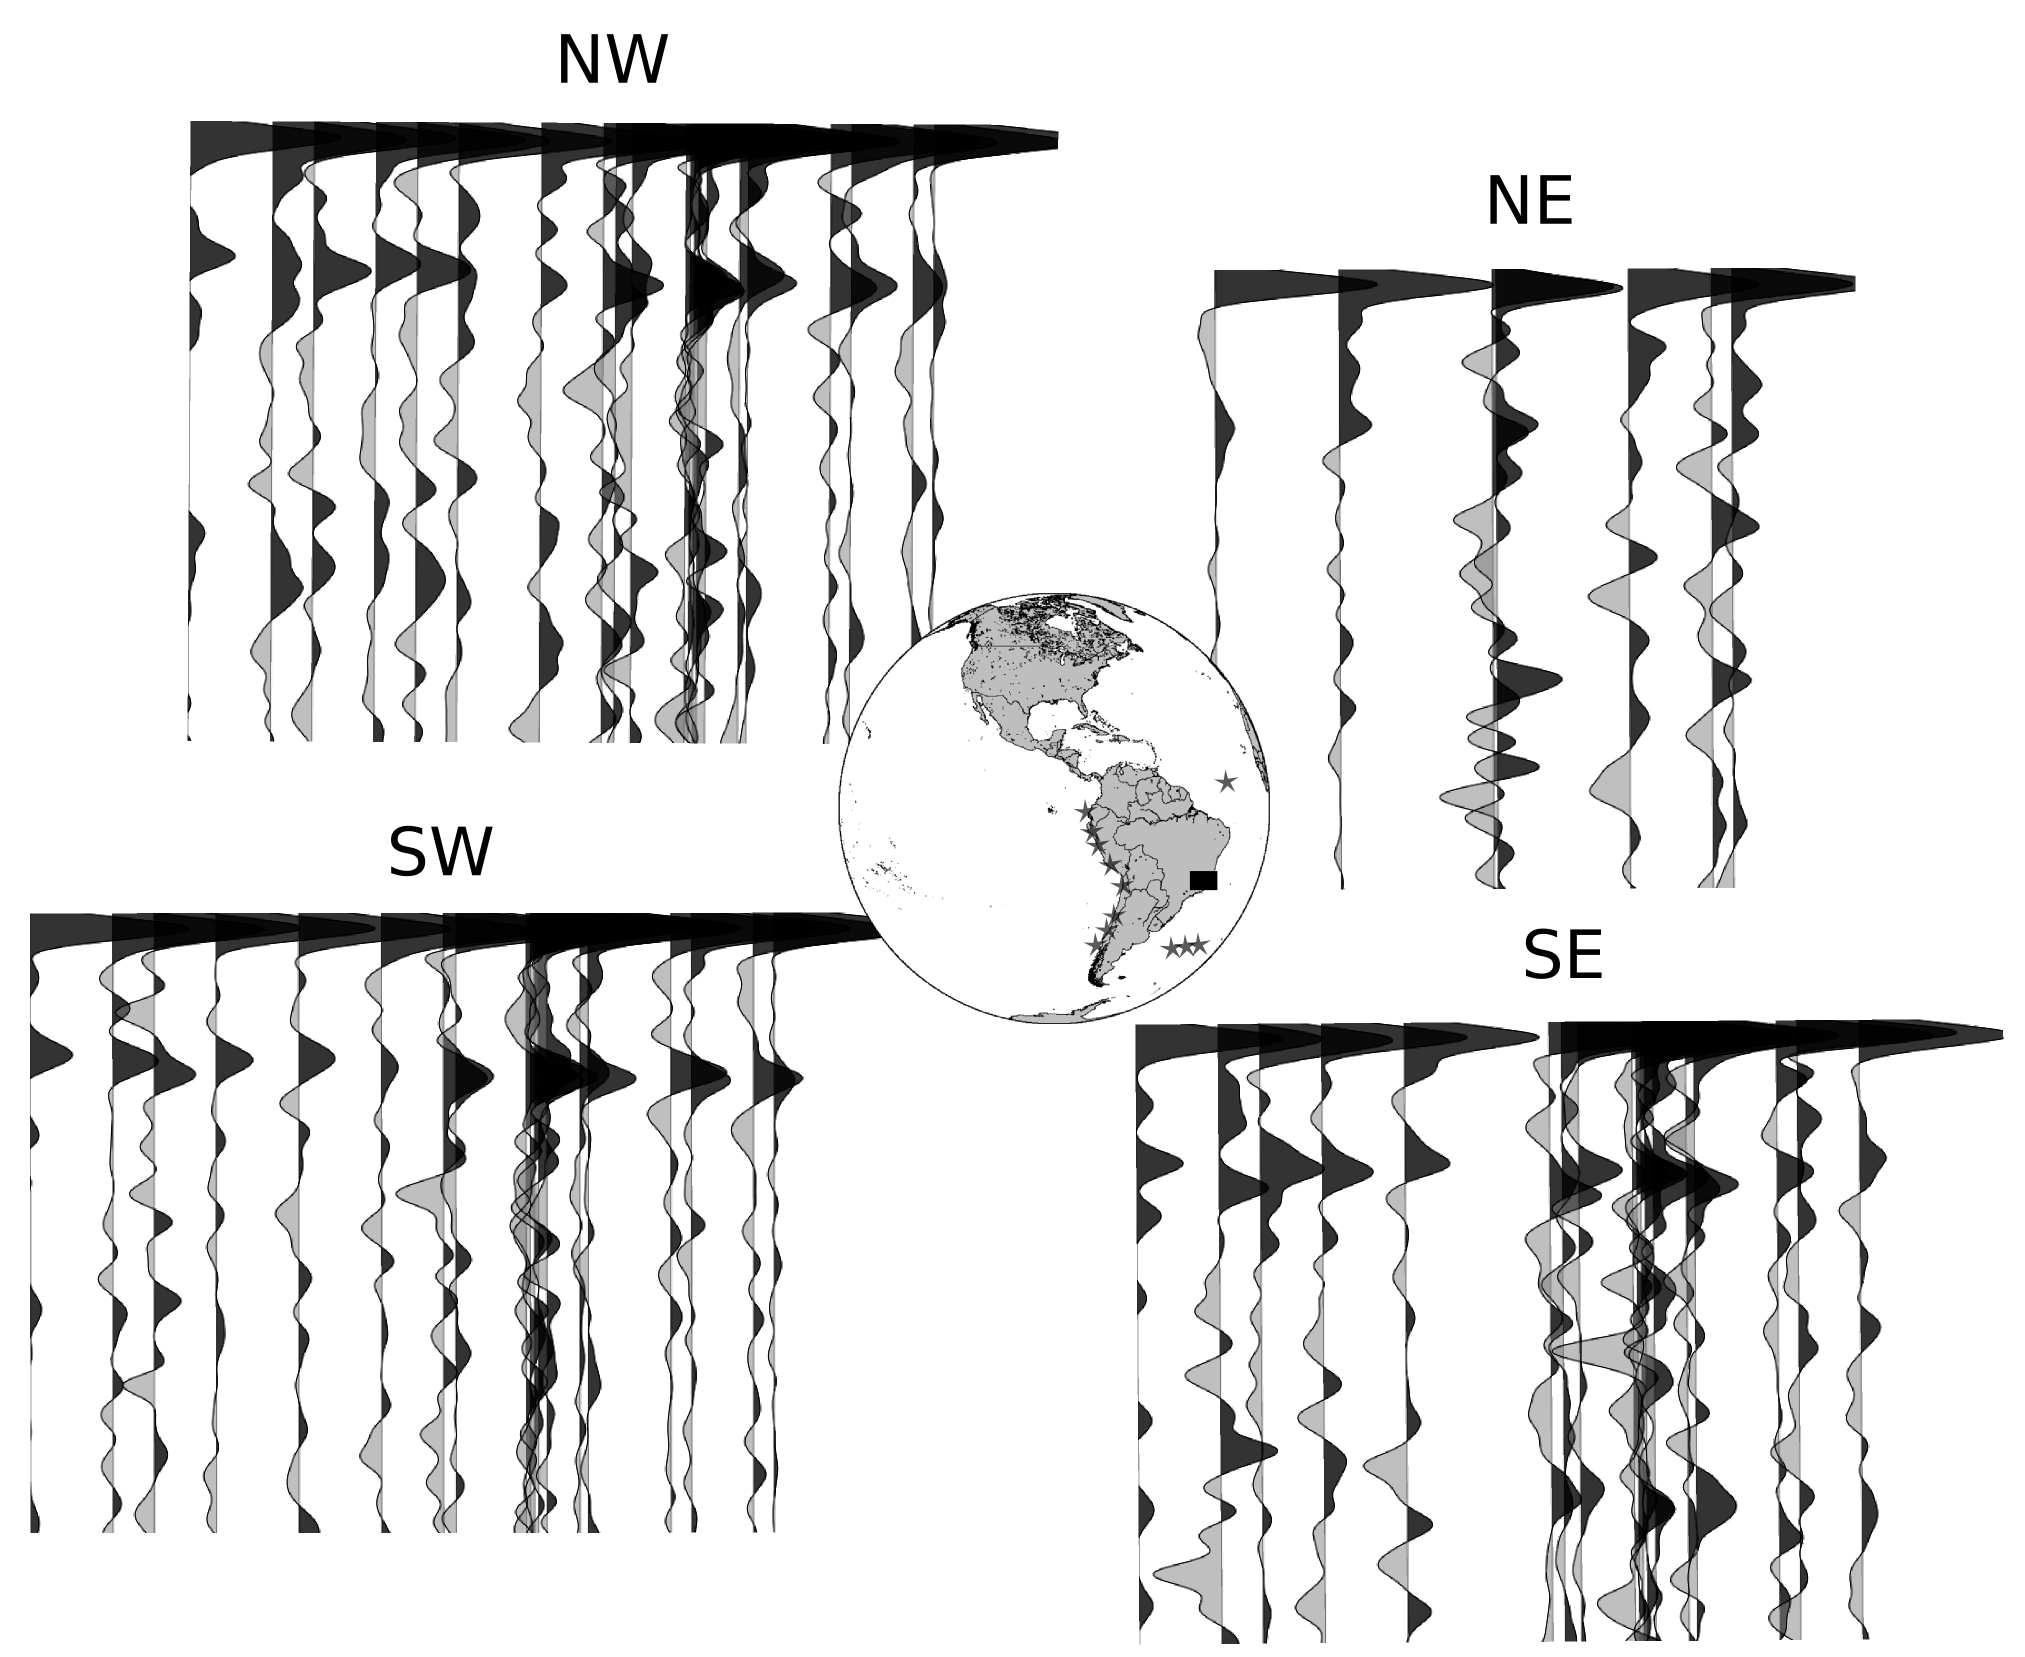
\includegraphics[scale=0.5]{Figs/RF_azimute.png}
\caption{}
\label{RF_perfil_NW}
\end{figure}


%Identfica-se sinais precursores a Moho, por volta de 2 a 4 segundos, que variam ao longo do perfil. Estes sinais podem ser relacionados com uma interface com um alto contraste de propriedade fisica. O pulso negativo antes de 5 segundos indica, segundo as modelagens propostas na Figura \ref{modelagem}, uma camada com baixa velocidade.

\chapter*{Conclusões}	
%\addcontentsline{toc}{chapter}{Referências Bibliográficas}
\bibliographystyle{seg}  
\bibliography{tese_ref}
\chapter*{Anexo 1}	


\begin{center}
\begin{table}[!ht]
\caption{Tabela com as coordenadas(Lat Long) e altitude (m) das Estações.}
\begin{center}
\begin{tabular}{| c | c | c | c |}
\toprule
{\large \textbf{Nome}} &	{\large \textbf{Latitude}} & {\large \textbf{Longitude}} & {\large \textbf{Elevação(m)}}\\
\bottomrule
STA01 & -23.049408 & -45.016808 & 950\\
STA02 & -22.977707 & -45.072017 & 886\\
STA03 & -22.840839 & -45.194141 & 576\\
STA04 & -22.673525 & -45.323162 & 902\\
STA05 & -22.5325 & -45.432383 & 1100\\
STA06 & -22.386261 & -45.549086 & 931\\
STA07 & -22.241667 & -45.647361 & 988\\
STA08 & -22.050056 & -45.781374 & 884\\
STA09 & -21.903929 & -45.946331 & 1045\\
STA10 & -21.98335 & -46.29471 & 1135\\
STA11 & -22.12999 & -46.20536 & 1455\\
STA12 & -22.32379 & -46.01047 & 890\\
STA13 & -22.52571 & -45.86029 & 918\\
STA14 & -22.67147 & -45.77467 & 974\\
STA15 & -23.10378 & -45.39983 & 895\\
STA16 & -23.2387 & -45.25919 & 906\\
STA17 & -23.0337 & -46.62914 & 776\\
STA18 & -22.84539 & -46.52033 & 957\\
STA19 & -22.71192 & -46.27943 & 1413\\
STA20 & -22.56621 & -45.96951 & 908\\
STA21 & -22.39548 & -45.75364 & 957\\
STA22 & -22.21361 & -45.53215 & 1052\\
STA23 & -22.06692 & -45.33267 & 993\\
STA24 & -21.83834 & -44.89324 & 995\\
\hline
\end{tabular}
\label{tabela1}
\end{center}
\end{table}
\end{center}


%\appendix
%\addcontentsline{toc}{chapter}{Apêndice}
%\includepdf[pages={-}]{artigo_sbgf.pdf}$
\end{document}